\documentclass[12pt, a4paper]{report}

% Legger inn pakker som skal brukes:	
\usepackage[utf8]{inputenc}
\usepackage{color}
\usepackage[T1]{fontenc}
\usepackage{titlesec}
\usepackage{amsmath}
\usepackage{float}
\usepackage[export]{adjustbox}
\usepackage[hidelinks]{hyperref}
\numberwithin{figure}{section}
\numberwithin{table}{section}	
\usepackage{graphicx,color,boxedminipage}
\usepackage{subcaption}
\usepackage{verbatim,amsmath}
\graphicspath{{bilder/}}
\usepackage{etoolbox}
\usepackage{tabularx}
\usepackage[margin=2.54cm]{geometry}
\usepackage[british]{babel}
\usepackage[backend=biber, style=ieee, dashed=false]{biblatex}
\bibliography{references.bib}
\usepackage{setspace}
\usepackage{csquotes}
\usepackage[titletoc]{appendix}
%\usepackage{color}
\usepackage{xcolor}
\definecolor{bluekeywords}{RGB} {0,0,255}%{0.13,0.13,1}
\definecolor{greencomments}{RGB} {0,128,0} %{0,0.5,0}
\definecolor{redstrings}{RGB} {204,0,0} %{0.9,0,0}
\usepackage{listings}
\lstset{language=[Sharp]C, %https://tex.stackexchange.com/questions/18376/beautiful-listing-for-csharp
  showspaces=false,
  showtabs=false,
  breaklines=true,
  showstringspaces=false,
  breakatwhitespace=true,
  escapeinside={(*@}{@*)},
  commentstyle=\color{greencomments},
  keywordstyle=\color{bluekeywords},
  stringstyle=\color{redstrings},
  numbers = left,
  %basicstyle=\ttfamily
}
\usepackage{enumerate}
\usepackage{enumitem}
\usepackage{environ}
\usepackage{fancyhdr,fancyvrb}
\usepackage{ragged2e,colortbl,appendix}
\usepackage{here,multirow,pdfpages}
\usepackage[font=small,labelfont=bf]{caption}
\usepackage{lipsum,todonotes} 
\usepackage{tikz}
\usetikzlibrary{trees}
\usepackage{wrapfig}
\usepackage{hyperref}
\usepackage[version = 2]{acro}
%\usepackage[toc,page]{appendix}
%\usepackage[acronym]{glossaries}
%\usepackage[printonlyused]{acronym} 
\usepackage{hyperref} % for autoref command
\hypersetup
{
	colorlinks = true,
	linkcolor = black,
	urlcolor = blue,
	citecolor = black,
}
\def\chapterautorefname{Chapter}
\def\sectionautorefname{Section}
\def\subsectionautorefname{Section}
\def\subsubsectionautorefname{Section}
\def\paragraphautorefname{Paragraph}
\def\tableautorefname{Table}
\def\equationautorefname{Equation}
\setcounter{secnumdepth}{5} %numbering of sections
\setcounter{tocdepth}{5}   %numbering of table of contents
%\setlength{\parskip}{1em}
%\titlespacing*{\paragraph}{1pt}
%Acronym list
%\newacronym{PBFT}{PBFT}{Practical Byzantine Fault Tolerance}
%\makeglossaries
%\newacronym{pbft}{PBFT}{Practical Byzantine Fault Tolerance}
\DeclareAcronym{pbft}
{
	short = PBFT,
	long = Practical Byzantine Fault Tolerance
}
\DeclareAcronym{apm}
{
	short = APM,
	long = Asynchronous Programming Model
}
\DeclareAcronym{eap}
{
	short = EAP,
	long = Event-based Asynchronous Pattern
}
\DeclareAcronym{tap}
{
	short = TAP,
	long = Task-based Asynchronous Pattern
}
\DeclareAcronym{mac}
{
	short = MAC,
	long = Message Authentication Code
}
\DeclareAcronym{tcp}
{
	short = TCP,
	long = Transmission Control Protocol
}
\DeclareAcronym{json}
{
	short = JSON,
	long = JavaScript Object Notation
}
\DeclareAcronym{fcfs}
{
	short = FCFS,
	long = First Come First Serve
}
\DeclareAcronym{ip}
{
	short = IP,
	long = Internet Protocol
}
\DeclareAcronym{linq}
{
	short = LINQ,
	long = Language Integrated Query
}
\DeclareAcronym{sql}
{
	short = SQL,
	long = Structured Query Language
}
\DeclareAcronym{api}
{
	short = API,
	long = Application Programming Interface
}

\lstdefinestyle{sharpc}{language=[Sharp]C, rulecolor=\color{blue!80!black}}
%C# listings https://tex.stackexchange.com/questions/30657/lkistings-package-for-c
%for å sette på ramme, frame=single

% Makro definisjoner
\newcommand{\code}[1]{\texttt{#1}}

%Fra rapport malen, tuller helt med centering
% kan definere bredere tekstbredde og -høyde 
%\textwidth125mm
%\textheight190mm
%\parindent0mm  % ingen innrykk ved begynnelsen av avsnitt

\setlength{\marginparwidth}{3cm}

%Usermanual setup found on this page: https://tex.stackexchange.com/a/130099 URL visited 10.05.2019
%code starts here
%\newlength\widest
%\makeatletter

%\NewEnviron{userManualItemlist}{%
%  \vbox{%
%    \global\setlength\widest{0pt}%
 %   \def\item[##1]{%
%     \settowidth\@tempdima{\textbf{##1}}%
%      \ifdim\@tempdima>\widest\global\setlength\widest{\@tempdima}\fi%
%    }%
%    \setbox0=\hbox{\BODY}%
%  }
%  \begin{description}[
%    leftmargin=\dimexpr\widest+0.5em\relax,
%    labelindent=0pt,
%    labelwidth=\widest]
%  \BODY
%  \end{description}%
%}
\makeatother
%code ends here

\begin{document}
	\setlength{\parskip}{0.5cm}   % denne lager 5mm avstand ved avsnitt
	
	\pagestyle{fancyplain}
	\renewcommand{\chaptermark}[1]{\markboth{#1}{#1}}
	\renewcommand{\sectionmark}[1]{\markright{\thesection\ #1}}
	\lhead[\fancyplain{}{\bfseries\thepage}]{\fancyplain{}{\bfseries\rightmark}}
	\rhead{}
	\chead{}
	\cfoot{\bfseries\thepage}
	\lfoot{}
	\rfoot{}	
	
	%FrontPage
	\hspace*{-7mm}\scalebox{0.80}{\includegraphics{figures/frontpage}}
	\vspace*{-15mm}
	\thispagestyle{empty}
	\newpage

	% romerske tall før kap.1
	\pagenumbering{roman}	
	
	
	\title{Implementing PBFT using Reactive programming and asynchronous workflows}
	\author{Jørgen Melstveit}
	\date{June 2021}
	\maketitle
	\tableofcontents
	\newpage

	%Content
	\abstract
	{
Consensus algorithms are notorious for being both difficult to understand and even harder to implement. Several frameworks and programming paradigms have been introduced to help make consensus algorithms easier to design and implement. One of these frameworks is the .NET Cleipnir framework which primarily focuses on making it simpler to develop a persistent consensus algorithm. In addition, Cleipnir supports functionality that makes both asynchronous and reactive programming paradigms easier for a developer to utilize in their implementation. We want to determine if the Cleipnir framework and the related programming paradigms can help design a simple and understandable consensus algorithm. To accomplish this task, we create a \acl{pbft} implementation that has its protocol workflow run as orderly and synchronous as possible using the Cleipnir framework and the aforementioned protocol paradigms.
Furthermore, we evaluate each of the previously mentioned tools to ascertain how they benefit and hinder our implementation. We discover that the benefits heavily outrank the disadvantages for both programming paradigms and works well together. We conclude that the Cleipnir framework does provide helpful tools for the implementation of consensus algorithms.  We further learn that the algorithm’s complexity can heavily affect the level of simplicity that can be provided to the algorithm workflow without the loss of functionality. 
	}
	%\abstract{}
	\newpage
	\section*{Acknowledgement}
I want to thank my supervisor Professor Leander Nikolaus Jehl, for providing consistent feedback and guidance throughout our thesis. I would also like to express my gratitude forwards Thomas Stidsborg Sylvest, who helped us learn the basics of the Cleipnir framework by sharing his expertise and answering any additional questions we had during our thesis.	
	
	\newpage		
	%\section*{Glossary}
	%\input{sections/glossary}
	%\glsaddall
	%\printglossary[type=\acronymtype,title=Acronyms]
	
	%\printglossaries
	%\newpage
	\printacronyms
	
	\setlength{\parindent}{0em} 
	\pagenumbering{arabic}
	\chapter{Introduction}
\section*{HUSK Å GJØRE OM ALLE CITATENE SOM HAR MED PAPER/BOK til format [ref, p.sidetall]!}
Systems today are required to be both efficient, secure, and reliable. Due to these factors most firmware and software today are organized over multiple systems in what we call a \textit{distributed system}~\cites{WEB:DistSys}[p.~16]{BOOK:MVstandver3}. In distributed systems, network nodes are required to share and collaborate so that the systems can agree on an overall state of the system. This state must remain consistent for the systems even in the event of failure, or in some cases malicious intent. A distributed system must be able to act as if its a single system, even when in reality it is comprised of multiple systems~\cite[p.~18]{BOOK:MVstandver3}. Advanced and technical consensus algorithms are currently being used to handle this functionality. 
%The more commonly used consensus algorithms for distributed systems being Paxos, Raft and Practical Byzantine Fault Tolerance(PBFT)\cite{WEB:ConsesAlgo}. 
However, most consensus algorithms are known for being difficult to fully understand and can be even more difficult to implement due to the unreliable nature of distributed networks~\cites[p.~459]{BOOK:MVstandver3}[p.~13]{PAPER:EivindPaper}. Because of this, alternative ways to describe and implement existing consensus algorithms are being discussed.

%TODO Include segment about reactive and async in introduction, brief introduction as to what they are, how much they are used as they are mention in the next segment.
%Basically insert motivation for why we should care about testing async/reactive programming for implementing consensus algorithm

%Two of the difficulties usually encountered when designing a consensus algorithm are threading and properly handling messages from other nodes in the system. Consensus algorithm must do work concurrently over multiple threads. Maintaining the state of the program can be quite challenging and easy to encounter issues in regards to deadlocks or causing inconsistent state. Asynchronous programming ...

The university of Stavanger have previously published work that implements popular consensus algorithms, such as Paxos and Raft~\cite{WEB:ConsesAlgo}, in a simplified manner using frameworks that support reactive programming. In particular, "Cleipnir - Framework Support for Fault-tolerant Distributed Systems"~\cite{PAPER:PaxosCleipnir} and "Implementing a Distributed Key-Value Store Using Corums"~\cite{PAPER:EivindPaper} uses the .NET framework now known as \textit{Cleipnir}~\cite{DOC:Cleipnir}. 
These two works are predecessor for this thesis which intends to use Cleipnir in order to implement another popular consensus algorithm.
Cleipnir is a .Net framework that is designed to help making implementations for consensus algorithms simpler for the developer.

Our goal for this thesis is to use the Cleipnir framework to implement the Practical Byzantine Fault Tolerance(PBFT) consensus algorithm using functionality from both asynchronous programming and reactive programming. The desired PBFT implementation should be devised using both async/await functionality existing in the .Net framework~\cite{DOC:AsyncAwait} and reactive event handling which Cleipnir has support for. Using these tools, the end goal is for the workflow of PBFT to be simple to understand as well as easier for others to recreate. In order to accomplish these goal we are looking into Cleipnir current support for reactive programming. We also look at the current workflow of modern asynchronous programming for .Net. A detailed summary of the PBFT algorithm and its operations are also given. Additionally, Cleipnir persistency functionality is also studied.
In the end the question will be whether Cleipnir has the sufficient support required to accomplish these goals.

%\section{Introduction}
%Introduction Template
%1. Context/Motivation
%2. Problem
%	-Why this is a hard/open problem?
%	-State-of-the-Art
%3. Key idea/insight
%	-Solution overview/some detail (bigger picture)
%4. Summary of research
%	-Details of contribution
%5. Evidence of successful solution (evaluation results)
%6. Summary of contributions
%7.  Paper outline
\section{Contributions}
The following contributions are achieved by this thesis:
\begin{itemize}
\item Understanding the functionality and general workflow of Practical Byzantine Fault Tolerance
\item Creating a Practical Byzantine Fault Tolerance implementation using async/await in combination with Cleipnirs reactive event handlers. This combination allowed for the our implementation to handle the main workflow of PBFT in a single function.
\item Learning how to use Cleipnir functionality to support asynchronous programming, reactive programming and persistent programming.
\item Providing relevant feedback for Cleipnir.
\end{itemize}

\section{Outline}
\begin{itemize}
\item In \textbf{\autoref{chapter:ProgrammingModels}} we briefly describe the background information in regards to this thesis. This includes information in regards to asynchronous programming and reactive programming

\item In \textbf{\autoref{chapter:Cleipnir}} we make an introduction to the Cleipnir framework. This includes the intended use-case for Cleipnir, and a summary of its functionality that are helpful for implementing the consensus algorithm. 

\item In \textbf{\autoref{chapter:PBFT}} we describe PBFT algorithm. This includes introducing the main goals and functionality of the consensus algorithm. Concepts used by or related to the algorithm. Finally, a detailed summary of all the operations taking place in the algorithm.

\item In \textbf{\autoref{chapter:RW}} we introduce previous work in regards to the Cleipnir framework and other related work that are similar in nature to this project.

\item \textbf{\autoref{chapter:Design}} introduces the overall design of the PBFT implementation.

\item \textbf{\autoref{chapter:Imp}} more detailed explanation of parts of the of the PBFT implementation workflow, important factors in the overall implementation that differentiate drastically from the a synchronous design. Explanation of how the benchmarking/results were obtained, describe the system framework, how did you run and test your system.

\item \textbf{\autoref{chapter:Dis}} introduces the overall results of (something I haven't done yet probably locally, docker and possibly servers in the university) afterwards we discuss how the results affect our judgement of the overall implementation. Afterwards based on the result we evaluate our current the PBFT implementation based on given criteria.

\item \textbf{\autoref{chapter:Con}} is the last chapter and it contains a conclusion for the given PBFT implementation based on criteria from \autoref{chapter:Eva}. Furthermore, we summarize the knowledge we accumulated during the thesis and finally give suggestions for potential future work.
\end{itemize}
	
	\chapter{Programming Models}
\label{chapter:ProgrammingModels}
\iffalse
This chapter general information about the asynchronous programming and reactive programming models are introduced. This includes main use cases and general workflow. The asynchronous programming section includes an introduction to the async/await model~\cite{DOC:AsyncAwait}. The reactive programming section includes information about ReactiveX~\cite{WEB:ReactiveXMainPage} which is the corner stone for all Rx driven implementations.
\section{Asynchronous Programming}
\label{section:AsyncProgramming}
%\subsection{Introduction}
Asynchronous programming is a programming technique designed to handle a common problem that sometimes occurs in synchronous programming. Synchronous programming always blocks the execution until the previous line of code is handled. A synchronous program delegates the operative systems resources to finish a single operation in the program, before moving on to the next operation and so on. However, blocking the execution thread in general causes issues with scalability, latency as well as in general gives a very bad user experience. Meaning synchronous programming isn't optimal for operations which require long execution time. Especially if the operation itself spends most of its time waiting, such as database requests or I/O bound operations~\cite{VIDEO:AsyncConBack, WEB:AsyncAwaitTut}. Keep in mind that asynchronous programming for different programming languages usually follow relatively the same workflow, however the naming of operations may differ. In this thesis the terminology used for asynchronous programming follows the ones used in the .NET framework.

Asynchronous programming as the name implies is designed to run operations asynchronously. In the asynchronous programming model, operations are divided into a set of tasks that perform the operations whenever the scheduler has resources which it can freely delegate to it.
However, the task created does not block the main thread, instead the main thread continues on with the next operation~\cite{WEB:AsyncAwaitTut, VIDEO:AsyncConBack, DOC:AsyncAwait}.
The task has a reference to an awaiter that has information in regard to the task's current state. Eventually the asynchronous operation finishes, and the result is available in the awaiter for the main thread to collect. Not all tasks need to necessarily return a result. It is possible to run non returning asynchronous operations in tasks as well. Nevertheless a task must always return an awaiter so that the main thread has reference to all relevant information for the asynchronous task~\cite{WEB:AsyncAwaitTut}.

Normally the main thread needs to receive the result of the asynchronous operation before reaching specific parts of the program that requires the result in order to run properly. Asynchronous functionality supports this functionality by allowing the designer to specify to the awaiter that the program is to wait at this point until the asynchronous operation is finished. This still does not block the main thread as the other tasks can be performed in the background unlike synchronous programming. Additionally, asynchronous programming has the benefit that the operation can be initialized earlier and be worked on by the main thread while going through the operations to the point where the result is expected. This means asynchronous programming could avoid bottlenecks that occur in synchronous programming and thereby making asynchronous programming more responsive of the two programming models~\cite{DOC:TaskAsyncProgModel, WEB:AsyncAwaitTut}.
For this reason, asynchronous programming has become the preferred programming model when it comes to designing user-interfaces. As it is important to avoid potentially blocking user input while another task is performed~\cites{VIDEO:AsyncConBack}[p.~214]{BOOK:DotnetMultithreadCookBook}. Server design is another example where asynchronous design is preferred as it handles a large number of requests easier than a server with synchronous design~\cite{VIDEO:AsyncConBack, DOC:AsyncAwait}.

Asynchronous programming usually follows one or more of these three design patterns:
\begin{itemize}
	\item{\ac{apm}}
	\item{\ac{eap}}	
	\item{\ac{tap}}
\end{itemize}
\ac{tap} is the most used design pattern and is the model used by the async/await workflow~\cite{DOC:AsyncAwait, WEB:AsyncAwaitTut}.

Asynchronous programming should not be confused with parallel programming as asynchronous methods do not create new threads. It instead runs on the current thread whenever the scheduler has resources ready and the operation itself is ready to progress. Therefore, the work required to create new threads as well as a lot of the work to keep the threads consistent can be omitted~\cite{DOC:TaskAsyncProgModel}. %Potentially write more once you have more control over how consistency works between async functions and how they fail in my implementation.

\subsection{Async/Await}
Asynchronous programming is not a new concept and C\# has long had support for it~\cite{WEB:asyncNelsen}. However, before the async/await workflow became normalized programming asynchronously was quite difficult and even worse for others to read~\cite{DOC:TaskAsyncProgModel}. The workflow consisting of a lot of nested callback functions which is quite a struggle to manage properly. Today managing this kind of structure is referred to as \emph{callback hell}~\cites[p.~1-2]{PAPER:Callbackhell}[p~.2]{PAPER:PaxosCleipnir}.

As mentioned previously the async/await workflow follows the \ac{tap} abstraction~\cite{DOC:TaskAsyncProgModel} meaning the workflow initializes the asynchronous operations. Then in the workflow which calls the asynchronous operation there is a point chosen where the result of the asynchronous operation needs to be collected before the workflow can move on to other operations. The async/await workflow consists of three steps for the programmer. The first step is to assign the \code{async} modifier to a function to mark it as an asynchronous function. This allows asynchronous calls to be made inside the chosen function. The second step is to make an asynchronous call. Lastly specify the \code{await} operator for the awaiter for the asynchronous task~\cite{WEB:AsyncAwaitTut, DOC:AsyncAwait, VIDEO:AsyncConBack}.
It is important to remember that the \code{await} operator can only be used in a function marked with the \code{async} modifier. In order to use an asynchronous function call in a synchronous function, the traditional operators have to be used instead~\cite{DOC:AsyncAwait, DOC:TaskAsyncProgModel}.

In \autoref{code:asyncawaitex} we can see a practical example of the async/await workflow.
The code in \autoref{code:asyncawaitex} is the asynchronous function that is responsible for having a chosen \code{Socket} object connect to a designated \ac{ip} address. The \code{IPEndPoint} object being the reference to the chosen \ac{ip} address. In order for the \code{Connect} function to be marked as an asynchronous function it has a \code{async} modifier. \code{Connect} returns a .NET \code{Task} object of type boolean, meaning the function returns a reference to the active Connect \code{Task} which will return a boolean value once the \code{Task} is completed. In this case the \code{Connect} function returns true if the socket succeeds in connecting to the \ac{ip} address, otherwise it returns false. The asynchronous operation performed in the \code{Connect} function is when the \code{ConnectAsync} function is called for the socket. As we want to avoid the function returning the result before the asynchronous operation is finished, the \code{await} operator is used to have the \code{Task} wait for the asynchronous operation to finish.
\fi

Information about the asynchronous programming and reactive programming models are introduced in this chapter. This includes their intended use cases and general workflow. The asynchronous programming section mentions several design patterns used for asynchronous operations. We will mainly concentrate on the async/await model has ~\cite{DOC:AsyncAwait}. The reactive programming section covers information about ReactiveX~\cite{WEB:ReactiveXMainPage} which is the cornerstone for all Rx-driven implementations.
\section{Asynchronous Programming}
\label{section:AsyncProgramming}
%\subsection{Introduction}
Asynchronous programming is a programming technique designed to handle a common problem that sometimes occurs in synchronous programming. Synchronous programming always blocks the execution until the previous line of code is handled. A synchronous program forces the program to finish a single operation in the program before moving on to the next operation. However, blocking the execution thread usually leads to scalability issues, latency issues and generally results in an awful user experience. Meaning synchronous programming is not optimal for operations that require a long execution time. Especially if the operation itself spends most of its time waiting for a result, examples of such actions would be database requests or I/O bound operations~\cite{VIDEO:AsyncConBack, WEB:AsyncAwaitTut}. Keep in mind that asynchronous programming for different programming languages usually has similar workflows. However, the naming conventions for identical operations may differ. In this thesis, the terminology used for asynchronous programming follows the ones used in the .NET framework.

Asynchronous programming, as the name implies, is designed to run operations asynchronously. In the asynchronous programming model, operations are divided into a set of tasks. These tasks perform the assigned operations whenever the scheduler has resources it can delegate to them.
However, the task created does not block the main thread, instead, the main thread continues with the next operations~\cite{WEB:AsyncAwaitTut, VIDEO:AsyncConBack, DOC:AsyncAwait}.
The task has a reference to an awaiter that has information on the current state of the task. Eventually, the asynchronous operation finishes, and the result is available in the awaiter for the main thread to collect. Not all tasks need to return a result necessarily. It is possible to run non-returning asynchronous operations in tasks as well. Nevertheless, a task must always return an awaiter so that the main thread has reference to all relevant information for the asynchronous task~\cite{WEB:AsyncAwaitTut}.

Normally, the main thread needs to receive the result of the asynchronous operation before reaching specific parts of the program that requires the result to function correctly. Asynchronous programming supports this functionality by allowing the designer to specify to the awaiter that the program is to wait at this point until the asynchronous operation is finished. This still does not block the main thread, meaning other tasks can be performed in the background, unlike synchronous programming. Additionally, asynchronous programming has the benefit that the operation can be initialized earlier and be worked on by the main thread while going through the main thread operations to the point where the result is expected. This means asynchronous programming could avoid bottlenecks that occur in synchronous programming, thereby making asynchronous programming more responsive of the two programming models~\cite{DOC:TaskAsyncProgModel, WEB:AsyncAwaitTut}.
For this reason, asynchronous programming has become the preferred programming model for designing user interfaces since it is crucial to avoid potentially blocking user input when at the same time, other primary tasks are performed~\cites{VIDEO:AsyncConBack}[p.~214]{BOOK:DotnetMultithreadCookBook}. Server design is another example where asynchronous design is preferred as it handles many requests easier than a server with synchronous design~\cite{VIDEO:AsyncConBack, DOC:AsyncAwait}.

Asynchronous programming usually follows one or more of these three design patterns:
\begin{itemize}
	\item{\ac{apm}}
	\item{\ac{eap}}	
	\item{\ac{tap}}
\end{itemize}
\ac{tap} is the most used design pattern and is the model used by the async/await workflow~\cite{DOC:AsyncAwait, WEB:AsyncAwaitTut}.

Asynchronous programming should not be confused with parallel programming, as asynchronous methods do not create new threads. It instead runs on the current thread whenever the scheduler has resources ready, and the operation itself is ready to progress. Therefore, the work required to create new threads and a lot of the work to keep the threads consistent can be omitted~\cite{DOC:TaskAsyncProgModel}. 

\subsection{Async/Await}
.NET has long had support for asynchronous programming~\cite{WEB:asyncNelsen}. However, before the async/await workflow became normalized, programming asynchronously was quite difficult and even worse for others to read~\cites{DOC:TaskAsyncProgModel, WEB:asyncNelsen}. The old workflow consisted of a lot of nested callback functions, which is a struggle to manage properly. Today managing this kind of structure is referred to as \emph{callback hell}~\cites[p.~1-2]{PAPER:Callbackhell}[p~.2]{PAPER:PaxosCleipnir}.

As previously mentioned, the async/await workflow follows the \ac{tap} abstraction~\cite{DOC:TaskAsyncProgModel}.  The async/await workflow, therefore, consists of creating a task that performs the asynchronous operation. Then the original process that created the asynchronous task marks where the result of the task needs to be returned in the workflow. If the task is not finished when it reaches the marked area in the workflow, the process waits at this point until the result is ready. 
The async/await workflow consists of three steps for the programmer. The first step is to assign the \code{async} modifier to a function to mark it as an asynchronous function. This allows asynchronous calls to be made inside the chosen function. The second step is to make an asynchronous call. Lastly, specify the \code{await} operator for the awaiter for the asynchronous task to determine where in the workflow the result is obtained~\cite{WEB:AsyncAwaitTut, DOC:AsyncAwait, VIDEO:AsyncConBack}.
It is important to remember that the \code{await} operator can only be used in a function marked with the \code{async} modifier. The traditional asynchronous operators have to be used instead of the async/await workflow when making asynchronous calls inside synchronous functions~\cite{DOC:AsyncAwait, DOC:TaskAsyncProgModel}.

In \autoref{code:asyncawaitex} we can see a practical example of the async/await workflow.
The code in \autoref{code:asyncawaitex} is the asynchronous process that is responsible for having a chosen \code{Socket} object connect to a designated \ac{ip} address. The \code{IPEndPoint} object being the reference to the chosen \ac{ip} address. In order for the \code{Connect} function to be marked as an asynchronous function it has a \code{async} modifier. \code{Connect} returns a .NET \code{Task} object of type boolean, meaning the function returns a reference to the active Connect \code{Task} which returns a boolean value once the \code{Task} is completed. In this case the \code{Connect} function returns true if the socket succeeds in connecting to the \ac{ip} address, otherwise it returns false. The asynchronous operation performed inside the \code{Connect} function is the \code{ConnectAsync} function which is called by the socket object. As we want to avoid the function returning the result before the asynchronous operation is finished, the \code{await} operator is used to have the \code{Task} wait for the \code{ConnectAsync}  asynchronous operation to finish.

\begin{figure}[h]
	\centering
	%\lstset{style=sharpc}
	\begin{lstlisting}[label = code:asyncawaitex, caption=Example of async/await workflow, captionpos=b, basicstyle=\scriptsize]
public static async Task<bool> Connect(Socket sock, IPEndPoint endpoint)
{
    try
    {
        await sock.ConnectAsync(endpoint);
        return true;
    }
    catch (Exception e)
    {
        Console.WriteLine("Failed to connect to endpoint: " + endpoint.Address);
        Console.WriteLine(e);
        return false;
    }
}
	\end{lstlisting}
\end{figure}

\iffalse
%TODO find/write a better example.
\begin{figure}[h]
	\centering
	%\lstset{style=sharpc}
	\begin{lstlisting}[label = code:asyncawaitex, caption=Example of async/await workflow, captionpos=b, basicstyle=\scriptsize]
public async Task SendMessage(byte[] sermessage, 
                              Socket sock, 
                              MessageType type)
{
    Console.WriteLine($"Sending: {type} message");
    var mesidentbytes = Serializer
                        .AddTypeIdentifierToBytes(sermessage, type);
    var fullbuffmes = NetworkFunctionality
                      .AddEndDelimiter(mesidentbytes);
    await sock.SendAsync(fullbuffmes, SocketFlags.None);
}


	\end{lstlisting}
\end{figure}
\fi
%\cite{VIDEO:AsyncConBack}
%\cite{DOC:AsyncAwait}
%\cite{DOC:TaskAsyncProgModel}
%\cite{BOOK:DotnetMultithreadCookBook}
%\cite{WEB:AsyncAwaitTut}
\section{Reactive Programming}
\label{section:reactive}
Reactive programming is a programming paradigm that focuses on changing the state of the program in response to some outward changes~\cite{WEB:RxProgIntro, DOC:Cleipnir}.
Reactive programming follows an event driven workflow. An event can be triggered from one part of the system and when this event is received by the other part it starts altering the state of the system in response. Reactive programming works hand in hand with asynchronous event-based programming which was mentioned previously briefly in \autoref{section:AsyncProgramming}~\cite[p.~2-3]{BOOK:RxLinq}. Reactive programming is commonly used to handle a continuous stream of asynchronous data~\cite{VIDEO:dotnetsheffReactive}. 
Currently there exists a lot of support for Reactive programming. Specifically, the library Reactive X~\cite{WEB:ReactiveXMainPage} has presented a general \ac{api}~\cite{web:api} for implementing the core concepts of reactive programming. As a result, today there exist a lot of reactive extensions for multiple programming languages. Rx.Net~\cite{Github:ReactiveExtensions} is the official .Net reactive extension. Cleipnirs has implemented its own reactive extension that resembles Rx.Net very closely. The main difference between the two is that Cleipnirs reactive layer supports persistency, but lacks reactive operators that Rx.Net does support~\cite{DOC:Cleipnir}.
Although Cleipnir and Rx.Net vary somewhat from the general \ac{api}, the general workflow remains the same. Therefore we will introduce the main concepts of Reactive X in this section. Details specific for Cleipnir are instead presented in the upcoming \autoref{chapter:Cleipnir}.

\subsection{Reactive X}
ReactiveXs workflow can be easily summarized with the following tasks~\cite{WEB:ReactiveObservable}
\begin{enumerate}
	\item{Start an asynchronous operation that will perform some work and eventually return it}
	\item{Transform the asynchronous operation as an Observable object}
	\item{Use reactive operators to transform/filter the resulting data.}
	\item{Observers subscribe to the Observable and waits for the Observable to return the data}
\end{enumerate}

An observable object follows a similar structure to an enumerable object, where the main difference between an enumerable and an observable object is their method of accessibility. In an enumerable object will give the next object in storage whenever asked for it. In other words, the program will dictate when the next entry will be collected. In an Observable object the next result is instead pushed to its subscriber whenever the result is ready. The program has no control over when the next entry will be ready as it is waiting for an asynchronous operation to complete~\cites{WEB:ReactiveObservable, VIDEO:dotnetsheffReactive, VIDEO:MicroDev}[p.~15]{BOOK:RxLinq}. Observables, like enumerable, support the use of \ac{linq} queries on its resulting data. \ac{linq} add additional operators for filtering and transforming the resulting data into new enumerables~\cites{VIDEO:dotnetsheffReactive}[p.~3-4]{BOOK:RxLinq}[p.~208]{BOOK:DotnetMultithreadCookBook}.

Traditionally, the implementation is expected to incorporate the following functions for its observer object.
\begin{itemize}
	\item{OnNext}
	\item{OnError}
	\item{OnCompleted}
\end{itemize}

OnNext is the function that handles each new incoming event emitted by the Observable. OnError is the function that is called if an error occurs within handling one of the emitted events. OnCompleted is the function that is called when the observable is finished and will no longer emit any new events~\cite{WEB:ReactiveObservable}.

In some implementations the Observable and observer functionality are merged together into an object called subject. A subject object acts as a bridge of sorts between the observer and the observable where its main usage is to simplify the workflow for reactive programming. A subject has the ability to subscribe to an observable just like an observer. However, unlike an observer a subject can also re-emit events already processed in the observable, as well as be used for emitting new events to the observable. Eventually, all the items emitted by the subject will also be handled by the subject, making the programming workflow a lot simpler compared to its traditional style~\cite{WEB:ReactiveSubject}. Cleipnir supports subject in its implementation, however the objects are not referred to as subject, but rather source objects.

\iffalse
-a brief introduce reactive programming
-usecase
-the ReactiveX library(what it does, how it works and the mention Rx.Net)
-give brief through workflow, concepts with name and definitions and how it works.(Observable, stream of data, subjects, event driven programming)
-mention briefly Cleipnir support for reactive programming, how they differ, say detail information is given in Cleipnir chapter.
\fi


	
	\chapter{Cleipnir}
\label{chapter:Cleipnir}

Cleipnir is a .Net framework primarily designed to be used for aiding in implementing consensus algorithms. Specifically, the framework main contribution is aiding developers with creating persistent distributed systems. Prior to this thesis, Cleipnir and its predecessor Corums, have been used to implement two consensus algorithms, namely Paxos~\cite[p.~32-38]{PAPER:EivindPaper} and Raft~\cite[p.~13-15]{PAPER:PaxosCleipnir}. 
Cleipnir is designed to support and work with the three following programming paradigms~\cite[p.~5]{PAPER:PaxosCleipnir}: 
\begin{itemize}
\item {Reactive Programming}
\item {The Async/Await Model}
\item {Persistent Programming}
\end{itemize}

Two of these programming paradigms were already presented in \autoref{chapter:ProgrammingModels}, therefore only the Persistent Programming paradigm will be introduced in this chapter. The async/await model used in Cleipnir is the official implementation from the .Net framework~\cite{DOC:AsyncAwait}. As mention in \autoref{section:reactive}, Cleipnir uses its own customized reactive framework and will be discussed in detail in this chapter.

The information that are presented in this chapter is based on the Cleipnir paper~\cite{PAPER:PaxosCleipnir}, its current documentation~\cite{DOC:Cleipnir} and from informative conversations with the frameworks creator Thomas Stidsborg Sylvest.

%Motivation
\section{Cleipnir Overview}
\label{section:CleipnirOv}
There are three main tools that Cleipnir provide developers to help design their application.
These three tools are:
\begin{itemize}
	\item{Persistent Synchronous Scheduler}
	\item{Storage Engine}
	\item{Object Store}
	\item{Reactive Programming Layer}
\end{itemize}
%Scheduler
Cleipnir uses an inbuilt event-driven scheduler which follows a single threaded structure similar to the JavaScript scheduler\cites[p.~7]{PAPER:PaxosCleipnir}{WEB:CleipnirScheduler}. The scheduler schedules incoming tasks in a queue structure, meaning the ordering follows a first-come first-serve(FCFS)\cite{WEB:FIFO} approach. Each task in the queue will be executed sequentially using only a single thread, which in theory will allow the program to avoid common threading issues\cite[p.~7]{PAPER:PaxosCleipnir}. %find the actual phrase for this

The storage engine is responsible for the actual storage procedure. It is responsible for performing both the serialization and the deserialization process to each of state object that is to be persisted. The details in regards to setting up object information for the serialization and deserialization process that the storage engine uses is presented in \autoref{section:PersistentProgramming}. Cleipnir uses different types of storage engines that are correlated to which storage is used to store the data. Cleipnir currently supports these three storage engines:
\begin{itemize}
	\item{Memory Storage}
	\item{Simple File Storage}
	\item{Relation Database Storage}
\end{itemize}
\cites[p.~10,12]{PAPER:PaxosCleipnir}
The memory storage stores the persisted data directly into memory.
The simple file storage stores the persisted data in a single text file(.txt).
The relation database storage stores the persisted data into a Microsoft SQL Server\cite{WEB:MSSQL}.

The Cleipnir serialization process follows a graph structure like structure. The original object graph that is to be serialized is called a \code{Roots} object. If the object that is to be serialized has references to other objects that are also going to be serialized, then the graph object has pathways leading from the \code{Roots} object to the other objects graph object\cite[p.~10]{PAPER:PaxosCleipnir}.

The object store is responsible for accessing the storage engine. The object store uses the storage engine whenever the application needs to restore some data that was previously persisted, using the storage engine to persist a new object, or to update existing object records in the persisted memory. The object store is also responsible for detecting changes done to any state variables that are set be persisted. 
The object store uses a statemap to keep track of records for each of the states variables that are to be persisted and stored by the storage engine\cite[p.~11]{PAPER:PaxosCleipnir}. 

In \autoref{code:objectstore} shows a short example of how to use the object store to cache an object into the storage engine and then restore the object after the data is lost in the application. First both the storage engine and the object store is first initialized, where the type of storage engine used for this example is the simple file storage. Then the object store uses the \code{Attach} function to register the request object to the object store. Object store now has a \code{Roots} entry for the request object. In this example the \code{Persist} function is used to serialize and store any objects currently registered in the object store that has either not been cached before or if any changes has affected the object. In this case it is only the request object. The object is then renewed and loads back the storage engine used earlier and calls the \code{Resolve} function to restore the request object and assign it to a new variable. This means that the first request and the second request will be equal. Most of the functionality shown in \autoref{code:objectstore} is performed behind the scenes and a developer rarely has to attach an object to the object store directly.  

\begin{figure}[H]
	\centering
	%\lstset{style=sharpc}
	\begin{lstlisting}[label = code:objectstore, caption=Object Store example, captionpos=b, basicstyle=\scriptsize]
_storage = new SimpleFileStorageEngine("PersistentStorage.txt");
_objectStore = ObjectStore.New(_storage);
(_pri, _pub) = Crypto.InitializeKeyPairs();	
var currentTime = DateTime.Now.ToString();
Request req1 = new Request(1, "Hello World!", currentTime);
req.SignMessage(_pri);
           
_objectStore.Attach(req1);
_objectStore.Persist();
_objectStore = null;
_objectStore = ObjectStore.Load(_storage, false);
Request req2 = _objectStore.Resolve<Request>();
	\end{lstlisting}
\end{figure}

%Objectstore + Storage engine
%Execution engine
The scheduler and the object store operates independently from each other. In order for an application to take advantage of both of these tools, Cleipnir has an execution engine tool which uses both the scheduler and the object store to the best of their abilities.
The Cleipnir execution engines overall architecture is constructed so that the scheduler and the object store can be used together and can collaborate within a single mechanism. Using the execution engine the developer can specify the task's that are to be executed by the scheduler and use the object store to persist the state of the application during certain parts of the execution. The execution engine uses what are known as \code{Sync} points in order to determine when to call the \code{Persist} function in the object store. The these points have to be added manually by the developer in areas where the state can potentially become corrupt if not the state is persistent after a crash. This is important for implementing a consensus algorithm since interrupting a process mid execution while also lose vital information to the execution can cause major issues with the state of the distributed system. By default, if the scheduler does not have any tasks in its queue and is not working on any existing tasks, then it should also call the \code{Persist} function so that the state can be saved during a silent period. \autoref{code:executionEngine} shows an example of how to initialize the execution engine and how to schedule an operation\cite[p.~11]{PAPER:PaxosCleipnir}.

\begin{figure}[H]
	\centering
	%\lstset{style=sharpc}
	\begin{lstlisting}[label = code:executionEngine, caption=Execution engine example, captionpos=b, basicstyle=\scriptsize]
var storageEngine = new SimpleFileStorageEngine(".PBFTStorage"+paramid+".txt", false);
scheduler = ExecutionEngineFactory.StartNew(storageEngine);
scheduler.Schedule(() => 
{
 ...
});
	\end{lstlisting}
\end{figure}

\section{Cleipnir Reactive Programming}
%TODO rewrite this segment, it is basically all wrong!
The Cleipnir framework has a custom-made reactive layer that follows most of the functionality provided by the Reactive X API. However, the basic functionality introduced in \autoref{section:reactive} is mostly hidden and the overall workflow is simplified for use. This implementation uses a \code{Stream} object in order to replicate the data returned by the respective observers and operators. The \code{Stream} is similar to an observable object.
Cleipnir reactive layer support less reactive operators compared to most other current reactive implementations. However, the current operators that exist also support persistent programming, meaning the data stream and the scheduled operations are not lost in if the system crashes during the operation. Traditional LINQ commands do not work on the \code{Stream} object. Instead inbuilt LINQ statements are available for the reactive \code{Stream} object to use. Cleipnir reactive operators can by design be chained together just like majority of reactive operators. The main difference being that the Cleipnir's reactive operators and Linq operators results in a new \code{Stream} object instead of a new observable or an new enumerable. Using reactive operator chains, it is possible to create a lot of the consensus algorithms workflow within a few lines of code. \autoref{code:operatorreq} shows an example of operator chaining using Cleipnir reactive framework. The objective here is to get the first valid Preprepare message emitted to the observable. In order for a message to be considered valid, it must pass the first two \code{Where} clause. The \code{Next} function returns the resulting prepare message~\cites[p.~6,8,13]{PAPER:PaxosCleipnir, WEB:ReactiveOperator}.


\begin{figure}[H]
	\centering
	%\lstset{style=sharpc}
	\begin{lstlisting}[label = code:operatorreq, caption=Chaining Cleipnir Operators, captionpos=b, basicstyle=\scriptsize]
var preprepared = await MesBridge
                  .Where(pm => pm.PhaseType == PMessageType.PrePrepare) 
                  .Where(pm => pm.Validate(Serv.ServPubKeyRegister[pm.ServID], 
                                           Serv.CurView, 
                                           Serv.CurSeqRange)
                  )
                  .Next();
\end{lstlisting}
\end{figure}
Cleipnir supports reactive subject functionality, and it is called a \code{Source} object. The user can emit items to the \code{Source} object, and any observer linked to it will receive the response item. The \code{Source} object needs to be used in order for the developer to access and interact with the reactive layer in Cleipnir. \autoref{code:sourcereq} shows an example on how to initialize, emit and wait for incoming events in regards to the \code{Source} object. The \code{await reqbridge.Next()} makes sure that the resulting variable \code{req} receives the \code{Request} emitted to the \code{Source} object~\cite[p.~8]{PAPER:PaxosCleipnir}.

\begin{figure}[H]
	\centering
	%\lstset{style=sharpc}
	\begin{lstlisting}[label = code:sourcereq, caption=Source object example, captionpos=b, basicstyle=\scriptsize]
Source<Request> reqbridge = new Source<Request>();
reqbridge.Emit(new Request(1, "Hello World!", DateTime.Now.ToString());

var req = await reqbridge.Next();
	\end{lstlisting}
\end{figure}

\section{Cleipnir Persistent Programming}
%Define Persistent Programming
\label{section:PersistentProgramming}
A system which follows the persistent programming paradigm will regularly save the information from the program state while the program is running. Persistent programming makes it possible to design systems which can easily restore its program state in the case of a system reboot~\cites[p.~6]{PAPER:PaxosCleipnir}{DOC:Cleipnir}. Consensus algorithm can take great advantage of this programming paradigm as systems in the network are likely to eventually crash. With persistent programming, it is simple for a system to recover its data and rejoin the distributed network. Unfortunately, the state of the system is likely to still be somewhat behind the other systems when compared directly to the other working systems, even if all the of the previous data is recovered.

Cleipnir supports easy to use hybrid persistent programming. Hybrid persistent programming allows the developer to freely choose which data is to be persistable. In this way it is possible to avoid storing unnecessary information that would slow down the process immensely. \autoref{code:interfaceexample} and \autoref{code:seriadeseria} shows an example of the workflow needed for an object to be serialized and deserialized to and from persistent memory. In order for an object to become visible to the storage engine, it needs to first inherit either the \code{IPersistable} or the \code{IPropertyPersistable} interface. \code{IPersistable} is usually the common choice as it can support hybrid persistency programming. The IPersistable allows the user to choose which data in the object is to be serialized and which constructor to use for the deserialize operation. The IPropertyPersistable can only use the default inbuilt constructor for a .Net object, which is why it does not support hybrid persistency and is therefore not the recommended interface. 
When inheriting the \code{IPersistable} interface the program will inherit the \code{Serialize} function as shown in \autoref{code:seriadeseria}. In this function you use the object stores statemap to set the desirable object to a designated key, like a normal map workflow. The storage engine internally references to different graph objects for each object stored. It is therefore possible for a key in the statemap to have the same key for multiple objects as the objects are treated as different graph objects in the storage engine. Meaning a developer does not need to worry about duplicate keys over different objects. 

However, the storage engine cannot store all types of data. The storage engine can handle the basic data types like int, string, boolean etc. Unfortunately, the storage engine does not support inbuilt data structures like arrays, dictionaries, etc. The storage engine does also not support any objects or data types outside of the basic ones or objects which inherit the IPersistable interface and has functional serializer and deserializer functions. This means data types like enum are not supported. However, Cleipnir supports inbuilt versions of common data structures like array, dictionary and list that can in fact be persisted by the storage engine. Therefore, a easy work around is to simply substitute normal data structures for the inbuilt Cleipnir versions of the data structure. For instance, a dictionary object can be substituted for Cleipnirs \code{Cdictionary} object. For objects that has a datatype which is not supported by Cleipnir, a common workaround is to type cast it into another format which Cleipnir can persist. An example of this can be seen in \autoref{code:seriadeseria} where the object \code{Phasetype} is of enum type and Cleipnir cannot persist enum type objects. Therefore, it is type casted to int while stored in memory. Then in the deserialize process, the correct enum type can be chosen based on the int value that was stored. For the deserialize process a private static function called \code{Deserialize} is needed which uses the state map as inparameter. Even if the content of the function must be unique for each object’s constructor, the format of the function follows the same format shown in \autoref{code:seriadeseria}. The deserialize function simply initializes the object through a constructor and then return the new instance of the specified object based on the info which was currently stored in the statemap.

\begin{figure}[H]
	\centering
	%\lstset{style=sharpc}
	\begin{lstlisting}[label = code:interfaceexample, caption=Persistent initialize process, captionpos=b, basicstyle=\scriptsize]
public class PhaseMessage : IPersistable %inherit interface
		
%Construtor to Deserialize process
public PhaseMessage(int id, int seq, int view, byte[] dig, PMessageType phase, byte[] sign)
{
    ServID = id;
    SeqNr = seq;
    ViewNr = view;
    Digest = dig;
    PhaseType = phase;
    Signature = sign;
}
	\end{lstlisting}
\end{figure}

\begin{figure}[H]
	\centering
	%\lstset{style=sharpc}
	\begin{lstlisting}[label = code:seriadeseria, caption=Serialize/Deserialize code example, captionpos=b, basicstyle=\scriptsize]
public void Serialize(StateMap stateToSerialize, SerializationHelper helper)
{
    stateToSerialize.Set(nameof(ServID), ServID);
    stateToSerialize.Set(nameof(SeqNr), SeqNr);
    stateToSerialize.Set(nameof(ViewNr), ViewNr);
    stateToSerialize.Set(nameof(Digest), Serializer.SerializeHash(Digest));
    stateToSerialize.Set(nameof(PhaseType), (int)PhaseType);
    stateToSerialize.Set(nameof(Signature), Serializer.SerializeHash(Signature));
}

private static PhaseMessage Deserialize(IReadOnlyDictionary<string, object> sd)
{
    return new PhaseMessage(
        sd.Get<int>(nameof(ServID)),
        sd.Get<int>(nameof(SeqNr)),
        sd.Get<int>(nameof(ViewNr)),
        Deserializer.DeserializeHash(sd.Get<string>(nameof(Digest))),
        Enums.ToEnumPMessageType(sd.Get<int>(nameof(PhaseType))),
        Deserializer.DeserializeHash(sd.Get<string>(nameof(Signature)))
        );
}
	\end{lstlisting}
\end{figure}

Finally, an introduction to the Cleipnir class \emph{CTask} needs to be introduced. As the name suggests \code{CTask} shares similar traits with the \code{Task} object. An asynchronous function which returns a \code{CTask} is an asynchronous operation which is to be run by the Cleipnir execution engine. In a sense using \code{CTask} for an asynchronous operation means the operation performed inside the asynchronous function is meant to be persistable. In order for an object to be persisted during execution it needs to be run synchronously or in an asynchronous \code{CTask} operation. An example of this would be if the user wanted to persist one of the reactive Cleipnir \code{Source} objects, than the function waiting for emitted items need to return a \code{CTask} rather than a \code{Task}. Otherwise Clepnir storage engine will crash upon attempting to persist it. 

Keep in mind \code{CTask} are not meant to be used on asynchronous functions unless you intend to use Cleipnir to persist the data. Using asynchronous operations inside a \code{CTask} will cause Cleipnir to create a new thread to handle the asynchronous operations while continuing on with the rest of the operations inside the function. This also applies when the \code{await} operator is used, meaning the \code{await} becomes redundant and will not work as intended. This also applies when scheduling new operations for Cleipnir inside a \code{CTask} function, since the schedule function for the Cleipnir execution engine is treated as an asynchronous operation. It is important for a user of Cleipnir to keep this in mind as to avoid creating potential race conditions within implementation. Normally it is best to try and avoid this situation entirely. Thereby restricting a \code{CTask} function to only operate with synchronous operations, while any asynchronous operations required should be performed instead using the TAP workflow with async/await operators discussed in \autoref{section:AsyncProgramming}. An example of a \code{CTask} function can be seen in \autoref{code:CTaskEx}, where we have to use \code{CTask} to listen for new items in the \emph{shutemit} \code{Source} object which is to be persisted. The code here would result in an error in Cleipnir objectstore if a normal asynchronous TAP workflow was used.

\begin{figure}[h]
	\centering
	%\lstset{style=sharpc}
	\begin{lstlisting}[label = code:CTaskEx, caption= Example of a CTask function, captionpos = b, basicstyle=\scriptsize]
	public async CTask<bool> ListenForShutdown(Source<bool> shutemit)
        {
            var test = await shutemit.Next();
            Console.WriteLine("View Change Received Shutdown");
            return test;
        }
	\end{lstlisting}
\end{figure}
	
	\chapter{Practical Byzantine Fault Tolerance}
\label{chapter:PBFT}
%version 1
This chapter presents the Practical Byzantine Fault tolerance(PBFT) consensus algorithm in detail.
Starting with introducing the system model commonly used for PBFT. Then a detailed explanation is given for how the protocol normally operates. This includes mechanisms such as checkpoint and leader changes.

\section{Introducing Practical Byzantine Fault Tolerance}
Practical Byzantine Fault Tolerance(PBFT) is a consensus algorithm specifically designed to handle Byzantine faults in an asynchronous distributed network. The algorithm was originally published in 1999 by Miguel Castro and Barbara Liskov~\cite{PAPER:OGPBFT}.
Notably the Linux foundation's open source blockchain by the name of Hyperledger~\cite{WEB:PBFTGeeks, SLIDES:PBFT} uses PBFT.

The problems derived from byzantine faults originally came to light through a well-known problem known as the Byzantine Generals Problem~\cites{WEB:BFTInfo}{ART:lamportByzGenProb}[p.~240-253]{BOOK:BuildDepDistSyst}.
The byzantine generals' problem can be summarized as a couple of army generals which are each leading their own armies and they need to together reach a decision. The most common scenario used is  that the armies try to coordinate an attack on a surrounded city. The armies can only survive if the majority of the generals agree to either attack the city together or majority agree to retreat to fight another day. There are also traitor generals that actively attempt to sabotage the order. The decision is also irreversible regardless of the action performed by the other armies. A byzantine fault tolerant system is a system that can handle the issue introduced by the byzantine generals problem and is the main goal for consensus algorithms to achieve this state. This includes the PBFT algorithm~\cite{WEB:BFTInfo, ART:lamportByzGenProb}.

The PBFT algorithm focuses on creating a state machine network that can withstand byzantine failures~\cite[p.~456]{BOOK:MVstandver3}. The protocol achieves this by providing the network with two main properties. These properties are referred to as safety and liveness.
To summarize these properties:\\
\textbf{Safety} is the property that ensures that the total ordering of requests is equal for all the non-faulty participating servers. In other words the system state should be similar to a synchronous system, operating one operation at the time, despite the fact that the system is operated over multiple remote machines.\\
\textbf{Liveness} is the property that ensures that the correct result is eventually agreed upon and returned by the system~\cites[p.~456]{BOOK:MVstandver3}{WEB:ConsesAlgo}[p.~2]{PAPER:OGPBFT}{SLIDES:PBFT}[p.~403]{PAPER:PBFTRecovery}[p.~257]{BOOK:BuildDepDistSyst}.

\section{System Model}
\label{section:systemModel}
The PBFT consensus algorithm is implemented using \emph{R} number of servers referred to as \emph{replicas}. When a replica is down or behaving maliciously then we say that the replica is faulty. The number of faulty replicas is symbolized as \emph{f}. 
Quorum is a term used to refer to the limit of messages required to verify that the majority of replicas in the system agreed upon a decision\cites[p.~408-409]{PAPER:PBFTRecovery}. %Add another more detailed cite here!
A single replica is chosen as the leader called primary, and is represented as \emph{p}. The other replicas are referred to as backups. The responsibility of the primary is to order the request sent to the system by numerous clients~\cites[p.~456]{BOOK:MVstandver3}[p.~405]{PAPER:PBFTRecovery}. The replica that is chosen as the primary is based on the replica's identifier value.

According to~\cites[p.~3]{PAPER:OGPBFT}[p.~405]{PAPER:PBFTRecovery}, replicas in the distributed network move through "successions of configurations known as views". A simpler definition for a view is a number that defines the set of non-faulty replicas that are participating in the current PBFT protocol round set up by the current primary. The current view number is symbolized by \emph{v}.
As mention previous the primary is chosen based on an identifier value emph{i}. That identifier value determined by the formula $p = v mod R$~\cites[p.~258]{BOOK:BuildDepDistSyst}[p.~3]{PAPER:OGPBFT} {SLIDES:PBFT}. 
We decided to set the initial view number to zero, which results in the formula setting replica zero as the initial primary.

The protocol can only guarantee the safety and liveness properties of a system if the number of faulty replicas does not exceed a specified margin of the total replicas in the network. The total number of replicas required to be in the system should be derived by the formula $R > 3f + 1$.
The formula shows potentially that for each new faulty replica that is to be handled in the network, additional three servers are required. As an example, the lowest number of replicas a system can have is four. In this situation their system can only handle 1 faulty replica. In order to handle more faulty replicas the system has to scale up by adding three additional servers for each faulty server that exist\cites[p.~257]{BOOK:BuildDepDistSyst}[p.~403]{PAPER:PBFTRecovery}{SLIDES:PBFT}[p.~3]{PAPER:OGPBFT}.

All the messages sent between replicas are expected to be digitally signed by their sender. The signature process uses public-key cryptography~\cite[p.~257,p.267]{BOOK:BuildDepDistSyst}. A hidden private key is used to sign the messages while the other parties can use the replicas public key to verify this signature~\cite[p.~417]{PAPER:PBFTRecovery}. The signature procedure is used to verify that the sender are who they claim to be~\cite[p.~3]{PAPER:OGPBFT}. In some cases, the digital signatures are replaced with a Message Authentication Code (MAC). This is done for removing potential bottlenecks in performance as well as to detect tampering\cites[p.~257]{BOOK:BuildDepDistSyst}[p.~3,8]{PAPER:OGPBFT}. In this PBFT implementation, digital signatures are used for all message types.


%According to~\cite{PAPER:OGPBFT,PAPER:PBFTRecovery} page 3 and 8 respectively, replicas move through "successions of configurations known as views". A simpler definition for a view is a number that defines the set of non-faulty replicas that are participating in the current PBFT protocol round set up by the current primary. , where p refers to the primary, v is the current view number and |R| is the number of replicas.

\section{Detailed Protocol Operations}
\label{sec:detailedProtocol}
The PBFT consensus protocol is divided into three phases. The Pre-Prepare, Prepare and the Commit phase. If the PBFT protocol operations are executed properly, consensus has been achieved for an operation once all three phases have transpired on $3f+1$ replicas~\cite[p.~257-259]{BOOK:BuildDepDistSyst}. Role of the pre-prepare phase and prepare phase is to propose an ordering for requests delivered to the system, while the combination of prepare phase and the commit phase establishes the execution order for the replicas in the system~\cite[p.~4]{PAPER:OGPBFT}. \autoref{fig:pbftnormalworkflow} shows an illustration of the PBFT workflow. The illustration shows the messages sent from the different replicas during the different protocol phases in PBFT.

The PBFT protocol starts once a client sends a request containing their desired operation to the primary~\cite[p.~4]{PAPER:OGPBFT}. Sometimes the client will also multicast their request to the other replicas in the system as well, which is the model that we followed in our implementation~\cites[p.~2]{PAPER:DPBFT}[p.~406]{PAPER:PBFTRecovery}[p.~258]{BOOK:BuildDepDistSyst}. Regardless of which of these models is used for the request message, the primary is the one responsible for starting the iteration of the PBFT algorithm to process the client's request. The primary will create a Pre-Prepare message and assign the request with a sequence number which is then multicasted to the other replicas in the network that have the same view number as the primary. Once a replica receives the Pre-Prepare message it will validate the Pre-Prepare message. The validation process consist of the following~\cites[p.~4]{PAPER:OGPBFT} {SLIDES:PBFT}[p.~259]{BOOK:BuildDepDistSyst}
\begin{itemize}
	\item[-]Validating the Signature in the message.
	\item[-]Checking that the view number in the message matches the current view number.
	\item[-]The message sequence number is not out of bounds with the current sequence number interval~\cites{SLIDES:PBFT}[p.~4]{PAPER:OGPBFT}.
	\item[-]Make sure the replica has not already received another Pre-Prepare message with the same sequence number, but with a different request.
\end{itemize}
Once the validation process is finished the replica officially starts the prepare phase by creating a prepare message and multicasting it over the network. The prepare phase ends for a replica once it's stored up to $2f+1$ validated pre-prepare/prepare messages from different replicas. After this condition is met, the replica enters the state known as \emph{prepared}. In this state it will log the message data thus far in what is called a \emph{prepare certificate}. A prepare certificate is essentially a record that shows that the prepared phase is finished and is properly executed for that given request. The proof provided in a prepare certificate is a list of the valid prepare messages, basically confirming that quorum has been reached for the certificate when the number of messages stored in the list is higher than the desired limit of $2f + 1$~\cites[p.~408]{PAPER:PBFTRecovery}[p.~457]{BOOK:MVstandver3}.
The last phase is the commit phase which functions very similar to the prepare phase. Each replica that is finished with the prepare phase will start the commit phase by multicasting commit messages to the other replicas in the system~\cite[p.~4]{PAPER:OGPBFT}. In this phase, the primary functions exactly the same as every other replica. The validation process is also the same as it was for prepare messages. The goal for the commit phase is also the same as in the prepare phase, which is for a replica to receive $2f+1$ commit messages, which includes the replica's own commit message~\cite[p.~5]{PAPER:OGPBFT}. Once a replica has received enough commit messages, then the protocol reaches the \emph{committed} phase for the replica. This essentially means that a commit certificate is created and is logged similar to a prepare certificate~\cites[p.~409]{PAPER:PBFTRecovery}[p.~457]{BOOK:MVstandver3}. When a replica has finished both a prepare certificate and a commit certificate, then consensus has been achieved and each replica will perform the operation requested by the client~\cites[p.~409]{PAPER:PBFTRecovery}[p.~5]{PAPER:OGPBFT}. After the operation is executed each replica sends back a reply message containing the appropriate identification values as well as the result of processing the given request. The last requests sent by the clients are also stored in memory, to account for the situation where the client does not receive the reply messages. In this case the client will re-transmit the same request to the system and the replicas will re-transmit their reply for that following request~\cite[p.~409]{PAPER:PBFTRecovery}. A client will accept the result if it gets $f+1$ replies back from the replicas.
 

The replicas can only handle a certain amount of requests before the system is required to save its state. As mentioned in the validation process, a replica can only process a protocol message that is within a given sequence number interval. This sequence interval length is always constant and will adjust based on the systems checkpoint period which will be discussed in the next section \autoref{sec:checkpoint}\cites[p.~262]{BOOK:BuildDepDistSyst}[p.~4-5]{PAPER:OGPBFT}.

\begin{figure}[!h]
	\centering
	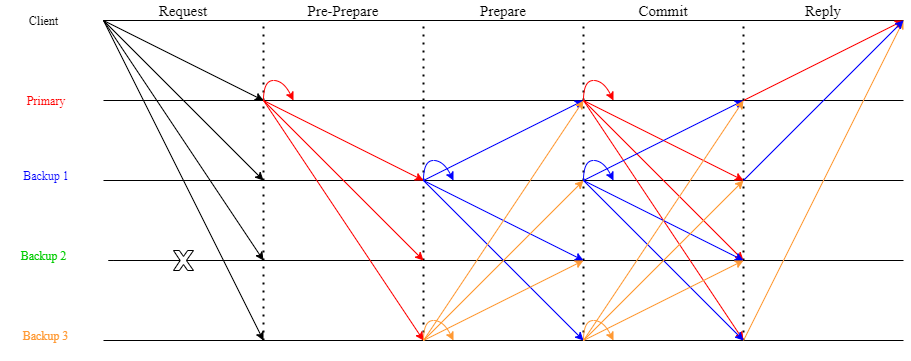
\includegraphics[width=\linewidth]{figures/PBFTWorkflow}
	\caption{Practical Byzantine Fault Tolerance Normal Workflow}
	\label{fig:pbftnormalworkflow}
\end{figure}

\section{Checkpointing}
\label{sec:checkpoint}
PBFT also incorporates checkpointing, which is a mechanism used for garbage collecting the logs. Checkpointing is required so that the replica does not use up all of its memory for logging messages~\cite[p.~261]{BOOK:BuildDepDistSyst}. Therefore, the replicas must agree upon a point in which the system is stable for all the replicas. Afterwards the replicas can delete any records in the logs prior to the consented state~\cites[p.~5]{PAPER:OGPBFT}[p.~410]{PAPER:PBFTRecovery}.

Checkpoints are essentially the state records of the system after progressing a specific interval of requests. The checkpoint has information regarding the last sequence number that was performed for the system. This sequence number is used on the garbage collector to put an upper bound on the records that are to be removed. For instance, if the stable sequence number was set to 50, then the garbage collector would remove a set of logged data up to 50. The checkpoint also has a digest of the system for that stable sequence number. This digest is used to confirm that the replicas have the same system state for the given sequence number~\cites[p.~5]{PAPER:OGPBFT}[p.~410]{PAPER:PBFTRecovery}.

In order for replicas to be able to validate checkpoints, they each must multicast a checkpoint message over the network containing the information mentioned above with its own replica id. Like the rest of the PBFT protocol messages a checkpoint is considered to be valid for a replica if it has stored $2f+1$ checkpoint messages with different replica id`s with the same stable sequence number and system digest~\cites[p.~261-262]{BOOK:BuildDepDistSyst}[p.~5]{PAPER:OGPBFT}[p.~410]{PAPER:PBFTRecovery}. Once a checkpoint has been validated successfully it is referred to as a stable checkpoint~\cites[p.~3]{PAPER:DPBFT}[p.~261]{BOOK:BuildDepDistSyst}. The replical usually stores checkpoint messages for different sequence numbers in memory and has only a single record for a stable checkpoint. Once a new stable checkpoint is determined, any checkpoint records with lower sequence numbers are removed from memory and if there exists a previous stable checkpoint in memory with a lower sequence number, then it is replaced by  the new one~\cite[p.~261-262]{BOOK:BuildDepDistSyst}.

In PBFT checkpointing is usually performed periodically after a constant number of requests have been processed. This interval length is constant and is referred to as a checkpoint period~\cites[p.~261]{BOOK:BuildDepDistSyst}[p.~410]{PAPER:PBFTRecovery}. As mentioned earlier in~\autoref{sec:detailedProtocol} PBFT normally only processes a sequence number if it is in the set of currently available sequence numbers. The length of the sequence number interval is usually designed to follow the format $[checkpointinterval+1-2*checkpointinterval]$. Which means the system attempts to calculate two checkpoints during a single sequence number interval. Once a stable checkpoint is obtained, the system extends the sequence number interval where the new interval starts at the last stable sequence for the current stable checkpoint~\cites[p.~5]{PAPER:OGPBFT}[p.~410]{PAPER:PBFTRecovery}. Unless a replica has exceeded the upper bound of the sequence number interval, the replical usually performs the checkpoint functionality concurrently to the protocol workflow.

\section{View-change}
\label{sec:view-change}
In the scenario in which the primary is the faulty replica, a view-change eventually occurs. The purpose of the view-change is to reassign the responsibility for a primary away from the current primary replica that is deemed to be faulty. Which is then given to another replica that is not faulty~\cites[p.262]{BOOK:BuildDepDistSyst}. As mentioned in \autoref{sec:systemModel}, the replica that is chosen as the next primary is based on the replica id and the next view number. Therefore, the view-change updates the view number for the system in order to change the primary replica of the system. There are some operations that need to be performed for a view-change to be deemed successful. The first operation is to update the view number to set another replica as the primary~\cites[p.~6]{PAPER:OGPBFT}[p.~411]{PAPER:PBFTRecovery}{WEB:SawtoothPBFT}. This step includes multicasting view-change messages between replicas to start the new view session. The other more demanding operation is that the primary needs to make sure that the system is stable and that replicas start the new view with the exact same system state. Therefore, all requests that have been performed after the last stable sequence number, need to be reprocessed between the replicas. This is done so that the system can guarantee that the replicas are not missing any of the previous operations performed to the system.~\cites[p.~458]{BOOK:MVstandver3}[p.~263-265]{BOOK:BuildDepDistSyst}.

There are several ways for a replica to deem its primary to be faulty, the most common way is to have a timeout functionality for the protocol execution. It is most common to start a timeout once a replica has received a request from the client. If the replica does not receive any pre-prepare messages for that request before the timeout expires, than the replica goes into view-change mode and no longer participates in any of the protocol operations~\cites{SLIDES:PBFT}[p.~5-6]{PAPER:OGPBFT}[p.~263]{BOOK:BuildDepDistSyst}.  

The view-change process starts by having the replica increment its view number. Then the replica creates, signesand multicasts a view-change message over the network. The replica  then waits for $2f+1$ view-change messages~\cites{SLIDES:PBFT}[p.~6]{PAPER:OGPBFT}[p.~411]{PAPER:PBFTRecovery}{WEB:SawtoothPBFT}. A timeout is also used here, if the replica does not receive enough view-change messages in time, then the process repeats with the next incremental view number. In some cases a replica can also be designed to go into view-change mode if a replica has already received two view-change messages from other replicas, as it now only requires its own view-change message for the system to agree that a view-change is necessary\cite{BOOK:BuildDepDistSyst}. Once the appropriate number of view-change messages are received, then the new primary is responsible for creating, signing and multicasting a new-view message to the other replicas~\cite[p.~264]{BOOK:BuildDepDistSyst}. Before the new-view message can be multicast to the other replicas, a new primary must go through its log and create new pre-prepare messages for all sequence numbers that have occurred after the last stable sequence number. If the new primary lacks a record in the log for any of the sequence numbers, the new pre-prepare message has its request digest be set to be \code{null}. This information is included in the new-view message, which is then sent to the other backup replicas. The backup replicas then validates and re-process each of the sequence numbers that have a valid pre-prepare message. This essentially means that the other replicas have to multicast a new prepare message and then participate in a commit phase together with the new primary for each of the pre-prepare messages in the new-view message~\cites[p.~6]{PAPER:OGPBFT}[p.~458]{BOOK:MVstandver3}[p.~265]{BOOK:BuildDepDistSyst}. A timeout is once again being used to handle the situation where the reprocessing takes too long. This process can also fail if the pre-prepares in the new-view message fails the validation process. If either the timeout occurs or the validation fails, then it is back to the start for the view-change process. Once all pre-prepares have been reprocessed, the view-change procedure is over, and the replica returns to normal protocol operations with the new chosen primary. Keep in mind that any new requests received during the view-change process are ignored by the system~\cite[p.~263]{BOOK:BuildDepDistSyst}. 

\autoref{fig:pbftviewchange} shows an example of a view-change process. The figure shows the timeline for each of the processes needed for the view-change to be successfully completed. Starting with the timeout occurring on the backup replicas when the primary is no longer working properly. Then the replicas each multicast a view-change message to the other replicas in the system, including the faulty primary. After the new primary has received a sufficient number of view-change messages, it creates pre-prepares messages that need to be reprocessed in the network. Afterwards the new primary multicast new-view messages to the other replicas to start the re-processing phase. Finally the system multicasts both prepare and commit messages to validate pre-prepare messages. Once all that is done the system moves on to normal workflow again with the first backup replica now serving as the primary for the system.

\begin{figure}[!h]
	\centering
	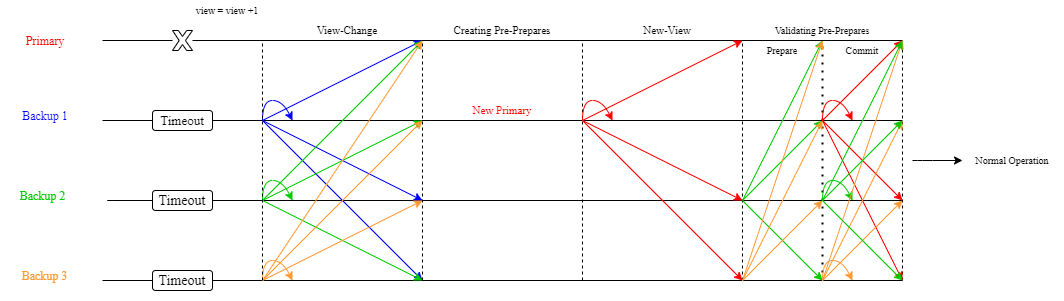
\includegraphics[width=1.1\textwidth]{figures/PBFTViewChange}
	\caption{Practical Byzantine Fault Tolerance View-Change}
	\label{fig:pbftviewchange}
\end{figure}

%In the scenario in which the primary is the fault replica, a view-change occurs. The purpose of the view-change is to reassign the primary responsibility away from a replica that is deemed to be faulty. As mentioned in \autoref{sec:systemModel}, the replica which is chosen as the primary is based on the replica id and the current view number. Therefore, the view-change updates the view number to update the primary replica. There are 3 main operations that need to be performed for a view-change to be deemed successful. The first is to update the view number to set another replica as the primary. The second is to validate this new leader on whether it is a suitable replacement. Finally, all operations that are performed after the last stable checkpoint needs to be reprocessed between the replicas. There are several ways for a replica to deem its primary to be faulty, the most common way is to have a timeout functionality for the protocol execution. The one that is most common is to start a timeout once a replica has received a request from the client. If the replica does not receive any pre-prepare messages for that request before the timeout expires, the replica will go into the view-change mode and will no longer participate in any of the protocol operations.  

%The view-change process starts by having the replica increment its view number. Then the replica will create, sign and multicast a view-change message. The replica will then wait for $2f+1$ view-change messages. A timeout is also used here, if the replica does not receive enough view-change messages in time, then the process repeats with the next incremented view number. In some cases a replica can also be designed to go into view-change mode if a replica has already received two view-change messages from other replicas, as it now only requires its own view-change message for the system to agree upon the view-change. Once the appropriate number of view-change messages are received, then the new primary will be responsible for creating, signing and multicasting a new-view message to the other replicas. Before the new-view message can be multicast to the other replicas, a new primary must go through its log and create new pre-prepares for all sequence number that has occurred after the last stable sequence number. If the new primary lacks a record in the log for any of the sequence numbers, the new pre-prepare message will have its request digest be set to null. This information is included in the new-view message, which is then used by the other replicas to validate and re-process each of the sequence numbers that has a valid pre-prepare. This essentially means that the other replicas have to multicast a new prepare message and then participate in a commit phase together with the new primary for of the pre-prepare messages in the new-view message. A timeout is once again being used in the case where the reprocessing fails or takes too long. This process can also fail if the pre-prepares in the new-view message fails the validation process. If this happens, then its back to start and in the view-change process. Once all pre-prepares have been reprocessed, the view-change procedure is over, and the replica will return to normal protocol operations using the chosen new primary. Any requests received during the view-change process will be ignored by the system. 

%TODO rewrite after implementing the basics of view change for app
%In the scenario where the primary is the faulty replica a view change occurs. A view change increments the view number for all participating replicas, which in turn chooses as a new primary replica for the network following the formula mention in \autoref{section:systemModel}. 
%Normally each replica starts a timeout operation whenever it receives a request from a client~\cite[p.~415]{PAPER:PBFTRecovery}. 
%If the replica does not receive a pre-prepare message before the timeout expires, then the replica deems the primary to be faulty and desires a view change. The replica will multicast a view-change message to the other replicas in the view, including the potentially faulty primary, and will ignore any %new incoming messages with the exception of view-change, new view and checkpoint messages~\cites[p.~5-6]{PAPER:OGPBFT}[p.~263]{BOOK:BuildDepDistSyst}. 
%A replica receiving a view change will reply with a view-change-ack.  The new primary chosen will collect view-change messages and view-change-ack messages to create a view-change certificate. Once the certificate is valid and has reached $2f+1$ unique messages a new-view message is multicasted to %every replica in the network, officially starting the new view~\cites[p.~412-414]{PAPER:PBFTRecovery}[p.~263-p.265]{BOOK:BuildDepDistSyst}[p.~458]{BOOK:MVstandver3}.
%%PBFT also incorporates checkpointing, which is a mechanism used for garbage collecting the saved logs. Without checkpoints, the replica would eventually use up all of its memory for logging protocol messages~\cite{BOOK:BuildDepDistSyst}. 
%%Checkpoints are essentially a proof where the replicas have agreed on a stable state for the system after a specified interval of requests has been processed~\cite[p.~5]{PAPER:OGPBFT}. For instance, if the checkpoint interval was set to 50, then the system would only allow sequence numbers 0 to 50 to %be performed in the first interval. Once the checkpoint interval is reached the log data is hashed and saved as a checkpoint message. The message is then multicasted over the network. Consensus is reached when a replica receives $2f+1$ checkpoint messages with different identifiers, but they all have same checkpoint hash value. The checkpoint is then saved on the replica and all the protocol messages with lower or equal sequence number to the checkpoint interval will be deleted from the log. As an example, if the checkpoint interval was 50, then certificates saved up for requests 0 to 50 are deleted. Then the interval is updated to be $[checkpointinterval+1-2*checkpointinterval]$, so for the last example the new interval would be between 51 to 100~\cites[p.~3]{PAPER:DPBFT}[p.~5]{PAPER:OGPBFT}[p.~409-410]{PAPER:PBFTRecovery}[p.~p.261-262]{BOOK:BuildDepDistSyst}.

\iffalse
\cite[p.~415]{PAPER:PBFTRecovery}
\cite[p.~5-6]{PAPER:OGPBFT}
\cite[p.~263]{BOOK:BuildDepDistSyst}
\cites[p.~3]{PAPER:DPBFT}
\cite[p.~458]{BOOK:MVstandver3}
\fi

%\cite{WEB:PBFTGeeks}
%\cite{WEB:ImpPBFTBlock} %not used
%\cite{WEB:UnderpBFT} %not used
%\cite{WEB:PBFTConSeries} %not used
%\cite{SLIDES:PBFT}
%\cite{VIDEO:YPBFT}
%\cite{BOOK:MVstandver3}
%\cite{BOOK:BuildDepDistSyst}
%\cite{PAPER:OGPBFT}
%\cite{PAPER:DPBFT}
%\cite{PAPER:PBFTRecovery}
%\lstset{style=sharpc}
%\begin{lstlisting}
%Your c# code here
%class Request
%{
%	private m string;
%} 
%\end{lstlisting}	
	
	\chapter{Related Work}
%1-2 papesa
%If you cannot demonstrate that you know, and understand, what others have done, you only demonstrate that you're clueless. 
%For an undergraduate thesis this, together with a thorough understanding of the problem, should be the result of the first session's work. 
%It is an unfortunate fact that many students do very little work during the first session of their thesis. 
%It usually shows here (and is usually reflected in their mark). 
%Don't think you can fool your thesis supervisor/assessor. And don't even dream about fooling the referee of a paper. 
%If you haven't done your homework here, it's probably not worth going any further.
%In this part you demonstrate that you are aware of what's going on in the field, and how it relates to your particular problem.
%If there is lots of related work, discuss related work early to differentiate your own work
%-Compare/contrast with your own work - don't just enumerate
%-Don't be dismissive
%-Refer to references by author or project names
\label{chapter:RW}

The University of Stavanger has previously supported the development of Cleipnir. As a result has published papers and thesis in regards to its usage in consensus algorithm implementation. In particular two contributions have been used as building blocks for this project. We now discuss these two works in detail and explain how they contributed to our work.  

\section{Cleipnir - Framework Support for Fault-tolerant Distributed Systems}
This paper is the original paper describing the Cleipnir framework and is written by its creator Thomas Stidsborg Sylvest and co-written with two professors at the University of Stavanger Leander Jehl and Hein Meling. The paper describes, in detail, the internal functionality and tools available in the Cleipnir framework. This includes their use case, detailed explanation of how they work and practical demonstration for how to use them. The demonstrations are presented using an existing implementation of the Paxos consensus algorithm. The paper also presents a Raft implementation using the Cleipnir framework. This includes overall architecture of the implementation, detailed examples of usuage of Cleipnirs tools, and evaluation of experiments performed on the Raft implementation to measure its performance. The results of the experiments are compared directly to the Paxos implementation, both in terms of latency and code structure. Our thesis is a direct continuation of this paper with practically the same goals. The main difference between our thesis and this paper being the chosen consensus algorithm that are to be implemented using Cleipnir. Our contribution is to provide additional experiences on how well Cleipnir can be utilized in implement complex consensus algorithms. This also implies discovering potential difficult problems that the current Cleipnir framework is currently not able to handle. Specifically whether or not Cleipnir can handle all of the complex problems that can take place, while still upholding the program paradigm in a easy to read code structure~\cite{PAPER:PaxosCleipnir}.

\section{Implementing a Distributed Key-Value Store Using Corums}
In 2010, Eivind Bakkevig wrote a master thesis where his goal was to implement a distributed system which made decisions based on the Paxos consensus algorithm. The consensus algorithm was implemented using the Corums .Net framework. 

The Corums framework is the predecessor to Cleipnir and includes the same programming model that Cleipnir offers. These models would be the closely related to the ones described in \autoref{chapter:Cleipnir}, namely Built-in Persistency, Reactive programming and Single-Threaded scheduler. 
The main difference between Corums and Cleipnir is that Corums focus more on simplifying an abstraction for handling communication using incoming/outgoing communication bus. Cleipnir has more focus on getting the persistent programming paradigm into a consensus algorithm in a easy to use, and customizable way as possible. As an example, a major difference between Cleipnir and Corums lies in Corums support in reliable message delivery between distributed systems. Corums uses a simple Bus abstraction to easily handle incoming/outgoing messages between the nodes in the system. Cleipnir does not support this functionality~\cites[p.~6-7]{PAPER:PaxosCleipnir}{DOC:Cleipnir}.

Corums is very similar to Gorums~\cites[p.~2]{WEB:Gorums}[p.~22]{PAPER:EivindPaper} which is intended based on how close the names are, the main difference being the supporting language. 
Bakkevig succeeded in creating a distributed dictionary storage using the Corums framework. Additionally he built the client side programming using the existing ASP.NET Core Web API~\cite{WEB:ASPNetCoreAPI}. 

According to Bakkevig, he had no prior experience with the C\# before this thesis. Bakkevig did however had previous experience with the Paxos consensus algorithm. This made most of his work during the thesis about learning C\# and the Corums framework rather than having to extensively research Paxos. In terms of background this thesis has the exact opposite background. We have some background knowledge regarding the C\# language but had little to no knowledge regarding the PBFT algorithm. Therefore, a lot of work needs to be put into fully understanding the PBFT consensus algorithm, rather than focus fully on the Cleipnir framework. It is important to note that our work do not have any background experience with the Cleipnir framework just like Bakkevig had no prior experience with the Corums framework~\cite[p.~8]{PAPER:EivindPaper}.
	
	
	\chapter{Design}
\label{chapter:Design}
%Overarching design in a top-down view: 
%-server/client design overall architecture, system model
%-describe file system, 
%-how protocol is peformed by the server
%-describe current functionality of the implementation. Handles protocol run, view-changes and checkpointing

%old version:-overall usage over different parameters, overaching stuff thats not the actual implementation of the algorithm, but the network layer to server to algorithm, how to run the algorithm/checkpointing/view changes.
%first draft!!!
This chapter presents an overall summary of our \ac{pbft} application implementation. This includes a description of the system architecture used for the \ac{pbft} network. Additionally, to better understand the workflow of the application, a summary of our code structure is given. Finally, a description is provided for the current application design. Primarily specifying which parts of the program take advantage of the Cleipnir framework and how the server side interacts with the protocol workflow.
%Remember to check previous sections for how I should mark names in the text!
\section{Network Architecture}
\begin{figure}
	\centering
	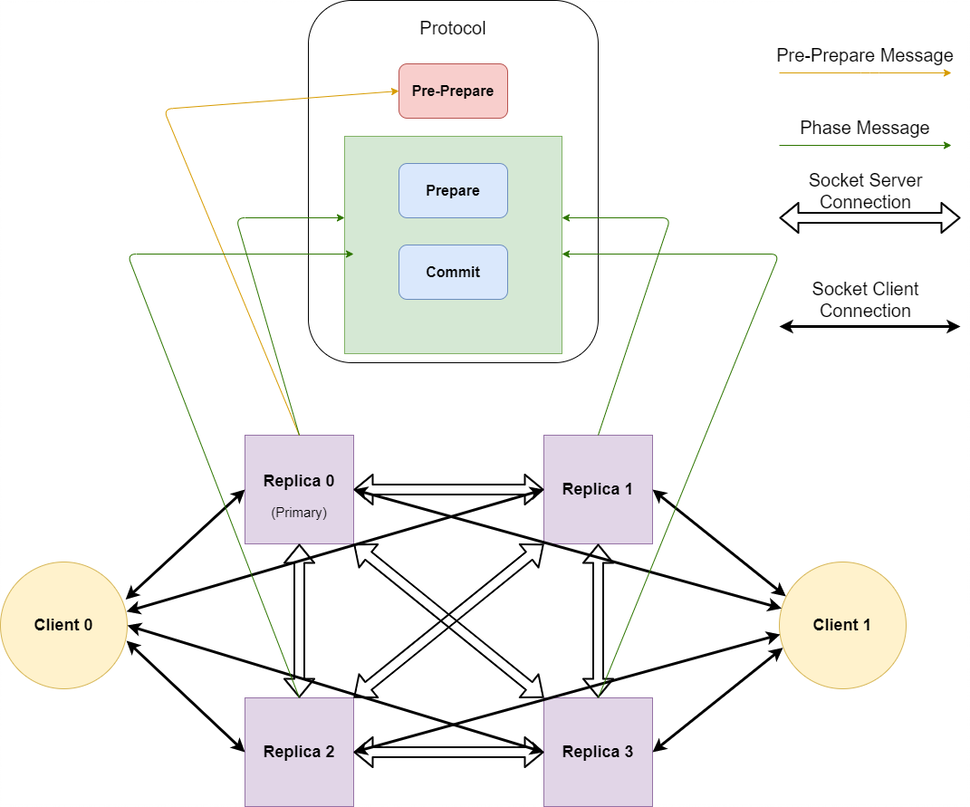
\includegraphics[width=\linewidth]{figures/meshnetwork}
	\caption{Overall architecture of the \ac{pbft} implementation networking}
	\label{fig:meshnetwork}
\end{figure}
%NEED TO REDESIGN SO THAT NETWORK IS MENTION IN ONE PART AND OTHER STUFF IN ANOTHER SUBTITLE
The \autoref{fig:meshnetwork} shows the system architecture used for \ac{pbft} implementation. Generally our network architecture follows the same structure as the system model introduced in \autoref{sec:systemModel}. The system consists of four server implementations called \emph{replicas}, where the replica with the lowest identifier value is chosen as the primary. These four replicas are communicating over a mesh network using socket connections. This means each replica shares a unique network socket with each other replica in the \ac{pbft} network. To avoid creating multiple socket connections between two replicas, the replica with the highest identifier is the one tasked with being the initiator when creating the socket connection. Because of this the primary replica is not required to be an active party when establishing any connections to its fellow replicas. The primary instead establishes all its socket connections by listening for any connection attempts on its local network address. The opposite scenario occurs for the replica with the highest identifier value. Although the replica still listens for connections on its local network address in the case where a higher replica does exist in the network, it is also responsible for initiating the socket connections with all the other replicas in the network that have lower identifier values to its own.

When the replicas have established connections, the replicas can still not fully communicate with each other until they have exchanged public keys. This is required so that messages between replicas can be verified using a digital signature. Public keys are exchanged in \emph{session messages}, which are messages that are automatically sent between replicas once a socket connection has been established. If the public keys are for some reason not exchanged, then the replica discards any message received from that host. If the message received from the unknown host happens to be a \emph{request} or a protocol related message, the replica also terminates the connection. This also applies for clients. This current public key model is unfortunately not very secure. This is due to public keys being ephemeral, therefore it needs to be updated and replaced in the case the replica’s execution is interrupted or stopped. Currently in this implementation, the private and public key pair for a replica are created randomly at system start-up. Currently there is no way for the replicas to authenticate another replica after it has rebooted. A replica must therefore replace the key value pair representing a replica's public key in its register if it receives a new session message with the same replica identifier value. This in turn means the system is susceptible to impersonation and spoofing attacks~\cite{WEB:spoofingAttack}. Because the main goal of this thesis focuses more on the aspects behind implementing a simple \ac{pbft} workflow, the current cryptographic system was deemed sufficient for simulating a network using digital signatures. However, it is important to be aware of this major security flaw of the system so that it can be potentially fixed in the future. Not to mention avoid similar problems in the future.


\section{Overview of Workflow}
The system performs the \ac{pbft} protocol by exchanging protocol messages over the mesh network until at least three of the servers have finished all three protocol phases. In this implementation protocol messages. The \ac{pbft} protocol is triggered when the server receives a request from one of the connected client nodes. The primary is responsible for officially starting an instance of the \ac{pbft} protocol by multicasting a protocol message of type pre-prepare. There are two important goals for the pre-prepare phase. The first is to make sure that the replicas have an agreement upon the ordering of the request. In other words, the replicas will perform the requests in the same order as the primary, which in turn means the request should have the same sequence numbers throughout the network. The second important goal is to determine whether or not the primary is fit to be leader. As mentioned in section \autoref{sec:view-change}, a view-change occurs when a leader no longer is eligible. In our application the view-changes are triggered by timeout which are set once a replica receives a client's request. If the primary takes too long in the pre-prepare phase, then the timeout will exceed and the other replicas will perform a view-change in order to change the primary replica. Although it would be useful to have timeouts in the commit phase in the instance where the majority of servers are unable to properly finish the commit phase, it is currently not supported in our implementation due to how timeouts are handled inside the protocol workflow(should probably be moved elsewhere). The rest of the replicas will be the responsible party during the prepare phase by sending protocol messages of type prepare, while every replica will participate in the commit phase using commit type protocol messages. The last step of current \ac{pbft} implementation is to create a reply message and send it back to the client responsible for the request. The details in regards to the \ac{pbft} workflow implementation will be discussed in \autoref{chapter:Imp}.

\section{Code structure}
In the figure we \autoref{fig:filestruct} can see a short summary of the code structure for our \ac{pbft} replica. The summary shows folders containing our implementation for necessary items for the \ac{pbft}. The summary also highlights some of the more important files, meaning files that contain the most relevant code segments for the application.

%REWRITE SO THAT THE FOCUS IS ON THE Code structure how protocol functionality is %divided into different class objects and divided etc. Then talk about the server.cs <--> %workflow relationship, started by App.cs

\subsection{Protocol Objects}
To start off, the \ac{pbft} algorithm uses a lot of different types of message for the replicas to collaborate. For simplicity we stored all of the classes revolving messages within the \emph{Message} folder. Since the protocol messages share traits and functionality, we introduced two interfaces to reduce redundancy. The first interface regards the serialization process for transforming the messages into byte streams so that they can be exchanged over the \ac{tcp} network~\cite{WEB:tcp}. The other interface is for the digital signature process. Session messages are not signed, therefore they do not inherit this interface. In addition, to reduce complexity we set the normal workflow protocol messages such as pre-prepare, prepare and commit messages, to use a single class object known as \code{Phase Messages}. View-change and checkpoint messages are instead represented with their own unique class object.

To store the proof of an \ac{pbft} iteration, we implemented class objects known as \emph{certificates} that are found in the \emph{Certificates} folder. The implemented certificate objects essentially have the same functionality as the different certificates described in \autoref{chapter:PBFT} for the \ac{pbft} algorithm. Certificates act as records showing the status of the state of protocol iteration, where a single iteration requires 2 valid certificates in order to finish. Just like the protocol messages, we implement both protocol certificate types by an object class known as \code{Protocol certificate} where the protocol types are determined by a single variable. Checkpoints and view-changes once again have their own class object for their certificate proof. There are also interfaces used to avoid redundant code for the certificate objects.

\subsection{Other functionalities}
The static functionalities that are not tied to any object classes are placed in the \emph{Helper} folder. This includes functionality for serializing and deserializing messages objects with \ac{json}~\cite{WEB:NewJSON}, cryptographic functions related to creating and validating digital signatures and files containing all the enum types used for this implementation. An enum is essentially a predefined dotnet class that has only constant values which are defined upon initialization and is really useful for classifying other objects~\cite{WEB:Enum}. In our \ac{pbft} implementation we have for instance used enums to categorize the protocol phase a phase message belongs to. This allows the program to easily distinguish between pre-prepare, prepare and commit phase messages even when they all use the same object type.

The \emph{JSONFiles} folder contains the \ac{json} files which have information about the network addresses for each of the replicas in the system designated to their receptive identifier values. There exist two \ac{json} files in this folder. The first file is used when running the implementation over multiple systems or over docker containers. The second file uses localhost addresses with different port numbers that are meant to be used when testing the system on a local device.

The \ac{pbft} replica implementation uses Cleipnir to persist important parts of the code in order for servers to easily be able to reconnect to the system. As discussed in \autoref{chapter:Cleipnir}, Cleipnir has several different engine types which can be used to serialize and store the applications data. In our \ac{pbft} replica implementation, we have decided to use the \emph{Simple File Storage} engine. The \emph{Storage} folder will contain the .txt files in which Cleipnir stores its data in. Since there are several instances of replicas in the \ac{pbft} network, the name of the .txt file used to store the application data will follow the structure "PBFTStorage" with the replicas identifier value at the end of the name.

The \emph{Replica} folder contains code which is directly related to the server or code which are directly related to the protocol. The \emph{Replica} folder has two sub folders in order to easier distinguish code based on their functionality. All the networking code that is not directly connected to the server side network handling is placed inside the subfolder \emph{Network}. This includes the code for creating sockets and functions for properly handling the data received from the socket by the TCP network protocol.
The \emph{Protocol} sub folder contains code which is directly related to the protocol execution. This includes code related to the execution of the main workflow of the \ac{pbft} algorithm. In addition, code for handling the reactive execution for view-change and checkpointing are also placed here.
The other files in the \emph{Replica} folder contains code that helps the replica run properly, including code which is used to help communication between server side and protocol workflow run inside Cleipnir.

\subsection{JSON Serialization Problem}
As mentioned in \autoref{section:PersistentProgramming} Cleipnir requires a designated serializer and deserializer function in order to persist an object. In addition, Cleipnir cannot persist traditional data structures directly. Instead Cleipnir intends for the developer to substitute traditional data structures with Cleipnir respective inbuilt data structures. This means that whenever Cleipnir persists objects that have a reference to a data structure, then the persisted object must also substitute the data structure for correct inbuilt Cleipnir data structure. For our case this is present for all of our \code{Certificate} objects as they all require a list of proofs. Therefore in order to persist the proof list, we need to replace a traditional \code{List} class object with an inbuilt \code{CList} class object. However, Cleipnir inbuilt data structures cannot be serialized or deserialized properly using \ac{json} formatting. As we were not completely aware of this issue when we began designing our application, we unfortunately made an oversight for our network layer. The application currently uses \ac{json}~\cite{WEB:NewJSON} to serialize and deserialize messages when sent over the \ac{pbft} network. Since \ac{json} formatting does not support inbuilt Cleipnir data structures, which in retrospect was not all that surprising, attempting to deserialize any protocol message that includes an inbuilt Cleipnir data structure, causes the application to crash. Currently we solve this issue by converting between traditional data structures and inbuilt Cleipnir data structures whenever a message with said data structure is to be serialized with \ac{json}. The conversion itself is rather primitive. A copy of the data storage in the traditional data structure format is created, then the content is copied from the source data storage to the newly created data storage. The process is then reversed on the receiver end after the message has been properly deserialized. To further simplify the conversion between the data structure types, we added temporary \code{\ac{json}} class objects that acts as substitutes for the persisted objects that have issues with \ac{json} when they are to be sent over the \ac{pbft} network. Transforming between a persisted object to their respective temporary \ac{json} object is as simple as making a function call with the opposite transformation also available. These \ac{json} objects are all placed in the subfolder \code{JsonObjects} in the \code{Helper} folder. All implemented \ac{json} class objects follow the naming convention $JSON + Objectname$. Having now learned about this issue it properly would have been more beneficial if the serialization and deserialization for the networking used the same formatting in which Cleipnir supports, as to avoid this issue in the future projects.

%In order for this to be done the persistable objects needed to be assigned a serializer function and deserializer function for Cleipnir to use. This also includes using Cleipnir inbuilt data structures when the persisted objects needed to also persist data stored in data structures. This is especially present in certificates since they need to persist their list of proofs, meaning the proof list uses the inbuilt Cleipnir \code{CList} to substitute normal List class objects. Unfortunately we made an oversight when we designed the application. The application currently uses \ac{json}~\cite{WEB:NewJSON} to serialize and deserialize messages when sent over the \ac{pbft} network. \ac{json} formatting does not support inbuilt Cleipnir data structures, which is not surprising yet was not directly discovered until very late into the \ac{pbft} implementation. Currently this issue is solved by converting between traditional data structures and inbuilt Cleipnir data structures whenever a message with said data structure is to be serialized by \ac{json}. The conversion itself is rather primitive. A copy of the data storage in the traditional data structure format is created, then the content is copied from the source data storage to the newly created data storage. The process is then reversed on the receiver end after the message has been properly deserialized. Although in retrospect, it might have been more beneficial if the serialization and deserialization for the networking used the same format in which Cleipnir supports, as to avoid this issue in the future

\subsection{Notable Files}
The \emph{App.cs} file contains the code which starts all the processes needed in the \ac{pbft} replica. This includes code for starting Cleipnir, creating a server instance and starting the protocol handlers. This file also includes the main application state, which in this implementation is simply a list of operations theoretically performed by the system.

The \emph{Server.cs} file is by far the largest. This is due to the server this implementation  acts as the bridge linking the network layer, responsible for sending and receiving messages properly, to the active protocol workflow which requires the result of said messages. In general the server is also responsible for the other server side operations.

The \emph{Workflow.cs} file is where the code for normal protocol workflow and view-change workflow occurs. The \autoref{chapter:Imp} introduces in detail how the workflows are implemented.
%\newpage
\begin{wrapfigure}{r}{0.45\linewidth}
\centering
%\vspace{15pt}
%\rule{0.9\linewidth}{0.75\linewidth}
% ,scale=0.8, every node/.style={scale=0.8}
\tikzstyle{every node}=[draw=black,thick,anchor=west]
    \begin{tikzpicture}[%
      grow via three points={one child at (0.5,-0.7) and
      two children at (0.5,-0.7) and (0.5,-1.4)},
      edge from parent path={(\tikzparentnode.south) |- (\tikzchildnode.west)}]
      \node {PBFT}
        child { node {App.cs}}
        child { node {Certificates}
        	child {node {...}}
        	}	
        child [missing] {}
        child { node {Messages}
        	child {node {...}}
        	}
        child [missing] {}
        child { node {Helper}
        	child {node {...}}
        	}
        child [missing] {}
        child { node {JSONFiles}
        	child {node {serverInfo.json}}
        	child {node {testServerInfo.json}}
        	}
        child [missing] {}
        child [missing] {}
        child { node {Storage}
        	child {node {...}}
        }
        child [missing] {}
        child { node {Replica}
          child { node {Server.cs}}
          child { node {Network}
          	child {node {...}}
        	}
        }
        child [missing] {
          child { node {Protocol}
          child { node {Workflow.cs}}
          child { node {...}}
        	}
        };
\end{tikzpicture}
    \caption{Summary of the file architecture for the PBFT implementation}
    \label{fig:filestruct}
    \vspace{40pt}
\end{wrapfigure}

\begin{figure}[H]
	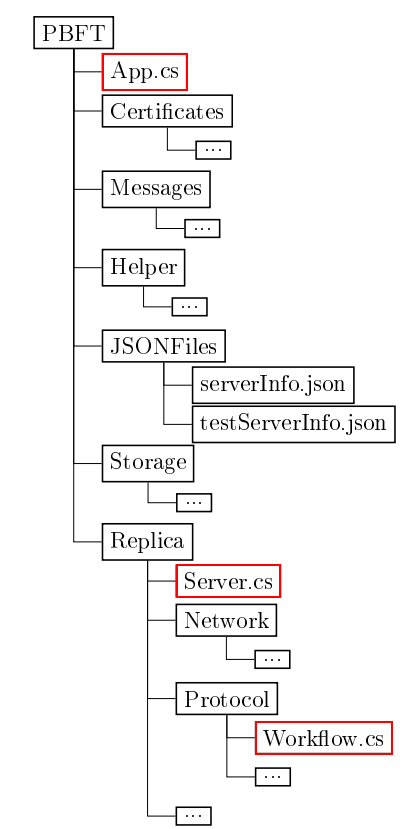
\includegraphics[width=0.45\linewidth]{figures/filestructtest}
	\caption{Summary of the file architecture for the \ac{pbft} implementation}
    \label{fig:filestruct}
\end{figure}

\newpage

\section{Persistent vs Ephemeral}
%This will be a very large part, just need to figure out how to structure it.
%Before we can introduce the main PBFT implementation workflow, it is first important to introduce the relationship between the server side and the protocol workflow.
%\label{sec:persvsephe}
%An important detail when using the Cleipnir framework is to have a general idea for which parts of the system are desired to be persistent. As mentioned in \autoref{section:PersistentProgramming}, Cleipnir allows for hybrid persistent programming allowing the developer the freedom to choose which parts of the application to persist while keeping the rest of the data ephemeral. In our case it was important to figure out which data needed to be persisted in order for the \ac{pbft} algorithm to be easily reinstated should the system shutdown. In addition, when taking advantage of hybrid persistent programming it is important to avoid storing a lot of unnecessary data as it generally slows down the synchronization period. Another reason as to why making a distinct divide between persistent and ephemeral parts of the code is important is due to the difficulties encountered when using \code{CTask} together with traditional asynchronous operations as mentioned in \autoref{section:PersistentProgramming}. In our case, because our goal is to evaluate both async/await and Cleipnir for implementation of consensus algorithms, it is important to not interchange these tools as it would in most cases lead to race conditions.

%\autoref{fig:PersistencyEphemeral} we show parts of our \ac{pbft} implementation that are divided into persistent parts and ephemeral parts. In addition the figure shows an illustration as to how ephemeral parts and the persistent parts collaborate using arrows to dictate the program flow. In general for our application, static functions and objects unrelated to the \ac{pbft} workflow are treated as ephemeral. Meanwhile objects related to the \ac{pbft} implementations, \code{Source} objects and functions that handle workflow related to the \ac{pbft} protocol are persisted. The server is an exception as some parts are persistent while others parts are not. As an example, the protocol logger is stored in the server and is persisted, on the other hand any code related to networking in the server is not persisted. In a sense we can view some of the operations occurring in the server as being treated as a bridge between the persistent parts as well as the ephemeral parts. By this we mean that the server is responsible for handling any messages received from the ephemeral socket connections and delivering them to the appropriate protocol workflow that is persistent. 

%These messages are then emitted to their respective reactive operators which are run in the persistent part and are waiting for changes to occur. There are a few exceptions to this rule, case in point if the message is needed for server-side rather than any \ac{pbft} protocol workflows, the message is instead used directly by the server. A primary example of this being session messages. However, in order for the server's non-persistent network handler to perform operations which affect the persistent part run by Cleipnir, the operation must be scheduled by Cleipnir's execution engine. There are two reasons for this syntax. 

%Firstly, code run by Cleipnir is not supposed to be affected by code outside of Cleipnir. Similarly to the case where using asynchronous operations within \code{CTask}, attempting to emit a message or perform an operation which changes the state of a persisted object, will most of the time cause the same scenario we discussed earlier in \autoref{chapter:Cleipnir}. New threads are created and Cleipnir attempts to perform the operation concurrently, however this scenario is not thread safe and sooner or later causes issues for the state of the system negatively. 
%\ac{fcfs}
%Secondly, running operations though the Cleipnir's execution engine attempts to enforce the operations to be run in a \ac{fcfs} approach as mentioned in \autoref{section:CleipnirOv}. This will in turn make it a lot easier to keep track of the operations as it gives the illusion of a synchronous system. The only situation we experienced where the Cleipnir execution engine didn't follow the \ac{fcfs} scheduling algorithm was when the next operation was stuck, in which the second operation in the queue line was executed instead and so forth. \autoref{code:schedulerEmit} shows an example of where the server uses the Cleipnir engine reference to schedule a phase message to be emitted to the \emph{ProtocolSubject} \code{Source} object. To summarize the primary relationship between the server, the network layer and the persistent workflow implementations is simply that the server will emit any messages it receives from the network layer and then emit these messages to the persistent workflows. As it is required for the \ac{pbft} protocol and view-change protocol to multicast messages during their process, these implementations have a direct reference to the server. In order to accomplish this, both persistent workflow shares a common persistent object known as \code{ProtocolExecution}. This means the protocol algorithms can easily send any messages it needs to the server through the server referance in the \code{ProtocolExecution}. REWRITE NOWWWWW

%This design is unfortunately not perfect. Because the server is required to schedule the operations in order for protocol execution to move on with its execution. We have encountered some situations where the scheduled process never finishes its execution. This wouldn’t be considered a big issue most of the time as the application is run asynchronously, however there are some instances where this situation can become a big problem.. Usually when scheduling an operation which requires emitting an object to a \code{Source} object that currently does not have any receivers, the operation obviously never finishes. When the server attempts to schedule an additional operation afterwards, the operation is never scheduled, which in turn leads to the application being deadlocked. This situation seems to be similar to sending messages to a channel without any receivers in Golang~\cite{WEB:golangChannels}, in spite of that this is an issue which rarely occurs, but when it does it is detrimental to the system. Therefore, to counteract this issue, strict conditions are placed in the server to avoid sending messages to reactive subjects in the situations where there are no listeners.

\label{sec:persvsephe}
An important detail when using the Cleipnir framework is to have a general idea for which parts of the system are desired to be persistent. As mentioned in \autoref{section:PersistentProgramming}, Cleipnir allows for hybrid persistent programming allowing the developer the freedom to choose which parts of the application to persist while keeping the rest of the data ephemeral. In our case it was important to figure out which data is needed to be persisted in order for the \ac{pbft} algorithm to be easily reinstated should the system shutdown. In addition, when taking advantage of hybrid persistent programming it is important to avoid storing a lot of unnecessary data as it generally slows down the synchronization period. Another reason as to why making a distinct divide between persistent and ephemeral parts of the code is important is due to the difficulties encountered when using \code{CTask} together with traditional asynchronous operations as mentioned in \autoref{section:PersistentProgramming}. In our case, because our goal is to evaluate both async/await and Cleipnir for implementation of consensus algorithms, it is important to not interchange these tools as it would in most cases lead to race conditions.

\autoref{fig:PersistencyEphemeral} we show parts of our \ac{pbft} implementation that are divided into persistent parts and ephemeral parts. In addition the figure shows an illustration as to how ephemeral parts and the persistent parts collaborate using arrows to dictate the program flow. In general for our application, static functions and objects unrelated to the \ac{pbft} workflow are treated as ephemeral. Meanwhile objects related to the \ac{pbft} implementations, \code{Source} objects and functions that handle workflow related to the \ac{pbft} protocol are persisted. The server is an exception as some parts are persistent while others parts are not. As an example, the protocol logger is stored in the server and is persisted, on the other hand any code related to networking in the server is not persisted. In a sense we can view some of the operations occurring in the server as being treated as a bridge between the persistent parts as well as the ephemeral parts. By this we mean that the server is responsible for handling any messages received from the ephemeral socket connections and delivering them to the appropriate protocol workflow that is persistent. 

These messages are then emitted to their respective reactive operators which are run in the persistent part and are waiting for changes to occur. There are a few exceptions to this rule, case in point if the message is needed for server-side rather than any \ac{pbft} protocol workflows, the message is instead used directly by the server. A primary example of this being session messages. However, in order for the server's non-persistent network handler to perform operations which affect the persistent part run by Cleipnir, the operation must be scheduled by Cleipnir's execution engine. There are two reasons for this syntax. 

Firstly, code run by Cleipnir is not supposed to be affected by code outside of Cleipnir. However, since the protocol workflow relies on messages from the non-persistent network layer this cannot be avoided in our application. Therefore a way for the persistent and non-persistent areas to work together must be coordinated. To start, attempting to emit a message to a \code{Source} object or perform an operation which changes the state of a persisted object outside of a \code{CTask} function, can cause the same scenario we discussed earlier in \autoref{chapter:Cleipnir}. That is, new threads are created and Cleipnir attempts to perform the operation concurrently, however this scenario is not always thread safe and sooner or later causes issues for the state of the system negatively. 

It is intended to avoid this problem by using the Cleipnir execution engine directly to schedule the desired operation to be run with Cleipnir support. The Cleipnir execution engine runs its scheduled operations using a \ac{fcfs} approach as mentioned in \autoref{section:CleipnirOv}. Scheduling operations desired for the protocol using the execution engine makes it easier to keep track of operations as they must likely run in a synchronous order with the other operations happening in the protocol workflow. This however this not mean the system is synchronous as Cleipnir only gives an illusion of a synchronous system. The execution engine can change the order of execution while another scheduled operation is idle or stuck.In which case the next scheduled operation is run next. \autoref{code:schedulerEmit} shows an example of how to schedule an operation to the Cleipnir execution engine. In this example where the server schedules a phase message to be emitted to the \code{ProtocolSource} \code{Source} object.

To summarize the relationship between the server, network layer and the persistent protocol workflows is that the server is responsible for emitting any relevant messages received from the network layer to the protocol workflow. In addition, the server is also responsible for preparing and sending any protocol messages it gets from the protocol workflow to the network layer so that the protocol messages are correctly sent to the other replicas in the network. In order for the protocol workflows as an object reference to the server, meaning the protocol workflow calls the appropriate send function in the server object whenever a protocol needs for a protocol message to be sent over the network. Since both the normal protocol workflow and view-change workflow requires multicasting protocol messages to move on in their respective workflows, it is necessary for the workflows to have a direct reference to the server. All protocol workflow that requires the server referanse are all apart of the class known as \code{Workflow} 

This design is unfortunately not perfect. The server is required to schedule the operations in order for the protocol execution to move on with its execution. We have encountered some situations where the scheduled operations to the Cleipnir execution engine never finishes its execution. This wouldn’t be considered a big issue most of the time as the application is run asynchronously, however there are some instances where this situation can become a big problem. Usually when scheduling an operation that requires emitting an item to a \code{Source} object that currently does not have any receivers, the operation obviously never finishes. When the server attempts to schedule an additional operation afterwards, the operation is never scheduled, which in turn leads to the application being deadlocked. This situation seems to be similar to sending messages to a channel without any receivers in Golang\cite{WEB:golangChannels}, in spite of that this is an issue which rarely occurs, but when it does it is detrimental to the system. Therefore, to counteract this issue, strict conditions are placed in the server to avoid sending messages to reactive subjects in the situations where there are no listeners.

\begin{figure}[H]
	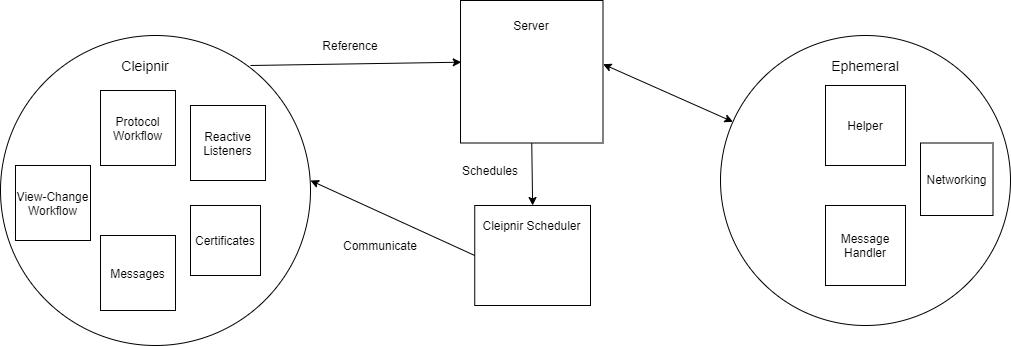
\includegraphics[width=\linewidth]{figures/CleipnirStructure}
	\caption{Application divided into persistent parts and ephermeral parts and how they interact}
	\label{fig:PersistencyEphemeral}
\end{figure}

\begin{figure}[h]
	\centering
	%\lstset{style=sharpc}
	\begin{lstlisting}[label = code:schedulerEmit, caption= Example of server and protocol interaction using Cleipnir scheduler, captionpos=b, basicstyle=\scriptsize]
public void EmitPhaseMessageLocally(PhaseMessage mes)
{
    Console.WriteLine("Emitting Phase Locally!");
    if (ProtocolActive)
    {
        _scheduler.Schedule(() =>
        {
            Subjects.ProtocolSubject.Emit(mes);
        });   
    }
}
	\end{lstlisting}
\end{figure}
	
	
	\chapter{Implementation}

%Implementation 
%describe code, but not to detailed
%motivation for using this design
%good parts/bad parts
\label{chapter:Imp}
%Implementation talks about the actual algorithm implementation that is run in protocol execution, includes process of checkpoints and view-changes. Should have figures to simplify explanation. Go over briefly the different phases, show some pseudocode. keeps to take note of, maybe include a model to show the persistency layers present. The importance of using the Cleipnir scheduler and CTask, where you have used them etc.

%outline aka what needs to be talked about, note not in any particular order
%detailed explanation of how the general workflow for the PBFT algorithm is performed, with code snippets.
%the simplicity of some of the necessary tools needed in PBFT is handled. Object oriented programming for Messages, Certificates. Static function for workflow, including Listeners, and handlers
%detailed explanation for how the checkpointing are handled
%detailed explanation for how the view-changes are handled
%Describe how you though of persistency during implementation(not much since its not general focus, and ofcourse doesn't work fully)
%small description on how clients are working, how they use the same reactive operators to count number of replies received.
%Add comment on how well they work, don't work do to design, this is an evaluation afterall.

In this chapter we introduce our \ac{pbft} implementation. We will introduce the implementation for the request handler, normal protocol workflow, view-changes, and finally checkpointing. We will also discuss how the Cleipnir framework is used to create the working \ac{pbft} implementation, as well as discuss some benefits and limitations within the current implementation design.

\section{Motivation}
%Motivation is supposed to be short and summarize these points:
%why did we implement our application the way we did, what was the main focus
%-Usage/testing the usage of the tools
%	-Simplicity --> Protocol description as close to possible
%-Some thought went into persistency due to Cleipnir, CTask for protocol workflow, persisted objects gets assigned Sync/Desync funcs
%-async used for networking
With the goal of the thesis in mind, the \ac{pbft} protocol workflows were designed to be as close defined to the protocol description as possible. To accomplish this, we believed the best approach would be to design protocol-related workflow as synchronous as possible. Several factors persuaded us to focus on keeping the protocol operations mostly synchronous. The first reason was that it is generally easier for developers to keep track of the program progress, making it easier to debug. Modern async/await can generally achieve a similar program workflow. Still, unless you are worried about blocking the main thread, there are no added benefits in terms of complexity or efficiency in using asynchronous programming. The second reason is in regards to Cleipnir. We previously discussed in \autoref{sec:persvsephe} and \autoref{section:PersistentProgramming} using normal asynchronous operations inside a function that uses Cleipnir is not a good idea. Because we wanted to take advantage of reactive programming to handle protocol-related messages in our protocol workflow, we needed to use Cleipnir reactive framework. Since persistency is a core part of the Cleipnir framework, we decided it was best to keep persistency in mind while designing our application. Therefore we decided to keep our protocol implementations inside \code{CTask} functions. Because of this, the only form of asynchronous operations that are performed inside any of the protocol workflows are restricted to other \code{CTask} asynchronous operations. The \code{await} operator still works the same as it does for traditional asynchronous operations. This allows us to take advantage of the \code{await} to set waiting points for \code{CTask} operations as well as ongoing reactive streams; Thereby giving the protocol the abstraction of a synchronous process, even though, in reality, it is an asynchronous process. 
To enable Cleipnir to persist in our protocol workflow, we also had to make sure that objects we wanted to persist in the protocol were persistable. To accomplish this we initialized both a serializer and deserializer functions for Cleipnir that follows the format specified in \autoref{section:PersistentProgramming} to use for each of our defined protocol objects.  
Finally, we have done our best to avoid creating circular dependencies. Circular dependencies would essentially cause the serialization process to fail, as it would lead to two references that depend on one another. We believe there are no circular dependencies in our implementation because the Cleipnir serialization process does not crash during Cleipnir's synchronization process. However, in the case where it does exist a circular dependency in our application, the server and protocol workflow would be our primary suspect. This is because the server emits messages to the protocol workflow while the protocol workflow has an object reference to the server. We believe they do not have a circular dependency because the server interacts with the protocol workflow through the Cleipnir execution engine and does not directly reference the protocol workflow.
%The \ac{pbft} protocol description is orderly constructed. By this, we mean the tasks described in the protocol description can easily be made into a list and can be further split operations in the description based on which protocol phase it is performed. (come back when you have any idea where to go from here)

To make it easier to understand the protocol workflow, we believed the best approach was to keep only the protocol processes described in the descriptions centred inside a single function or class whenever it was possible. We chose this design primarily because we wanted to make the code as readable as possible. It was deemed especially important when designing the standard \ac{pbft} workflow. This design was not entirely possible to replicate for checkpoint and view-change workflows. We also attempted to keep operations unrelated to the protocol outside the protocol workflow. Although in some cases, we cannot avoid this issue. In these cases, a simple function call with a good function name must suffice to avoid increasing the complexity of the overall workflow.
An example of this is using the server to send protocol messages to \ac{pbft}. It is a fundamental part of the \ac{pbft} consensus algorithm to interchange protocol messages. However, the operations performed in the sending operation itself do not affect the protocol workflow. Therefore, a simple call to the servers \code{Multicast} using the newly created protocol message as a parameter should be decisive enough for readers of the workflow. 

Another important topic discussed in \autoref{sec:persvsephe} was the need to use the Cleipnir execution engine to schedule operations when operations outside of Cleipnir are required to affect persistent systems. To simplify this design, practically all of the scheduled operations using the Cleipnir execution engine are performed within the server. This design is chosen to make it easier to keep track of where the items are emitted to the \code{Source} objects. The server has several emit functions ready for scheduling the given message type to its desired \code{Source} object. In addition, all functionality in regards to sending incoming protocol messages from the \ac{pbft} to their respective protocol workflow is centred in its own class called \code{MessageHandler}. In order for the protocol workflows to emit their protocol messages and take advantage of this design, they are required to have a reference to the server object, so they can easily call the correct emit functions, or the workflow needs to make a call to a given callback reference that calls the desired emit function in the server. The second alternative here is quite useful when the operations for the protocol workflow are initialized in the server, making it easy to add a callback reference as an initializer parameter. The reactive operations for the checkpoints and view-change can potentially be initialized in the server, making it simple to assign the correct callback function. An example of this is seen in \autoref{code:viewListener} and \autoref{code:CreateCheckpoint} and are discussed in more detail later in \autoref{sec:protocolwork}

Our \ac{pbft} implementation takes advantage of traditional asynchronous programming for the network layer. We chose this design primarily due to asynchronous programming being generally preferred for multi-client server design~\cite{VIDEO:AsyncConBack, DOC:AsyncAwait}. Considering a replica needed to handle multiple client requests and protocol messages from the other replicas, this seemed like the best choice. The network layer does not take advantage of Cleipnir reactive programming and persistency functionality. Therefore we do not have to worry about \code{CTask} either, meaning the network functionality all uses traditional \code{Task}.

\iffalse
\section{Motivation}
With the goal of the thesis in mind, the \ac{pbft} protocol workflows were designed to be as close to the protocol description as possible. In order to accomplish this we believed the best approach would be to design protocol related workflow as synchronous as possible. In addition, in order to make it easier to understand the protocol workflow, we believe the best approach is to keep the protocol related code centred around single function or class when possible. This is deemed especially important when constructing the normal protocol workflow. This is because the normal protocol description is orderly constructed, going through different phases until consensus as been reached over the \ac{pbft} network. This could in theory also apply to the view-change description as it is divided into several detailed steps. However, there are several factors which leads to the view-change functionality being split into three separate, but nested, functions. The first reason being that view-changes requires the ability to restart the processes in the case where the process is stationary for too long. To handle this functionality we currently use a mix of timeout operations and goto statements in order to reroute the program flow back to the beginning of the view-change process~\cite{WEB:goto}. The second reason, which also applies to checkpoints, is that the view-change process can be initialized early by receiving view-change messages from other replicas. This may seem similar to protocol operations since its initialized by client requests, however the difference lie in the amount of messages required to initialize the process. Currently, the server needs to support the functionality of starting reactive listeners for view-changes if it ever receives a view-change, however the view-change process itself doesn't start until either the timeout occurs or the replica as received $2f$ messages. Because of this functionality, keeping the code completely synchronous and centered around a single is not possible. As for checkpoints, because the checkpoint processes can be initialized whenever, and majority of the timespent for checkpoints is simply waiting for a replica to receive $2f+1$ unique checkpoints with identical sequence numbers, the source code cannot be centered around a single function.

As we previously mention in \autoref{sec:persvsephe} and \autoref{section:PersistentProgramming} using normal asynchronous operations inside Cleipnir is not a good idea. Therefore, the only form of asynchronous operations performed inside any of the protocol workflows are restricted to other \code{CTask} operations. The \code{await} operator still works well with creating statemachines for asynchronous \code{CTask} operations and waiting for \code{Source} objects to finish all of its operators. Thereby giving the protocol an abstraction as an synchronous process, when in reality it is not. Other than that, traditional \code{Task} based asynchronous operations are well used in the network layer for our implementation. 

Another important topic discussed in \autoref{sec:persvsephe} was the need to use the Cleipnir execution engine to schedule operations when operations outside of Cleipnir required to affect the system within Cleipnir. To simply this design, practically almost all of the scheduled operations using the Cleipnir execution engine are performed within the server. This design is chosen to make it easier to keep track of the origin of the message emit. The server has several emit functions ready to schedule the given message type to its desired \code{Source} object. In order for the protocols workflow to take advantage of this design, they are either required to have a reference to the server object to call the function, or the workflow gets a callback referring to the emit function in the server. The second functionality is quite useful when the operations are initialized by the server. Checkpoints and view-change listeners tend to be initialized by the server, making it simple to assign the correct callback function.

There are currently exists two different implementations for checkpointing and view-changes. Both versions are still documented in the source code, where the second implementations have the letter 2 at the end of its name. The workflow for the both of them remain practically the same for both implementations. The main difference lies with how the implementations handle creating and handling certificates. Essentially the certificate is not deemed valid until it has received $2f+1$ unique and valid message for said message type. This processes is handled differently between the implementation. The second implementation performs the message validation, adding message to proof list and proof list validation over a \code{Source} object by using reactive operators. Meanwhile the first implementation performs these same operations for certificates inside the checkpoint certificate itself inside an append function. Once the certificates are deemed valid, another emit to \code{Source} object has to be made, so that the view-change and checkpoint operations are given the signal to continue with the next operations. The first implementation is required to have the callback function to the server emit message inside the certificate, while the second implementation simply has this function callback right after the reactive listener. The design was changed in order to accommodate the need for more reactive operations in the application. From our experience the second implementation generally performed better than the first implementation and was also for the most part more consistent. The first implementation sometimes encountered issues with the callback function, especially the view-change implementation.

As persistency is a core part of the Cleipnir it was decided to design the application to handle some form of persistency. This meant the protocol related operations had to be run in Cleipnir, which in turn meant the protocol had to be either synchronous or asynchronous using \code{CTask}'s. In addition objects run in the protocols are required to be persistable, meaning the objects needed to get a serializer function and deserializer function connected to Cleipnir. This also includes using Cleipnir inbuilt data structures when the persisted objects needed to also persist data structures. This is especially present in certificates since they need to persist their list of proofs, meaning the proof list uses the inbuilt Cleipnir \code{CList} to substitute normal list. Unfortunately there is an unfortunate oversight in our part when we designed the application. The application currently uses \ac{json}~\cite{WEB:NewJSON} to serialize and deserialize messages when sent over the \ac{pbft} network. \ac{json} formatting does not support inbuilt Cleipnir data structures, which is not surprising yet was not directly discovered until very late into the \ac{pbft} implementation. Currently this issue is solved by converting between traditional data structures and inbuilt Cleipnir data structures whenever a message with said data structure needs to be serialized by \ac{json}. The conversation itself is rather simple, a copy of the data storage in the traditional data structure format is created, then the content is copied from the source data storage to the newly created data storage. The process is then reversed on the receiver end after the message as been properly deserialized. Although in retrospect, it might have been more beneficial if the serialization and deserialization for the networking were the same used by Cleipnir as to avoid this issue in the future. Finally, we have done our best to avoid creating circular dependencies. Circular dependencies would essentially cause the serialization process to fail, as both references depend on each other. We do believe there currently are no circular dependencies in our implementation, because the Cleipnir serialization process does not crash during Cleipnir's synchronization process. The server and protocol workflow relationship can potentially be too close to being one. The server emits messages to the protocol workflow while the protocol workflow has a reference to the server. The only reason this does not create a circular dependency is because the server interacts with the protocol workflow through the Cleipnir execution engine and does not have a direct reference to the protocol workflow. Currently the \ac{pbft} implementation does not currently support functional persistency. The reason for as to why the persistency  does not work completely is uncertain. There are two main issues as of now. The first issue is that protocol logger for some reason does not persist all the entries in the logger. As of now, no distinguishable pattern as been found with the data which is lost. Either way, losing certificates in the logger does create big problems. The other reason is that some of the \code{Source} objects linked to the server gets duplicated, meaning that in the system there exist two \code{Source} objects with the exact same reference. This becomes a problem, because each time the server emits a message to the \code{Source} object, it will emit the message to both the original and duplicate \code{Source}. This in turn can essentially cause two identical iterations of the protocol to occur. This even includes even storing the resulting protocol certificates to the logger with the same sequence. As it is not ever intended to store four certificates to a single sequence number, it is very clearly not working properly. 
%As our main goal for this thesis was to evaluate the tools given and not focus on making the implementation persistable, we decided on prioritising other factors of our implementation. We do believe however, that if it were possible to solve the previously mention issues, that the current implementation has a decent (word for solid background for getting it to work). 
\fi

\section{Workflow Details}
\label{sec:protocolwork}
\subsection{Protocol Workflow Implementation}

\subsubsection{Starting protocol instance}
A normal sequence for the \ac{pbft} implementation begins once the request handler receives a request message from the server. The source code for the request handler can be seen in \autoref{code:StartProtocol}. The request handler listens for new requests messages emitted to the \code{Source} object \emph{requestMessage} as seen on line 3. As mentioned in \autoref{sec:persvsephe}, the server is tasked with emitting messages received in the network layer to the appropriate \code{Source} object for the protocol to access the message. The request handler is responsible for making sure that the request received is valid. In addition, the request handler only starts a new iteration of the \ac{pbft} protocol when the next sequence number is within the current sequence number interval. This condition is handled by the if condition spanning lines 4-10. Finally, a new protocol instance is not initialized when the system is performing a view-change. This is determined by the boolean value \code{active} which is tied to the protocol execution object. Once all checks are passed, the request handler updates and collects the current sequence number. Then it calls the asynchronous \code{CTask} function \emph{PerformProtocol} which initializes and starts the \ac{pbft} protocol for the given request. It is important that the request handler must not wait for the \code{PerformProtocol} function to finish. It is critical that the application has access to the \emph{requestMessage} \code{Source<Request>} object as we desire an application that can process multiple requests from clients at the same time. If the application does not have access to the \emph{requestMessage} for a long period, then it is likely that a request message emitted by the server gets lost.

%\paragraph{Testsec1}
%\paragraph{Testsec2}
\begin{figure}[H]
	\centering
	%\lstset{style=sharpc}
	\begin{lstlisting}[label = code:StartProtocol, caption=Code section from the request handler, captionpos = b, basicstyle=\scriptsize]
while (true)
{
    var req = await requestMessage.Next();
    if (Crypto.VerifySignature(
            req.Signature, 
            req.CreateCopyTemplate().SerializeToBuffer(), 
            serv.ClientPubKeyRegister[req.ClientID]
        ) 
        && serv.CurSeqNr < serv.CurSeqRange.End.Value
    )
    {
        if (execute.Active)
        {
            int seq = ++serv.CurSeqNr;
            Console.WriteLine("Curseq: " + seq + " for request: " + req);
            _ = PerformProtocol(execute, serv, scheduler, shutdownPhaseSource, req, seq);
        }
    }
}
	\end{lstlisting}
\end{figure}

\subsubsection{Pre-Prepare phase}
\label{sec:prepare}
The pre-prepare phase is the only part of the normal operation workflow that has a different structure depending on whether or not the replica is the primary replica. The source code for the primary replica`s pre-prepare phase can be seen in \autoref{code:Pre-PreparePrimary}. If the replica is the primary, it uses the sequence number that the protocol instance was initialized with and creates a pre-prepare message for this sequence number. The pre-prepare message also contains information regarding the primary’s server id, current view, and the request digest. The pre-prepare message dictates the other replicas sequence number for the processing of the given request. The primary then initializes the protocol certificate used for storing the proof of the prepare phase. Since the first received phase message in the prepare phase is always supposed to be the pre-prepare message, the protocol certificate used for the prepare phase always has the pre-prepare message as its first entry in its proof list. The protocol instance then uses the server reference to multicast the pre-prepare message to the other replicas in the network. 

The source code for the pre-prepare phase for the non-primary replicas is shown in \autoref{code:Pre-PrepareNonPrimary}. The non-primary replica starts its protocol instance by subscribing to the \code{Source<PhaseMessage>} \emph{MesBridge} and listens for incoming phase messages. The subscribe, listening, and handling process of the incoming items to the \emph{MesBridge} is performed on lines 3-12. Considering the replicas only want a pre-prepare message in this reactive listener, it uses a \code{WHERE} clause to ignore any other phase message other than ones that use the pre-prepare messages enum type. In addition, another \code{WHERE} clause is assigned to avoid any pre-prepare messages designated for other requests by comparing request digests. Therefore an incoming phase message can only pass the \code{WHERE} clause if it involves the same request which the protocol instance is processing. The final \code{WHERE} clause validates the phase message where the validation criteria are the same as the ones mentioned in \autoref{sec:detailedProtocol} for pre-prepare messages. Once the replica receives a pre-prepare phase message which passes all the \code{WHERE} clauses, it creates a protocol certificate that uses the same sequence number as the primary`s pre-prepare phase message. Each protocol certificates for the prepare phase now have a matching sequence number for each replica. The non-primary replica finally ends the pre-prepare phase and starts the prepare phase by creating a prepare message and multicasting this message using the same method the primary used for multicasting its pre-prepare phase.

The \code{MERGE} operator is used to ensure that the protocol execution is terminated if a view-change occurs. If the timeout occurs, a unique phase message is emitted to the \code{Source<PhaseMessage>} \emph{ShutdownBridgePhase}. The \code{MERGE} operator binds \emph{ShutdownBridgePhase} reactive stream together with the \emph{MesBridge} stream. This means it is now possible for the \emph{MesBridge} to be unsubscribed without having to pass the previous operators in the reactive chain. This scenario only applies whenever a phase message is detected in the \emph{ShutdownBridgePhase}. As the \code{Merge} operator is the last reactive operator in the chain, the stream returns the phase message received from the \emph{ShutdownBridgePhase} as the resulting phase message. Because this phase message is intentionally faulty, it is not allowed to be used in the prepare phase of the protocol. Therefore a timeout exception is instead called, which closes the instance of the protocol execution.

The design chosen for the source code to the pre-prepare phase is simple and follows a synchronous workflow as we desired, making it easier for developers to write. Unfortunately, there are two severe issues with our current implementation of the pre-prepare phase. These issues are caused by a combination of splitting the code based on primary versus non-primary and the importance of initializing instances of the reactive listeners early. Both problems are theoretically very similar as they both are caused by improper initialization of the reactive listeners used in the \ac{pbft} implementation. The first issue occurs when the primary sends out its pre-prepare phase message before the non-primary replicas have initialized the pre-prepare reactive listener. This results in the pre-prepare phase message not being received by the non-replica, which means it fails the pre-prepare phase. As the pre-prepare phase fails, the timeout will occur, which puts the replica into view-change mode as it believes the primary replica is faulty. The second issue is that a non-primary can receive a prepare message before it has received the initial pre-prepare message from the primary. When this situation occurs, the prepare message gets filtered out by the pre-prepare reactive listener and is therefore not available once this non-primary reaches the prepare phase. In the worst-case scenario, the replica loses all of the prepare phase messages from the other replicas, meaning the protocol instance is stuck in the prepare phase once it finally receives its pre-prepare message.

These issues just discussed are caused primarily because the application struggles with handling phase messages that are received out of intended order. There are several workarounds to handle messages that arrive out of order. However, most of the workarounds available would require adding a lot more complexity to the implementation. As our goal for this thesis is to create an \ac{pbft} implementation that is very simple and accurate to the protocol description, we decided not to redesign the protocol workflow to handle issues regarding pre-prepare messages out of order. As it is meant for the pre-prepare message to get the other non-primary to start processing the request by providing the correct sequence number, we feel it would not be faithful to the original algorithm to change this design. One workaround to this issue would be to initialize the prepare phase reactive listeners at the start of the workflow. Once the pre-prepare message is received, the reactive listener for the prepare messages that did not have the same sequence number that matches the received pre-prepare message would be filtered out. Currently, to somewhat mitigate this issue, the primary is forced to wait for at least a second before starting to multicast its pre-prepare message. Performing this waiting period allows the other replicas to catch up. Which makes it less likely that a replica is far enough behind to lose out on prepare messages before completing handling their pre-prepare message. With this workaround, the issues discussed are, for the most part, stable. As an estimate, an average of 15 operations can be progressed without incident before a user encounters these issues.

\begin{figure}[H]
	\centering
	%\lstset{style=sharpc}
	\begin{lstlisting}[label = code:Pre-PreparePrimary, caption= Source code for pre-prepare phase for primary replica, captionpos = b, basicstyle=\scriptsize]
ProtocolCertificate qcertpre;
byte[] digest = Crypto.CreateDigest(clireq);
int curSeq; 
if (Serv.IsPrimary()) //Primary
{
    curSeq = leaderseq;
    Console.WriteLine("CurSeq:" + curSeq);
    Serv.InitializeLog(curSeq);
    PhaseMessage preprepare = new PhaseMessage(
        Serv.ServID, 
    	curSeq, 
        Serv.CurView, 
        digest, 
        PMessageType.PrePrepare
    );
    Serv.SignMessage(preprepare, MessageType.PhaseMessage);
    qcertpre = new ProtocolCertificate(
        preprepare.SeqNr, 
        preprepare.ViewNr, 
        digest, 
        CertType.Prepared, 
        preprepare
    );
    await Sleep.Until(1000);
    Serv.Multicast(preprepare.SerializeToBuffer(), MessageType.PhaseMessage);
}
	\end{lstlisting}
\end{figure}

\begin{figure}[H]
	\centering
	%\lstset{style=sharpc}
	\begin{lstlisting}[label = code:Pre-PrepareNonPrimary, caption= Pre-prepare phase for non-primary replica, captionpos = b, basicstyle=\scriptsize]
else	//Not Primary
{ 
    var preprepared = await MesBridge
    	              .Where(pm => pm.PhaseType == PMessageType.PrePrepare)
                      .Where(pm => pm.Digest != null && pm.Digest.SequenceEqual(digest))
                      .Where(pm => pm.Validate(
                        Serv.ServPubKeyRegister[pm.ServID],
                        Serv.CurView, 
                        Serv.CurSeqRange)
                       )
                       .Merge(ShutdownBridgePhase)
                       .Next();
                
    if (preprepared.ServID == -1 && preprepared.PhaseType == PMessageType.End) 
        throw new TimeoutException("Timeout Occurred! System is no longer active!");
    qcertpre = new ProtocolCertificate(
        preprepared.SeqNr, 
        Serv.CurView, 
        digest, 
        CertType.Prepared, 
        preprepared
    );
    curSeq = qcertpre.SeqNr; 
    Serv.InitializeLog(curSeq);
    PhaseMessage prepare = new PhaseMessage(
        Serv.ServID, 
        curSeq, 
        Serv.CurView, 
        digest, 
        PMessageType.Prepare
    );
    Serv.SignMessage(prepare, MessageType.PhaseMessage);
    qcertpre.ProofList.Add(prepare);
    Serv.Multicast(prepare.SerializeToBuffer(), MessageType.PhaseMessage);
}
	\end{lstlisting}
\end{figure}		

\subsubsection{Prepare phase}
In comparison to the Pre-prepare phase and the start of the prepare phase, the rest of the workflow in the implementation is relatively stable and straightforward. The prepare and commit phase source code can be seen in \autoref{code:PrepareAndCommit}. The first step of the prepare phase is to initialize the reactive listeners for prepare and commit phase messages. Due to the listeners having several reactive operators connected to their stream, the code must span several code lines to make it more readable. The prepare listener is initialized on lines two to 18, and the commit listener is initialized on lines 25 to 42 in \autoref{code:PrepareAndCommit}. There are two reasons why the reactive listeners for prepare and commit messages are initialized early. The first reason is to reduce the time it takes for the workflow to move from the pre-prepare listener to the following reactive listeners. This time needs to be small to avoid losing potential incoming phase messages to the reactive streams. 
The other reason is to avoid ordering issues between prepare and commit messages. Since the sequence number for the workflow has already been determined during the pre-prepare phase, the prepare and commit phase can initialize their reactive streams early and be active simultaneously. Because of this, the prepare and commit phase does not suffer issues in regards to phase messages being out of order. If the pre-prepare message did not dictate the sequence number for non-primary replicas, this would have also been the ideal design for handling phase messages during the pre-prepare phase.

The reactive listeners used for the prepare phase and the commit phase are almost practically identical. The only significant difference between the two is that they only accept phase messages in the stream with their respective protocol phase. Meaning the reactive listener for the prepare phase filters away phase messages that do not have protocol phase-type prepare. This operation is performed by the first \code{WHERE} clause. In addition, the certificates for both protocol phases are also initialized early. This is because the certificates are now actively updated through the operations in the reactive listeners’ stream instead of returning the emitted phase message.

During the prepare phase, the workflow waits until the prepare certificate has added $2f+1$ unique prepare phase messages to its proof list. In order for a phase message to be added to the prepare certificate, it must pass all of the \code{WHERE} clauses assigned for the reactive listener. In actuality, the workflow only waits for $2f$ prepare phase messages due to the pre-prepare message already been added to the protocol certificate in the pre-prepare phase. Once a valid phase message passes all of the first \code{WHERE} operators, it is added to the designated protocol certificate using the \code{SCAN} operator. The \code{SCAN} operator transforms the certificate’s proof list to include the incoming phase message.  The final \code{WHERE} clause determines whether or not the certificate has reached a sufficient number of valid phase messages in its proof list.
The \code{ValidateCertificate} function essentially calculates the number of phase messages inside the proof list when it excludes duplicates. It also makes sure that the phase messages in the list are indeed valid. The asynchronous \code{await} operator on line 45 is used to wait for the \emph{CAwaitable} in the prepare phase reactive listener to finish all of the linked operators for the listener before moving on with the protocol. Once the validation process has succeeded for the protocol certificate, the workflow can move past the \code{await} operator. The prepare phase finishes after the prepare protocol certificate is added to the protocol log in the server on line 47.

\subsubsection{Commit Phase}
As for the commit phase, like the other protocol phases, the first step is to have each replica create a commit phase message and use the server to multicast the commit phase over the \ac{pbft} network. Afterward, the commit phase performs practically the same operations as the prepare reactive listener. The commit reactive listener waits for the proof list for the commit certificate to have at least $2f+1$ commit phase messages. The reactive listener for the commit phase has an additional \code{WHERE} clause that makes sure that the prepare phase has already finished which is visible on line 41 in \autoref{code:PrepareAndCommit}. This extra \code{WHERE} clause is used to avoid the commit certificate from being finished before the prepare phase is complete.  After the commit certificate is successfully validated, the protocol workflow is almost finished processing the given request. The protocol workflow first adds the commit certificate to the protocol logger as done prior to the prepare certificate before starting the remaining operations in the protocol workflow. The server now has two valid certificates for the given sequence number assigned to the client request, meaning the replica has the necessary proof that the replicas in the \ac{pbft} network agree to have the application perform the operation in the request. The application finally performs the operation within the request. The last remaining process is to create a reply message, digitally sign this reply message and send the reply message to the client who initially sent the processed request. The reply message includes information to the client in regards to whether the operation given in the original request was completed successfully or not. In our \ac{pbft} implementation, the only  operation the application can do is to write the 'operation' received from the request to the console window and add the operation to a persistent list. The persistent list representing the application state is discussed more in \autoref{section:ImpCheckpointing}.


\subsubsection{Protocol Workflow Evaluation}
Insert whether you believe the code for each section is defined as good code, explain why. How did usage async, reactive operation help/hinder the protocol workflow
Around 135 lines of code excluding extra lines for initializing objects. Where 30\% is from the reactive operators.



\iffalse
\subsubsection{Prepare phase and Commit phase}
In comparison to the Pre-prepare phase and starting the prepare phase, the rest of the workflow in the implementation is relatively stable and straightforward. The prepare and commit phase source code can be seen in \autoref{code:PrepareAndCommit}. The first step is to initialize the reactive listeners for prepare and commit phase messages. This is done early for two reasons! The first is to mitigate the time between waiting for pre-prepare messages and prepare messages as two avoid potentially losing prepare messages. The other reason is so that the protocol can listen for both prepare messages and commit messages, which means there aren't any ordering issues between messages during the prepare and commit phase. If the pre-prepare message did not dictate the sequence number for non-primary replicas, this would have also been the ideal design for handling pre-prepare message. 

The reactive listener used for the prepare phase are pretty much the same for both phases. The only major difference between the two is that they only accept phase messages for their respective protocol phase. Additionally a commit certificate is initialized early to be used together with the commit reactive listener. Since the prepare messages and prepare certificates are already been initialized in the pre-prepare phase, there is only one more thing to do in the prepare phase. The prepare phase will wait until the prepare certificate as received $2f+1$ unique prepare phase messages which passes all of the \code{WHERE} clauses assigned. In actuality it is to wait for $2f$ prepares and one pre-prepare message. To add the valid phase messages to the designated certificates, we use the \code{SCAN} operator to transform the original proof list for the certificate to include the messages received in the reactive listener. The final \code{WHERE} clause determines whether or not the certificate has received the desired number of unique valid phase messages. Essentially calculating the number of phase messages inside the proof list excluding duplicates, and making sure the phase messages in the list are valid. The asynchronous \code{await} operator is used to wait for the \emph{CAwaitable} to finish this all of the operators linked to the prepare reactive listener before moving on with the protocol. Once the prepare certificate has succeeded its validation process, the prepare certificate is added to protocol log in the server and the commit phase officially starts. 

Like the other phases, the first step will be for each replica to create their commit phase messages and use the server to multicast their commit phase over the \ac{pbft} network. Afterwards the protocol will wait for the proof list for the commit certificate to reach $2f+1$. This rule applies to each of the replica as there are no difference in operations between primaries and non-primaries in the commit phase. The reactive listener for the commit phase will additionally check that prepare phase as already finished validating as to avoid finishing the commit certificate before the protocol certificate. However, this extra check does not effect the protocol workflow in either way, since the protocol certificate is awaited earlier in the process. After the commit certificate is successfully validated, the protocol workflow is essentially completed. The remaining operations performed in the protocol execution is to add the commit certificate to the logger similar to the prepare certificate. The server will now have two valid certificates for the given sequence number to request, meaning the replica now has proof that the protocol was successful for the given request. Finally a reply message will be created, signed and sent to the client that sent the processed request. Additionally the operation within the request will be performed by the application. In our \ac{pbft} implementation the 'operation' will simply be to write the operation to the console window and add the operation to a persistent list. The persistent list representing the application state will be more discussed in \autoref{section:ImpCheckpointing}.
\fi

\begin{figure}[H]
	\centering
	%\lstset{style=sharpc}
	\begin{lstlisting}[label = code:PrepareAndCommit, caption= Prepare and Commit phase, captionpos = b, basicstyle=\scriptsize]
var prepared = MesBridge
               .Where(pm => pm.PhaseType == PMessageType.Prepare)
               .Where(pm => pm.SeqNr == qcertpre.SeqNr)
               .Where(pm => pm.Validate(
                    Serv.ServPubKeyRegister[pm.ServID], 
                    Serv.CurView, 
                    Serv.CurSeqRange, 
                    qcertpre)
                )
                .Where(pm => pm.Digest.SequenceEqual(qcertpre.CurReqDigest))
                .Scan(qcertpre.ProofList, (prooflist, message) =>
                {
                    prooflist.Add(message);
                    return prooflist;
                })
                .Where(_ => qcertpre.ValidateCertificate(FailureNr))
                .Next();
ProtocolCertificate qcertcom = new ProtocolCertificate(
    qcertpre.SeqNr, 
    Serv.CurView, 
    digest, 
    CertType.Committed
);   
var committed = MesBridge
                .Where(pm => pm.PhaseType == PMessageType.Commit)
                .Where(pm => pm.SeqNr == qcertcom.SeqNr)
                .Where(pm => pm.Validate(
                    Serv.ServPubKeyRegister[pm.ServID], 
                    Serv.CurView, 
                    Serv.CurSeqRange, 
                    qcertcom)
                )
                .Where(pm => pm.Digest.SequenceEqual(qcertcom.CurReqDigest))
                .Scan(qcertcom.ProofList, (prooflist, message) =>
                {
                    prooflist.Add(message);
                    return prooflist;
                })
                .Where(_ => qcertcom.ValidateCertificate(FailureNr))
                .Where(_ => qcertpre.ValidateCertificate(FailureNr))
                .Next();
                
Console.WriteLine("Waiting for prepares");
if (Active) await prepared;
else throw new ConstraintException("System is no longer active!");
Serv.AddProtocolCertificate(qcertpre.SeqNr, qcertpre); //add first certificate to Log

//Commit phase
PhaseMessage commitmes = new PhaseMessage(
    Serv.ServID, 
    curSeq, 
    Serv.CurView, 
   	digest, 
    PMessageType.Commit
);
Serv.SignMessage(commitmes, MessageType.PhaseMessage);
Serv.Multicast(commitmes.SerializeToBuffer(), MessageType.PhaseMessage);
Serv.EmitPhaseMessageLocally(commitmes);
Console.WriteLine("Waiting for commits");
if (Active) await committed;
else throw new ConstraintException("System is no longer active!");
Serv.AddProtocolCertificate(qcertcom.SeqNr, qcertcom); //add second certificate to Log
	\end{lstlisting}
\end{figure}

\subsection{Checkpoint Implementation}
\label{section:ImpCheckpointing}
The checkpointing process occurs only after a certain number of requests have been processed by the \ac{pbft} implementation. The number of requests is determined by the \emph{checkpoint interval}. For our implementation the \emph{checkpoint interval} is set to five, meaning after processing five requests a new checkpoint is created for the system. For our implementation the checkpoint workflow is divided into three parts. The first part revolves around creating a checkpoint certificate and starting an instance of the reactive checkpoint workflow. The second part is performed by the instance of the reactive checkpoint workflow. In this part the reactive instance listens for incoming checkpoint messages, which are then validated and added to the certificate’s proof list. This reactive process ends once a certificate has received sufficient checkpoints to be deemed valid. The final part consists of emitting the stable checkpoint to the system to replace the old stable checkpoint and start the garbage collection process. We will now discuss each of these parts in more detail.

\subsubsection{Initialize Checkpoint Certificate}
The checkpoint certificate is initialized using the last sequence number used by the protocol workflow. The checkpoint certificate also needs to create and store a digest of the current state of the application. In our implementation, we create the system digest based on the persistent list that represents the application state. This list contains the operation messages from each of the requests that have been fully processed by the \ac{pbft} protocol. Therefore assuming no errors occur, then the checkpoint for sequence number five has the digest of the list containing the operation from requests one to five. After a checkpoint certificate and the replica checkpoint message is created, an instance of the checkpoint reactive workflow is initialized. We usually refer to this process as initializing an instance of a \emph{Checkpoint Listener}. 

The checkpoint listener workflow can be started in two ways. The first being that the system has processed enough requests in the \ac{pbft} workflow to reach the checkpoint interval. The other way to start the checkpoint workflow is to receive a checkpoint message with a sequence number currently not in the checkpoint logger and has a higher sequence number than the last stable checkpoint from one of the other replicas. Both methods initializes the checkpoint certificate and checkpoint listener for that sequence number. However, a replica does not create and send its own checkpoint message until the replica reaches its own checkpoint interval. The checkpoint message created in the replica is also emitted to the checkpoint listener to allow it to be handled the same way as the other checkpoint messages received from the \ac{pbft} network. Unlike the protocol certificates, the checkpoint certificates are added to the checkpoint logger once it's been created, no validation is required. However, in order for a checkpoint to be deemed stable it needs to pass the certificate validation processes in the checkpoint listener, which follow the exact same guidelines as the protocol certificate. A replica can only have one stable checkpoint, meaning the previous stable checkpoint is overwritten if a new stable checkpoint with higher sequence is available. Afterall the goal of the checkpoint process is to garbage collect the protocol data from the logger up to the sequence number that is deemed stable. The garbage collection also includes removing any active checkpoints in the checkpoint logger that have lower or equal sequence number to the stable checkpoint certificate.

\subsubsection{Checkpoint Listener Workflow}
The source code for an instance of a checkpoint listener can be seen in \autoref{code:CreateCheckpoint}. The checkpoint listener works similarly to how reactive \code{Source} objects were used in the protocol workflow. The server once it receives a checkpoint message from the network emits the checkpoint message to the \code{Source<Checkpoint>} shared by the server and the checkpoint listener. The checkpoint listener listens for any item emitted by the server to the \code{Source<Checkpoint>} object. The reactive operations performed on the \code{Source<Checkpoint>} object can be seen on lines eight to 17. The checkpoint message received on the stream is first validated before the checkpoint certificate proof list is transformed to have the checkpoint message in its proof list. Unlike the protocol workflow and view-change workflow, each iteration of the checkpoint workflow is not required to finish its execution. In addition, the checkpoint functionality is performed separately to the protocol workflow, meaning it is possible to still process new requests while the checkpoint is created, assuming the protocol workflow has not exceeded the sequence number interval.
This means if the protocol processes enough requests, a new checkpoint listener is created for a checkpoint with a higher sequence number than the previous one. This means it is possible to have multiple checkpoint listeners active at the same time. However, it then becomes a race for the checkpoint listeners to see which one creates the next stable checkpoint certificate. Although it is important to remember that the system does not process any new requests after it has exceeded the current sequence number interval. The reactive listener is finished when all of the reactive operators have been successfully finished, which requires the checkpoint certificate to be deemed stable. A checkpoint certificate is deemed stable once it has $2f+1$ unique and valid checkpoint messages in its proof list. The checkpoint messages must obviously match the checkpoint certificate sequence number and digest.

\begin{figure}[H]
	\centering
	%\lstset{style=sharpc}
	\begin{lstlisting}[label = code:CreateCheckpoint, caption=Source code for the Checkpoint Listener, captionpos = b, basicstyle=\scriptsize]
public async CTask Listen(
CheckpointCertificate cpc, 
Dictionary<int, RSAParameters> keys, 
Action<CheckpointCertificate> finCallback
)
{
    Console.WriteLine("Checkpoint Listener: " + StableSeqNr);
    await CheckpointBridge
    .Where(check => check.StableSeqNr == StableSeqNr)
    .Where(check => check.Validate(keys[check.ServID]))
    .Scan(cpc.ProofList, (prooflist, message) =>
    {
        prooflist.Add(message);
        return prooflist;
    })
    .Where(_ => cpc.ValidateCertificate(FailureNr))
    .Next();
    finCallback(cpc);
}
    \end{lstlisting}
\end{figure}

\subsubsection{Initiate Garbage Collection}
The second part of the checkpoint functionality is rather simplistic. At the beginning when the replica initialized it's server functionality, an additional asynchronous function was initialized for listening on a reactive listener. This reactive listener is set to await for a new stable checkpoint certificate. Once the \code{Source} object receives a stable checkpoint certificate, the current stable checkpoint is overwritten by the one it received. Afterwards the garbage collection operations are performed. The source code for listening for stable checkpoint certificate can be seen in \autoref{code:ListenForCheckpoint}
The \code{Source<CheckpointCertificate>} object which is connected to this function is persisted on the server. The server has a predefined function specifically to use the Cleipnir scheduler to schedule an emit to this \code{Source} object. Each of the checkpoint workflow instances have a callback referanse to this function. Thereby allowing the checkpoint workflow to immediately use the callback address to schedule and emit their stable checkpoint to the system in order to replace the old stable checkpoint. After the garbage collection is completed, the sequence number interval is extended, allowing the protocol workflow to process more requests than before.

\begin{figure}[H]
	\centering
	%\lstset{style=sharpc}
	\begin{lstlisting}[label = code:ListenForCheckpoint, caption=Reactive handler for new stable checkpoints, captionpos = b, basicstyle=\scriptsize]
public async CTask ListenForStableCheckpoint()
{
    Console.WriteLine("Listen for stable checkpoints");
    while (true)
    {
    	var stablecheck = await Subjects.CheckpointFinSubject.Next();
        Console.WriteLine("Update Checkpoint State");
        Console.WriteLine(stablecheck);
        StableCheckpointsCertificate = stablecheck;
        GarbageCollectLog(StableCheckpointsCertificate.LastSeqNr);
        GarbageCollectReplyLog(StableCheckpointsCertificate.LastSeqNr);
        GarbageCollectCheckpointLog(StableCheckpointsCertificate.LastSeqNr);
        UpdateRange(stablecheck.LastSeqNr);
     }
}
    \end{lstlisting}
\end{figure}

\subsubsection{Checkpoint Workflow Evaluation}
\subsection{View-change Implementation}
As previously mentioned in \autoref{sec:view-change} the goal of a view-change is to replace a faulty primary replica with another non-faulty replica successfully. In order for a view-change to be successful, the replicas in the \ac{pbft} network must agree upon a  protocol state that each replica can move on from after the leader change has occurred. Furthermore, the view-change must ensure that the newly selected primary replica is not also faulty. The implementation of the view-change functionality is a lot more complex in comparison to the normal protocol workflow. Several aspects make the view-change functionality challenging to handle appropriately. The view-change must first have some functionality to stop the regular protocol workflow, even when the protocol is still processing a request. Afterwards the view-change messages are exchanged over the \ac{pbft} network until $2f+1$ replicas agree that the system needs to change view. Finally, the replicas have to reprocess any protocol certificates saved in the protocol logger. Our implementation of the view-change can be better described by dividing the workflow into three segments. The first part consists of starting the view-change process. This includes the functionality for stopping active protocol instances. In this section, the application is also set to ignore future protocol messages received during the view-change process. The second part consists of updating the replica's view information and creating and multicasting a view-change message to the \ac{pbft} network. The second part is also responsible for creating the view-change certificate. The last segment is the functionality in regards to setting up the correct protocol state of the \ac{pbft} network for the new view.
We will in the following sections describe the different parts of our view-change implementation in the order in which they are performed.

\iffalse
As previously mentioned in \autoref{sec:view-change} the goal of a view-change is to successfully replace a faulty primary replica with another non-faulty replica. In order for a primary change to be successful, the replicas in the \ac{pbft} network must agree upon a  protocol state that each replica can move on from after the leader change has occurred. Furthermore, the view-change must ensure that the newly selected primary replica is not also faulty. The implementation of the view-change functionality is a lot more complex in comparison to the normal protocol workflow. There are several aspects that make the view-change functionality challenging to handle properly. The view-change must first have some functionality to stop the regular protocol workflow, even in the case where the protocol is still processing a request. Afterwards the view-change messages are exchanged over the \ac{pbft} network until $2f+1$ replicas agree that the system needs to change view. Finally the replicas have to reprocess any protocol certificates saved in the protocol logger. Our implementation of the view-change can be divided into three segments. The first part consists of starting the view-change process and how we set the application to stop and ignore future protocol messages received during the view-change process. The second part consists of updating the replica's view information and creating and multicasting a view-change message to the \ac{pbft} network. The second part is also responsible for creating the view-change certificate. The last segment is the functionality in regards to setting up the correct protocol state of the \ac{pbft} network for the new view.
We will in the following sections describe the different sections of our view-change implementation in the order in which they are performed.
\fi

\subsubsection{Starting a View-Change}
\label{sec:startview}
%insert how to start a view-change. Including timeout, setting application to inactive mode and how view-changes can be started by timeout vs protocol messages.
A View-change is started whenever a replica deems the current primary to be faulty. In our implementation, a replica can determine that a primary is defective in two separate ways. The first is the more common approach. We use a timeout functionality to detect irregular activity for the primary replica. The other condition that can start a view-change for the replica is when the replica has received a total of $2f$ view-changes messages from the other replicas in the \ac{pbft} network. In this situation, the replica knows that the view-change exchange only needs its own view-change message for it to be successful. 

In our case, we only support timeout functionality in the protocol workflow during the period where a replica is waiting for a pre-prepare phase message from the primary for a request the replica previously has received. \autoref{code:timeout} shows the source code for where the timeout functionality is initialized. \autoref{code:timeout} also shows how we initialize and how we stop the overall protocol workflow. On line 9-12 we can initialize the \code{AppOperation} within a \code{WhenAny} asynchronous function. The \code{WhenAny} creates a \code{CTask} for the two asynchronous \code{CTask} operations \code{AppOperation} and \code{ListenForShutdown}. The \code{CTask} created for \code{WhenAny} finishes whenever either of the \code{CTask} has finished its operation. In our case the \code{ListenForShutdown} is simply waiting for the given \code{Source} object \code{ShutdownSubject} to receive an item which constitutes as a shutdown signal. When a timeout occurs for the protocol workflow, the timeout emits an item to the \code{ShutdownSubject}, which in turn results in \code{ListenForShutdown} finishes first. Each iteration of the protocol workflow is given a \code{CancellationToken} to stop the timeout functionality after it has received a pre-prepare message from the primary. The \code{CTask<bool>} result provided by the \code{WhenAny} is used to tell the workflow whether or not the \code{AppOperation} managed to finish or if the timeout occurred first. If the AppOperation finishes first, then the return value is true. Otherwise, a timeout has occurred, and the boolean value is false.  If the boolean has false value, we set the application to be in what we refer to as inactive mode. In inactive mode, all requests and protocol-related messages such as phase messages and checkpoints are ignored. The application remains in inactive mode until all of the segments of view-change have been successfully completed. 

After the application is set to be inactive, the application must also stop any active normal protocol workflows. Theoretically, it is possible to keep existing protocol iterations alive during and after a view-change occurs. However, it would be rather wasteful because the \code{CTask}s are never finished. The \code{CTask}s are never stopped because the reactive streams never finish all of their reactive operators. Which in turn would unnecessarily drain the system of resources due to each time an item is emitted to the protocol \code{Source} objects, the old iterations would receive these items as well and would perform the checks as usual. The old protocol workflows would drop them quite quickly because the view number of the received message never matches the old protocols, but they are still unnecessary processes. Therefore, we decided it would be best to terminate any active protocol process when a view-change occurred. 

To accomplish this the application emits a clearly faulty phase message to secondary \code{Source<Phasemessage>} called \code{shutdownPhaseSource}. This \code{Source} object corresponds to the \code{Source<Phasemessage>} used in the \code{Merge} operator shown in \autoref{code:Pre-PrepareNonPrimary}. As we mentioned earlier in the \autoref{sec:prepare}, once the protocol workflow iterations receive the faulty pre-prepare message, it exits the function by throwing as well as catching a \code{TimeoutException}. In the case where the system as already received $2f$ view-change messages, the system emits the shutdown signal to the same \code{ShutdownSubject} \code{Source} object we use in the \code{ListenForShutdown} \code{CTask} function. Meaning the initialization for the view-change functionality does remain the same regardless of the method used to initiate it. The details in regards to handling view-change messages are described in detail in  \autoref{sec:viewchangeListener}. Line 29 in \autoref{code:timeout} is where the view-change functionality begins, and the \code{await} operator is used to make sure the view-change is completed before the protocol can go back to being active. 

\iffalse
A View-change is started whenever a replica deems the current primary to be faulty. In our implementation a replica can determine that a primary is faulty in two seperate ways. The first is the more common approach. We use a timeout functionality to detect irregular activity for the primary replica. The other condition that can start a view-change for the replica is when the replica has received a total of $2f$ view-changes messages from the other replicas in the \ac{pbft} network. In this situation the replica knows that the view-change exchange only needs its own view-change to be successful. 

In our case, we only support timeout functionality in the protocol workflow during the period where a replica is waiting for a pre-prepare phase message from the primary for a request the replica previously has received. \autoref{code:timeout} shows the source code for where the timeout functionality is initialized. \autoref{code:timeout} also shows how we initialize and how we stop the overall protocol workflow. On line nine-12 we can initialize the \code{AppOperation} within a \code{WhenAny} asynchronous function. The \code{WhenAny} creates a \code{CTask} for the two asynchronous \code{CTask} operations \code{AppOperation} and \code{ListenForShutdown}. The \code{CTask} created for \code{WhenAny} finishes whenever either of the \code{CTask} has finished its operation. In our case the \code{ListenForShutdown} is simply waiting for the given \code{Source} object \code{ShutdownSubject} to receive an item which constitutes a shutdown signal. When a timeout occurs for the protocol workflow, the timeout emits an item to the \code{ShutdownSubject}, which in turn results in \code{ListenForShutdown} finishes first. Each iteration of the protocol workflow is given a \code{CancellationToken} in order to stop the timeout functionality after it has received a pre-prepare message from the primary. To make sure we know whether or not the \code{AppOperation} finishes or not is determined by the boolean value returned from the \code{CTask} result from the \code{WhenAny} process. If the AppOperation finishes first then the return value is true, otherwise a timeout has occurred and the boolean value has false value.  If the boolean has false value, we set the application to be in what we refer to as inactive mode. In inactive mode all requests and protocol related messages such as phase messages and checkpoints are ignored. The application remains in inactive mode until all of the segments of view-change have been successfully completed. 

After the application has been set to inactive mode, any existing protocol workflows have to be stopped. Theoretically it is possible to keep existing protocol iterations alive during and after a view-change occurs. However, it would be rather wasteful as the \code{CTask} could never finish as the reactive streams never finish all of its reactive operators.  This in turn would unnecessarily drain the system of resources since each time an item is emitted to the protocol \code{Source} the old iterations would receive these items as well. However, the protocol would just end up dropping them fairly quickly due to the fact that the view number of the received message never matches the old protocols. Therefore, we decided it would be best to terminate any active protocol process when a view-change occured. To accomplish this the application emits a faulty phase message to secondary \code{Source<Phasemessage>} called \code{shutdownPhaseSource}. This \code{Source} object corresponds to the \code{Source<Phasemessage>} used in the \code{Merge} operator shown in \autoref{code:Pre-PrepareNonPrimary}. As we mentioned earlier in the \autoref{sec:prepare}, once the protocol workflow iterations receives the faulty pre-prepare message it exits the function by throwing as well as catching a \code{TimeoutException}. In the case where the system as already received $2f$ view-change messages, the system emits the shutdown signal to the same \code{ShutdownSubject} \code{Source} object we use in the \code{ListenForShutdown} \code{CTask} function. This means that the initialization for the view-change functionality does remain the same regardless of method used to initiate it. The details in regards to handling view-change messages are described in detail in  \autoref{sec:viewchangeListener}. Line 29 in \autoref{code:timeout} is where the view-change functionality begins and the \code{await} operator is used to make sure the view-change is completed before the protocol can go back to being active. 

(mention the inactive/active mode, mention timeout func, how the view-change functionality is repeated to stop faulty replicas from ruining everything)
(Action: )
(DONT FORGET ME!)
In inactive mode all protocol related messages and requests are denied by the main protocol execution. This mode is active until all segments of the view-change functionality is completed successfully. The view-change functionality differs from the other functionality due to the handling of timeout. It has already been mentioned that the view-change functionality starts once a replica exceeds its timeout before receiving a pre-prepare message. However, there are two additional timeouts present in the view-change functionality. These timeouts exist in order for the system to be absolutely sure that the new primary chosen by the $p = v ~mod~ R$ formula does not result in a faulty replica. If the formula does result in a faulty replica, then either the view-change process or the redo protocol process most likely is going to fail. Setting a timeout for these two functionalities, the protocol can recover from a potential frozen state and restart the view-change process by now selecting the next replica on the list. Specifically, the view number is incremented every time the view-change protocol starts, meaning a new primary is going to continue being swapped until a non-faulty primary is finally chosen. Unfortunately the current implementation only handles timeout at the start of the normal protocol workflow, which also gets stopped once the replica receives a pre-prepare message. This means the protocol workflow effectively gets stuck in the situation where the protocol fails during either handling prepare and commit messages. 

(Problems with timeout in our protocol workflow, how we currently stop the protocol execution when a view-change occur)
(Action: )
%(might be useful for the view-change evaluation)There were two main reasons for why this issue was not resolved in our implementation. The first reason was that timeout functionality relies on the \code{WhenAny} asynchronous function~\cite{WEB:whenany}. This function creates a \code{CTask} that is set to finish once either of the attached \code{Task}'s are completed. In our implementation this effectively is set to either the timeout is exceeded or the intended workflow completes. This was unfortunately not very well integrated with reactive \code{Source} objects. Even if the \code{WhenAny} moves on with the program once the timeout is reached, the protocol workflow cannot be exited due to the reactive \code{Source} is forced to finish all the operators before it is deemed completed. To solve this issue we use the \code{Merge} operator in order to enforce \code{Source} object to stop and dispose of the active reactive stream when a timeout occurs. The \code{Merge} operator requires that both the reactive streams that were to merge have the same format. This means that the stop signal to the \code{Merge} operator needed to also be a phase message for the pre-prepare reactive stream. The current workflow for handling the timeout functionality can be seen in \autoref{code:timeout}. The timeout is initialized with a cancellationtoken which can be used to stop the timeout process. This cancellationtoken is brought into the main protocol workflow so that the replica can cancel the timeout operation after it has received  a pre-prepare message. The timeout used in the current implementation is set to 10 seconds. The timeout operation has a reference to an active \code{Source} object which is the same \code{Source} object which is listened to at the function ListenForShutdown. When the timeout exceeds, the timeout function emits an item to the shutdown \code{Source} which in turn makes the \code{CTask} in ListenForShutdown to return before the AppOperation, which lets the program flow to continue. The AppOperation is still active as an asynchronous function, meaning we want to forcefully shut it down so as to avoid creating conflicts with the future emissions to the protocol \code{Source} object. To solve this we emit an obviously faulty phase message with an unique phase message type called \emph{End}. Thanks to the \code{Merge} operator, the pre-prepare reactive listener will finish and return the faulty pre-prepare message. As seen in \autoref{code:Pre-PrepareNonPrimary}, the protocol calls a timeout exception if the pre-prepare reactive listeners return the faulty phase message, meaning the protocol effectively shuts down as intended. 
\fi

\begin{figure}[H]
	\centering
	%\lstset{style=sharpc}
	\begin{lstlisting}[label = code:timeout, caption=Handling timeout for the normal protocol workflow and initiate the View-Change process, captionpos = b, basicstyle=\scriptsize]
CancellationTokenSource cancel = new CancellationTokenSource();
_ = TimeoutOps.AbortableProtocolTimeoutOperation( //starts timeout
  serv.Subjects.ShutdownSubject,
  10000,
  cancel.Token,
  scheduler
);
execute.Serv.ChangeClientStatus(req.ClientID);
bool res = await WhenAny<bool>.Of(
               AppOperation(req, execute, seq, cancel),
               ListenForShutdown(serv.Subjects.ShutdownSubject)
);
Console.WriteLine("Result: " + res);
if (res)
{
  Console.WriteLine($"APP OPERATION {seq} FINISHED");
  ...
}
else
{
  if (execute.Active)
  {
     Console.WriteLine("View-Change starting");
     execute.Active = false;
     serv.ProtocolActive = false;
     await scheduler.Schedule(() =>
        shutdownPhaseSource.Emit(new PhaseMessage(-1, -1, -1, null, PMessageType.End)
     ));
     await execute.HandlePrimaryChange2();
     Console.WriteLine("View-Change completed");
     serv.UpdateSeqNr();
     if (serv.CurSeqNr % serv.CheckpointConstant == 0 && serv.CurSeqNr != 0
        || serv.StableCheckpointsCertificate == null && serv.CurSeqNr > serv.CheckpointConstant
        || serv.StableCheckpointsCertificate != null &&
          (serv.StableCheckpointsCertificate.LastSeqNr + serv.CheckpointConstant) < serv.CurSeqNr)
        serv.CreateCheckpoint2(execute.Serv.CurSeqNr, PseudoApp);
     execute.Active = true;
     serv.ProtocolActive = true;
     serv.GarbageViewChangeRegistry(serv.CurView);
     serv.ResetClientStatus();
   \end{lstlisting}
\end{figure}


\subsubsection{View-Change functionality}
\autoref{code:viewchangefunc} shows the overall workflow for our implementation of the view-change functionality.  The workflow shown in \autoref{code:viewchangefunc} is responsible for initializing and keeping in order the two last segments of our view-change implementation.  Meaning it is responsible for updating the view information for the replica. Then the replica starts participating in the view-change process, which includes both creating and multicasting the replica`s view-change message, in addition to listening and handling any view-change messages received from the \ac{pbft} network. Once a valid view-change certificate is made, the replica starts the new-view phase of the view-change workflow. 

A view-change can pick a new non-faulty primary as its leader due to the next primary being solely dependent on the $p = v ~mod~ R$ formula. Therefore we needed to implement a functionality that could restart the view-change process indefinitely if the view-change exchange or new-view process were to fail or take too long. To handle this functionality, we currently use a mix of timeout operations and \code{goto} statements to reroute the program flow back to the beginning of the view-change process~\cite{WEB:goto}. Specifically, by restarting the view-change workflow whenever a timeout occurs, we force the view-change functionality to keep updating its view information. Therefore, the view number is incremented each time the view-change protocol restarts, meaning the new primary chosen for the new view is continually being swapped until a non-faulty primary is finally chosen. The timeout operations are initialized and used the same as they were for stopping the normal protocol workflow. This includes initializing them with cancellation tokens so that they can be stopped once the workflow has succeeded in performing the desired operation. Both the view-change exchange and the new-view process have their respective timeout operation. The view-change exchange has a timeout set to 10 seconds, just like the normal workflow, while the new-view process has a timeout set to 15 seconds. Extra time is added for the new-view process since it needs to reprocess at worst-case five requests for our implementation. The worst-case scenario number is determined by the checkpoint interval, which is set to five requests for our case. Therefore, the protocol logger could only have up to four finished requests where the last request is never fully processed by the protocol workflow. The \code{WhenAny} asynchronous function is once again used together with the timeout operations. If the view-change process is successful, the program moves on as intended. In the case where the timeout occurs first, then the \code{goto} statement moves the program back to the \emph{ViewChange} label we initialized at the very first line of the view-change workflow. Just like in the checkpoint workflow, we refer to the functionality that uses \code{Source} object to listen for view-change messages emitted by the server to create a valid view-change certificate as an iteration of a \emph{View-change Listener}. Depending on whether or not the server has received any view-change for the current next view number or not, the view-change workflow may need to initialize the view-change certificate and view-change listener. This initialization process occurs on lines 8-17. After the view information is updated and the view-change certificate and view-change listener is initialized, the replica creates a view-change message and multicasts this over the \ac{pbft} network. Afterwards the view-change workflow needs to wait for the view-change listener to keep adding view-change messages until the view-change certificate becomes valid by having $2f+1$ unique and valid view-change messages in its proof list. If this process takes too long, then the timeout occurs, and the view-change workflow starts anew. This functionality is visible on lines 45-47, where the \code{listener} refers to a function that listens on a \code{Source<bool>} that only returns true whenever it receives an item on its reactive stream. The \code{Source<bool>} is only emitted to by the server when the view-change listener is finished making a valid view-change certificate. Once the view-change exchange is complete, the view-change workflow moves on to the new-view phase. This functionality is performed in the \code{ViewChangeProtocol} referred to in the next \code{WhenAny} function at line 56-58. If this process takes too long, then the timeout once again is triggered, and the program starts at the top of the view-change workflow. The \code{ViewChangeProtocol} is responsible for having the new primary create a valid new-view message and multicast this message to the other replicas. The other replicas are responsible for validating that the information in the new-view is valid. Finally, the workflow will reprocess the request that needs to be processed again. Once the view-change workflow shown in \autoref{code:viewchangefunc} is finished, then the view-change is completed, and the application can once again start processing new client requests.

\iffalse
\autoref{code:viewchangefunc} shows the overall workflow for our implementation of the view-change functionality.  The workflow shown in \autoref{code:viewchangefunc} is responsible for initializing and keeping in order the two last segments of our view-change implementation.  Meaning it is responsible for updating the view information for the replica. Then the replica starts participating in the view-change process, which includes both creating and multicasting the replica's view-change message, in addition to listening and handling any view-change messages received from the \ac{pbft} network. Once a valid view-change certificate is made, the replica starts the new-view phase of the view-change workflow. 

It is possible for a view-change to pick a new non-faulty primary as its leader due to the next primary being solely dependent on the $p = v ~mod~ R$ formula. Therefore we needed to ensure that the view-change process could be indefinitely restarted in the case the view-change exchange or new-view process were to fail or take too long. To handle this functionality we currently use a mix of timeout operations and goto statements in order to reroute the program flow back to the beginning of the view-change process~\cite{WEB:goto}. Specifically, by restarting the view-change workflow whenever a timeout occurs, we force the view-change functionality to keep updating its view information. The view number is therefore incremented each time the view-change protocol restarts, meaning the new primary chosen for the new view is continually being swapped until a non-faulty primary is finally chosen. The timeout operations are initialized and used the same as they were for stopping the normal protocol workflow. This includes initializing them with cancellation tokens so that they can be stopped once the workflow has succeeded in performing the desired operation. Both the view-change exchange and the new-view process have their respective timeout operation. The view-change exchange has a timeout set to 10 seconds just like the normal workflow, while the new-view process has a timeout set to 15 seconds. Extra time is added for the new-view process since it needs to reprocess at worst case five requests for our implementation. This is because the checkpoint interval is set to five requests, meaning the protocol logger could potentially only have four finished protocol certificates where the last request is never fully processed by the protocol workflow.  The \code{WhenAny} asynchronous function is once again used together with the timeout operations. If the view-change process is successful the program moves on as intended. In the case where the timeout occurs first, then the \code{goto} statement moves the program back to the \emph{ViewChange} label we initialized at the very first line of the view-change workflow. Just like in the checkpoint workflow, we refer to the functionality that uses a \code{Source} object to listen for view-change messages emitted by the server in order to create a valid view-change certificate as an iteration of a view-change listener. Depending on whether or not the server has received any view-change for the current next view number or not, the view-change workflow may need to initialize the view-change certificate and view-change listener. This initialization process occurs from line eight-17. After the view information is updated and the view-change certificate and view-change listener is initialized the replica creates a view-change message and multicasts this over the \ac{pbft} network. Afterwards the view-change workflow needs to wait for the view-change listener to keep adding view-change messages until the view-change certificate becomes valid by having $2f+1$ unique and valid view-change messages in its proof list. If this process takes too long, then the timeout occurs and the view-change workflow starts anew. This functionality is visible on lines 45-47, where the \code{listener} refers to a function which listens on a \code{Source<bool>} that only returns true whenever it receives an item on its reactive stream. The \code{Source<bool>} is only emitted to by the server when the view-change listener is finished making a valid view-change certificate. Once the view-change exchange is complete the view-change workflow moves on to the new-view phase. This functionality is performed in the \code{ViewChangeProtocol} referred to in the next \code{WhenAny} function at line 56-58. If this process takes too long, then the timeout once again is triggered and the program starts at the top of the view-change workflow. The  \code{ViewChangeProtocol} is responsible for having the new primary create a valid new-view message and multicast this message to the other replicas. The other replicas are responsible for validating that the information in the new-view is valid. Finally the requests that need to be reprocessed are reprocessed. Once the view-change workflow is finished with the workflow shown in \autoref{code:viewchangefunc} then the view-change is completed and the application can once again start processing new client requests.
\fi

\begin{figure}[H]
	\centering
	%\lstset{style=sharpc}
	\begin{lstlisting}[label = code:viewchangefunc, caption=Overall source code for handling view-changes., captionpos = b, basicstyle=\scriptsize]
ViewChange:
//Initialize
Serv.CurPrimary.NextPrimary();
Serv.CurView++;
ViewChangeCertificate vcc;
if (!Serv.ViewMessageRegister.ContainsKey(Serv.CurView))
{
    vcc = new ViewChangeCertificate(Serv.CurPrimary, Serv.StableCheckpointsCertificate, null, null);
    Serv.ViewMessageRegister[Serv.CurView] = vcc;
    ViewChangeListener vclListener = new ViewChangeListener(
        Serv.CurView, 
        Quorum.CalculateFailureLimit(Serv.TotalReplicas), 
        Serv.CurPrimary, 
        Serv.Subjects.ViewChangeSubject, 
        false
    );
    _ = vclListener.Listen(vcc, Serv.ServPubKeyRegister, Serv.EmitViewChange, null);
}
else
{   
    vcc = Serv.ViewMessageRegister[Serv.CurView];
}
var listener = ListenForViewChange();
var shutdownsource = new Source<bool>();
ViewChange vc;
CDictionary<int, ProtocolCertificate> preps;
if (Serv.StableCheckpointsCertificate == null)
{
    preps = Serv.CollectPrepareCertificates(-1);
    vc = new ViewChange(0,Serv.ServID, Serv.CurView, null, preps);
}
else
{
    int stableseq = Serv.StableCheckpointsCertificate.LastSeqNr;
    preps = Serv.CollectPrepareCertificates(stableseq);
    vc = new ViewChange(stableseq,Serv.ServID, Serv.CurView, Serv.StableCheckpointsCertificate, preps);
} 

//View-change
Serv.SignMessage(vc, MessageType.ViewChange);
Serv.EmitViewChangeLocally(vc);
Serv.Multicast(vc.SerializeToBuffer(), MessageType.ViewChange);
CancellationTokenSource cancel = new CancellationTokenSource();
_= TimeoutOps.AbortableProtocolTimeoutOperationCTask(shutdownsource, 10000, cancel.Token);
bool vcs = await WhenAny<bool>.Of(
    listener, 
    ListenForShutdown(shutdownsource)
);
if (!vcs) goto ViewChange;
cancel.Cancel();
            
//New-view.
Source<bool> shutdownsource2 = new Source<bool>();
CancellationTokenSource cancel2 = new CancellationTokenSource();
_= TimeoutOps.AbortableProtocolTimeoutOperationCTask(shutdownsource2, 15000, cancel2.Token);
bool val = await WhenAny<bool>.Of(
    ViewChangeProtocol(preps, vcc), 
    ListenForShutdown(shutdownsource2)
);
if (!val) goto ViewChange;
cancel2.Cancel();
   \end{lstlisting}
\end{figure}

\paragraph{View-Change Listener Workflow}
\label{sec:viewchangeListener}
%\vspace{1cm}
%\parskip
\autoref{code:viewListener} shows the source code for our implementation of a view-change listener. Similar to the checkpoint listener, there are two separate ways to initialize an instance of the view-change listener. The first and most common approach is for a timeout to occur in the protocol workflow due to not receiving the pre-prepare message. This in turn, starts the view-change workflow for the replica, which initializes the view-change listener and view-change certificate for the following view number. The alternative way to start a view-change listener is for the server to receive a view-change message with a view number that it currently does not have in its view-change log. The server has a view-change log for each view-change certificate that the application is currently working on. This is for the case when the \ac{pbft} network is very large and the replicas may disagree upon the next view number. Therefore, in the situation where the replica has been set to inactive mode or is participating for another next view number, it needs to collect any view-change messages it can for other next view numbers.

The view-change listener deviates a bit from the protocol workflow and checkpoint listener. The main difference is that it requires the ability to call upon a shutdown emit in the case where the system already has gotten $2f$ view-change messages. The reason for this functionality is due to making the system more efficient. The replica does not need to wait for a timeout to occur if it already has received $2f$ view-change messages since the \ac{pbft} network only requires that replica`s view-change message to instantiate the new view. Therefore the process is sped up by calling a shutdown emit if it already has $2f$. Of course, this functionality is only helpful if the replica is still in active mode. This is the reason why we added the option toggle on whether or not to use the shutdown emit functionality. To utilize the shutdown functionality, the boolean parameter \code{Shutdown} must be set to true, and the view-change listener must have a callback address to the server shutdown emit function. The server function schedules an item to be sent to the same \code{Source<bool>} \emph{ShutdownSubject} that is used for the timeout functionality in the protocol workflow. This allows us to effectively stop the protocol workflow and set the application to be in inactive mode whenever the replica knows its vote can start a new view. 

The reactive listener performs relatively the same operators for the reactive stream as the normal protocol workflow did for its reactive handlers waiting for prepare and commit messages, just like the checkpoint listener. Firstly, we want only to accept view-change messages that belong to the same view number used for the view-change certificate that the view-change listener is handling. Secondly, the view-change messages received are validated to make sure that it is a valid view-change message. Assuming the validation process is successful, the view-change message is added to the proof list of the view-change certificate. The final reactive operator validates the view-change certificate to see if it has received a sufficient number of valid view-change messages in its proof list. After the view-change reactive listener is finished and a valid view-change certificate is ready, the callback function \emph{finCallback} calls the server to emit a signal to the view-change workflow that the view-change certificate is finished. Once it receives the signal, view-change workflow moves on to the next-view process of the view-change workflow. 

As can be seen in \autoref{code:viewListener}, there are two reactive chains used in the view-change listener. They both listen on the same \code{Source} object, but only one of them is active at a time. The first reactive chain belongs to the shutdown functionality and can be seen on lines 3-15. This one is used when the shutdown functionality is active for the view-change listener. The other reactive chain is seen on lines 17-26. They both perform the same initial \code{Where} clauses and add a valid view-change message to the view-change certificate. The only thing differentiating between the two is the last \code{Where} clause. The shutdown reactive chain determines whether or not the view-change certificate has received $2f$ unique view-change messages in its proof list, while the other has the traditional check of $2f+1$ unique view-change messages. Regardless of whether or not the shutdown functionality is used or not, the last reactive chain determines whether or not the view-change certificate is valid or not. Therefore, whenever the shutdown functionality has finished all of its operations, the program workflow naturally must wait in the second reactive chain for the view-change certificate to receive its last view-change message, which in likelihood should be replicas own view-change message.

\iffalse
\autoref{code:viewListener} shows the source code for our implementation of a view-change listener. Similar to the checkpoint listener, an instance of the view-change listener can be initialized in two seperate ways. The first and most common way is for a timeout to occur in the protocol workflow due to not receiving the pre-prepare message. This in turn starts the view-change workflow for the replica, which as a result initializes the view-change listener and view-change certificate for the next view number. The alternative way to start a view-change listener is for the server to receive a view-change message with a view number that it currently does not have in its view-change register. The server has a view-change registry for each of the view-change certificates that the application is currently working on. This is for the case when the \ac{pbft} network is very large and the replicas may disagree upon the next view number to move on to. Therefore, in the situation where the replica has been set to inactive mode or is participating another for another next view number, it needs to collect any view-change messages it can for other next view numbers.

The view-change listener deviates a bit from the protocol workflow and checkpoint listener. The main difference is that it requires the ability to call upon a shutdown emit in the case where the system already has gotten $2f$ view-change messages. The reason for this functionality is due to making the system more efficient. The replica does not need to wait for a timeout to occur if it already has received $2f$ view-change messages, since the \ac{pbft} network only requires that replica's view-change message in order for the new view to be instantiated. Therefore the process is sped up by calling a shutdown emit if it already has $2f$. Of course this functionality is only useful if the replica is still in active mode. This is the reason as to why we added the option toggle on whether or not to use the shutdown emit functionality. In order to use the shutdown functionality the boolean parameter \code{Shutdown} must be set to true, and the view-change listener must have a callback address to the server shutdown emit function. This function schedules an item to be sent to the same \code{Source<bool>} \emph{ShutdownSubject} that is used for the timeout functionality in the protocol workflow. This allows us to effectively stop the protocol workflow and set the application to be in inactive mode whenever the replica knows its vote can start a new view. 

The reactive listener performs relatively the same operators for the reactive stream as the protocol workflow did for its reactive handlers for prepare and commit messages, just like the checkpoint listener. Firstly, we want to only accept view-change messages that belong to the same view number used for the view-change certificate that the view-change listener is responsible for. Secondly the view-change messages received are validated to make sure that it is a valid view-change message. Assuming the validation process is successful, the view-change message is added to the proof list of the view-change certificate. The final reactive operator validates the view-change certificate to see if it has received the sufficient number of valid view-change messages in its proof list. After the view-change reactive listener is finished and a valid view-change certificate is ready, the callback function \emph{finCallback} calls the server to emit a signal to the view-change workflow that the view-change certificate is finished and can then move on to the next-view process of the view-change workflow. As can be seen in \autoref{code:viewListener}, there are two reactive chains used in the view-change listener. They both listen on the same \code{Source} object but only one of them is active at a time. The first reactive chain belongs to the shutdown functionality and can be seen on lines three-15. This one is used when the shutdown functionality is active for the view-change listener. The other reactive chain is seen on lines 17-26. They both perform the same initial \code{Where} clauses and add a valid view-change message to the view-change certificate. The only thing differentiating between the two is the last \code{Where} clause. The shutdown reactive chain determines whether or not the view-change certificate has received $2f$ unique view-change messages in its proof list, while the other has the traditional check of $2f+1$ unique view-change messages. Regardless of whether or not the shutdown functionality is used or not, the last reactive chain determines whether or not the view-change certificate is valid or not. Therefore, whenever the shutdown functionality has finished all of its operations, the program workflow naturally must wait in the second reactive chain for the view-change certificate to receive its last view-change message, which in likelihood should be its own view-change message. 
\fi

\iffalse
As previously mention in \autoref{sec:view-change} the goal of a view-change is to successfully replace a faulty primary replica with another non-faulty replica. In order for a primary change to be successful, the replicas in the \ac{pbft} network needs to agree upon the state the program continues on after the primary change has occurred. Furthermore the view-change must ensure that the new replica selected for primary responsibility is not faulty. 

The operations to ensure these criteria were briefly mentioned in \autoref{sec:view-change}. Although in total there are a quite lot of operations needed for a successful view-change to take place. However, it is possible to divide up the operations into two segments based on which goal the operations attempt to fulfill. Excluding the processes of shutting down the protocol execution, the first part of the view-change process is for the replicas in the network to agree on that a view-change is necessary. This goal is achieved by having the replicas multicast and listen for view-change messages. Since the next primary is determined by the formula $p = v ~mod~ R$, \ac{pbft} doesn't require any election process. The view-change messages instead contains information of the replicas current checkpoint information as well as current state of the logged certificates. This is so that the new primary can have all the relevant information to create the new state for the \ac{pbft} system. The goal of the second segment is to initialize the \ac{pbft} system state after the view-change is finished. This goal is fulfilled by looking at the current stable checkpoint and the current protocol certificates stored in memory. In order to make sure that requests were not fully processed before the view-change occured. The \ac{pbft} needs to redo each of the requests stored in the logger up to the highest sequence number seen in the \ac{pbft} system. Thankfully, due to stable checkpoints, the process does not need to take into account every single request ever processed. The new primary is responsible for starting this process by creating and multicast a new-view message. This message acts as an introduction letter, telling the other replicas in the network that it is the new primary and additionally provide a view-change certificate proving this fact. The new-view message also contain a list of pre-preprepares which are created from the information stored within the protocol certificates in the view-messages received. This new-view message is validated by the other replicas. If the replicas deem the information in new-view message as valid, the replicas will use these pre-prepares message to create prepare and commit messages and redo the \ac{pbft} algorithm for these pre-prepares. The system is finally finished with the view-change once all the pre-prepares have stored their respective two protocol certificates. 

As for implementing this functionality, our implementation can be divided into four segments. The first consist of the timeout functionality that when triggers puts the application into non-active mode. The second part consist of updating the view data, creating view-change messages, multicast these view-changes over the \ac{pbft} network and finally store the collection of view-changes until quorum has been reached. The third consist of creating and validating functionality for new-view message. Finally the last segment consist of the redo protocol functionality. 

In non-active mode all protocol related messages and requests are denied by the main protocol execution. This mode is active until all four segments of the view-change functionality as been completed successfully. The view-change functionality differs from the other functionality due to the handling of timeout. It has already been mention that the view-change functionality start once a replica exceeds its timeout before receiving a pre-preprepare message. However, there are two additional timeout present in the view-change functionality. These timeout exists in order for the system to be absolute sure that the new primary chosen by the $p = v ~mod~ R$ formula does not result in a faulty replica. If the formula does result in a faulty formula, then either view-change process or redo protocol process will most likely fail. Setting a timeout for these two functionalities, the protocol can recover from a potential frozen state and restart the view-change process by now selecting the next replica on the list. Essentially, the view number is incremented every time the view-change protocol changes, meaning a new primary is selected until a non-faulty primary is chosen. Unfortunately the current implementation only handles timeout at the start of the normal protocol workflow, which also gets stopped once the replica receives a pre-prepare message. This means the protocol gets effectively stuck in the case where the protocol fails at handling prepare and commit messages. There were to main reason for why this issue was not resolved in our implementation. The first reason was that timeout functionality relies on the \code{WhenAny} asynchronous function~\cite{WEB:whenany}. This function creates a \code{Task} that is set to finish once either of the attached \code{Task}'s completes. In our implementation this effectively is set to either the timeout is exceeded or the process that is waited for completes. This was unfortunately not very well integrated with reactive listeners, as it is forced to finish all the operators before it is deemed completed. It required the \code{Merge} operator in order to enforce reactive listeners to stop and dispose of the active reactive stream when a timeout occured. The \code{Merge} operator required that both the reactive streams that were to merge had the same format. This means that the stop signal to the \code{Merge} operator needed to also be a phase message for the pre-prepare reactive stream. The current workflow for handling the timeout functionality can be seen in \autoref{code:timeout}. The time is first initialized with a cancellationtoken which is brought into the main protocol workflow so that the protocol can cancel the timeout when it receives a pre-prepare message. The timeout used in the current implementation is set to ten seconds. The timeout gets a reference to an active \code{Source} object which is the same \code{Source} which is listened to at the function ListenForShutdown. When the timeout exceeds, the timeout function will emit a message to the shutdown \code{Source} which in turn makes the \code{CTask} in ListenForShutdown to return before the AppOperation, which lets the program flow to continue. The AppOperation is still active as an asynchronous function, meaning we want to forcefully shut it down so as to avoid creating conflicts with the future emits to the protocol \code{Source} object. To solve this we emit an obviously faulty phase message with an unique phase message type called \emph{End}. Thanks to the \code{Merge} operator, the pre-prepare reactive listener will finish and returns the faulty pre-prepare message. As seen in \autoref{code:Pre-PrepareNonPrimary}, the protocol calls a timeout exception if the pre-prepare reactive listeners returns the faulty phase message, meaning the protocol effectively shuts down as intended.   
\begin{figure}[H]
	\centering
	%\lstset{style=sharpc}
	\begin{lstlisting}[label = code:timeout, caption=Handling timeout for the normal protocol workflow and initiate View-Change, captionpos = b, basicstyle=\scriptsize]
CancellationTokenSource cancel = new CancellationTokenSource();
_ = TimeoutOps.AbortableProtocolTimeoutOperation( //starts timeout
   serv.Subjects.ShutdownSubject,
   10000,
   cancel.Token,
   scheduler
);
execute.Serv.ChangeClientStatus(req.ClientID);
bool res = await WhenAny<bool>.Of(
                AppOperation(req, execute, seq, cancel),
                ListenForShutdown(serv.Subjects.ShutdownSubject)
);
Console.WriteLine("Result: " + res);
if (res)
{
   Console.WriteLine($"APP OPERATION {seq} FINISHED");
   ...
}
else
{
   if (execute.Active)
   {
      Console.WriteLine("View-Change starting");
      execute.Active = false;
      serv.ProtocolActive = false;
      await scheduler.Schedule(() =>
         shutdownPhaseSource.Emit(new PhaseMessage(-1, -1, -1, null, PMessageType.End)
      ));
      await execute.HandlePrimaryChange2(); 
      Console.WriteLine("View-Change completed");
      serv.UpdateSeqNr();
      ...
    \end{lstlisting}
\end{figure} 
\fi
\iffalse
The view-change exchange segment of the code starts by first setting the replica into the next view by incrementing its view number. The next operation sets the replicas view-change certificate. This step is dependent on whether or not the replica has received previously received view-change messages from another replica. If the replica has not received any view-messages from other replicas than it initializes the view-change certificate and initializes the view-change reactive listener. Info about the rest of the view-change process in the main workflow...

The view-change listener deviates a bit from the other reactive listeners. The main difference is that it also requires the ability to call upon a shutdown emit in the case where the system already has gotten $2f$ view-change messages. The reason for this functionality is mostly due to making the system more efficient. The replica does not need to wait for a timeout to occur if it already has received $2f$ view-change messages since the \ac{pbft} network only requires that replica's view-change in order for the new view to be initialized. Therefore the process is speed up by calling for a shutdown emit if already has $2f$. Ofcourse this functionality is only useful if the replica is still in active mode. This is the reason as to why the option to not trigger the shutdown emit is an option. Other than that the reactive listener performs relatively the same operators for the reactive stream. Firstly, we want to only accept view-change message that belongs to the same next view number as the replica. Secondly the view-change messages received are validated to make sure that it is a valid view-change message. Assuming the validation process is successful, the view-change message is added to the view-change certificate proof list. The final reactive operator validates that the view-change certificate to see if it has received the sufficient number of valid view-change messages in its proof list. After the view-change reactive listener is finished and a valid view-change certificate is ready, the callback function \emph{finCallback} calls the servers to emit a signal to the view-change workflow that the view-change certificate is finished and can move on with the next step of the view-change process. 
 
segment from motivation, rewrite and get it in the main text somehow!
This could in theory also apply to the view-change description as it is divided into several detailed steps. However, there are several factors which lead to the view-change functionality being split into three separate, but nested, functions. The first reason being that view-changes require the ability to restart the processes in the case where the request processing remains stationary for too long. To handle this functionality we currently use a mix of timeout operations and goto statements in order to reroute the program flow back to the beginning of the view-change process~\cite{WEB:goto}. The second reason, which also applies to checkpoints, is that the view-change process can be initialized early by receiving view-change messages from other replicas. This may seem similar to protocol operations since it is initialized by client requests, however the difference lies in the amount of messages required to initialize the process. Currently, the server needs to support the functionality of starting reactive listeners for view-changes if it ever receives a view-change, however the view-change process itself doesn't start until either the timeout occurs or the replica has received $2f$ messages. Because of this functionality, keeping the code completely synchronous and centered around a single function is not possible. As for checkpoints, because the checkpoint processes can be initialized whenever, and the majority of the time spent for checkpoints is used waiting for a replica to receive $2f+1$ unique checkpoints with identical sequence numbers, the source code cannot be centered around a single function.
\fi

\begin{figure}[H]
	\centering
	%\lstset{style=sharpc}
	\begin{lstlisting}[label = code:viewListener, caption=Source code for View-Change Listener, captionpos = b, basicstyle=\scriptsize]
if (Shutdown && shutdownCallback != null)
{
   Console.WriteLine("With shutdown");
   await ViewBridge
      .Where(vc => vc.NextViewNr == NewViewNr)
      .Where(vc => vc.Validate(keys[vc.ServID], ServerViewInfo.ViewNr))
      .Scan(vcc.ProofList, (prooflist, message) =>
      {
        prooflist.Add(message);
        return prooflist;
      })
      .Where(_ => vcc.ShutdownReached(FailureNr))
      .Next();
   Console.WriteLine("Calling shutdown");
   shutdownCallback();
}
await ViewBridge
   .Where(vc => vc.NextViewNr == NewViewNr)
   .Where(vc => vc.Validate(keys[vc.ServID], ServerViewInfo.ViewNr))
   .Scan(vcc.ProofList, (prooflist, message) =>
   {
     prooflist.Add(message);
     return prooflist;
   })
   .Where(_ => vcc.ValidateCertificate(FailureNr))
   .Next();
Console.WriteLine("Finished Listen view changes");
finCallback();
    \end{lstlisting}
\end{figure}

\paragraph{New-View Workflow}
\vspace{1cm}

The goal of this segment is to initialize the new common \ac{pbft} protocol state of the system after the view-change. The protocol state is determined by looking at the current stable checkpoint and the different protocol certificates obtained from the view-change messages. Thankfully the stable checkpoint can choose the last sequence number in which the majority of the replicas have agreed upon the application state. On the other hand, requests that are processed with higher sequence numbers do not have that guarantee. Therefore, the system is unsure whether or not the majority of replicas have actually managed to process these requests appropriately. The only way to be sure none of the protocol certificates are corrupted or incomplete is to redo their processing. Since each replica sends copies of their protocol certificates stored and their last checkpoint proof in their view-change message, it is possible to determine the requests that have to be reprocessed, including vital information needed to reprocess the request. The new primary is given the task to ready pre-prepare messages for each request that has to be reprocessed. In the unfortunate situation where there does not exist a protocol certificate record for a request that does need to be reprocessed, the digest of the request is set to \code{null}, indicating a missing operation. The list of pre-prepare phase messages created by the new primary is added to a new view message and multicasted to the other replicas in the \ac{pbft}. The new-view message also contains the view-change certificate created from the view-change message exchange. In this way, the new-view message is essentially a message to the other replicas in the network, relaying that it is the new primary of the \ac{pbft} system, and here is the proof to show it. The other replicas validate the new-view message they receive from the new primary. If the information in the new-view message is incorrect, the replica treats this as a failure of the new-view phase of the workflow and restarts the view-change process with the following view number. Otherwise, the replicas join the new primary in reprocessing the requests anew. 

The source code for the reprocessing functionality can be seen in \autoref{code:redoprotocol}. The code here is clearly very similar to the normal protocol workflow shown earlier in \autoref{code:PrepareAndCommit} as we are literally attempting to do the same operations. The most obvious difference between the two workflows is the lack of pre-prepare phase for the redo processing since all pre-prepare phase messages have already been made and multicasted to the replicas. Since we know that the reprocess functionality will be repeated until all of the pre-prepare phase messages for the protocol state are reprocessed, we decided it was best to iterate the reprocess functionality over the list of pre-prepare messages. As the pre-prepare phase messages have already been exchanged with the other replicas, the new primary only needs to listen and wait for the prepare phase messages from the other replicas during the prepare phase. Just like in the normal workflow, every replica, including the new primary, has to participate in the commit phase by creating a commit message and multicasting it over the \ac{pbft} network. The reactive operators used for the reactive chain are the same as those used in the prepare and commit phase in the normal protocol workflow. Although to avoid potentially cause issues with the Cleipnir execution engine, we decided to use a different \code{Source<PhaseMessage>} object for the reprocessing functionality. This \code{Source} object is known as \emph{ReMesBridge} as can be seen on line 16 and 27. The reason why we decided to use different \code{Source} objects to differentiate between the normal workflow and the reprocess workflow is because we wanted to avoid potentially scheduling phase messages for the wrong workflow. From our experience scheduling for the same \code{Source} object for two separate workflows can, in the best case, be easily filtered out by the \code{Where} clauses. However, in the worst-case scenario, it can freeze the program due to scheduling an emit without any listeners for said \code{Source} object, when the program still needs to schedule other additional operations before the listeners are initialized. Therefore, to avoid this issue, we instead use two \code{Source<PhaseMessage>}, where the server schedules the phase message to be emitted to the appropriate \code{Source} object based on whether the application is active or inactive. 

Unfortunately, just like the protocol workflow, the redo functionality can fail and get stuck. On the other hand, this is not a significant issue as the view-change workflow can move on to the next view number and restart the view-change workflow. This means the application never gets thoroughly stuck, even in the case the redo functionality fails. The redo functionality can fail if too many messages are received and emitted before the reactive listeners are ready. As the redo functionality immediately moves on to reprocess the next pre-prepare message whenever it is finished with another, it is possible to lose the phase messages for the next one if the other replicas are a lot faster. To mitigate the loss of phase messages, we decided to add wait periods where we know it is possible to miss phase messages. The first wait period is set to half a second and is performed right after the reactive listeners are defined on line 38. The other wait period is set to three-quarters of a second and is performed after the prepare phase is finished on line 53. Once the redo functionality has successfully reprocessed all of the pre-prepare phase messages for previous requests, the protocol logger should now have the two valid prepare certificates for each sequence number up to the point when the view-change was initiated. The view-change is then completed, and the application is once again set to active mode. We also perform garbage collection for the view-change log once the view-change is deemed successful, as seen in \autoref{code:timeout}.

\iffalse
The goal of this segment is to initialize the new common \ac{pbft} protocol state of the system after the view-change. The protocol state is determined by looking at the current stable checkpoint and the different protocol certificates obtained from the view-change messages. Thankfully the stable checkpoint can determine the last sequence number in which the majority of the replicas have agreed upon the application state. On the other hand, requests that are processed with higher sequence numbers do not have that guarantee. The system is therefore unsure whether or not the majority of replicas has actually managed to process these requests properly. The only way to be sure none of the protocol certificates are corrupted or incomplete is to redo their processing. Since each replica sends copies of their protocol certificates stored after their last checkpoint in their view-change message,  it is possible to determine both the requests that have to be reprocessed including intergral information needed to reprocess the request. The new primary is given the task to ready pre-prepare messages for each of the requests that has to be reprocessed. In the unfortunate situation where there does not exist a protocol certificate record for a request that does need to be reprocessed, the digest of the request is set to \code{null}, indicating a missing operation. The list of pre-prepare phase messages created by the new primary are added to a new view message and multicasted to the other replicas in the \ac{pbft}. The new-view message also contains the view-change certificate created from the view-change message exchange. In this way the new-view message is essentially a message to the other replicas in the network relaying that it is the new primary of the \ac{pbft} system and here is the proof to show it. The other replicas validate the new-view message they receive from the new primary. In the case where the information in the new-view message is incorrect, the replica treats this as a failure of the new-view phase of the program and restarts the view-change process with the next view number available. Otherwise the replicas join the new primary in reprocessing the requests anew. 

The source code for the reprocessing functionality can be seen in \autoref{code:redoprotocol}. The code here is obviously very similar to the normal protocol workflow shown earlier in \autoref{code:PrepareAndCommit} as we are literally attempting to do the same operations. The most obvious difference between the two workflows is the lack of pre-prepare phase for the redo processing, since all of the pre-prepare phase messages have already been made and multicasted to the replicas. Since we know that the reprocess functionality is going to be repeated until all of the pre-prepare phase messages for the protocol state are reprocessed, we decided it was best to simply iterate the reprocess functionality over the list of reprocess functionality. As the pre-prepare phase messages have already been exchanged with the other replicas, the new primary only needs to listen and wait for the prepare phase messages from the other replicas during the prepare phase. Just like in the normal workflow, every replica, including the new primary, has to participate in the commit phase by creating a commit message and multicasting it over the \ac{pbft} network. The reactive operators used for the reactive chain are the same as the one used in the prepare and commit phase in the normal protocol workflow. Although, to avoid potentially cause issues with the Cleipnir execution engine, we decided to use a different \code{Source<PhaseMessage>} object for the reprocessing functionality. This \code{Source} object is known as \emph{ReMesBridge} as can be seen on line 16 and 27. The reason why we decided to use different \code{Source} objects to differentiate between the normal workflow and the reprocess workflow is because we wanted to avoid potentially scheduling phase messages for the wrong workflow. From our experience scheduling for the same \code{Source} object for two separate workflows can at the best case be easily filtered out by the \code{Where} clauses. However, in the worst case scenario the program can be freezed due to scheduling an emit without any listeners for said \code{Source} object, when the program still needs to schedule other additional operations before the listeners are initialized. Therefore, in order to avoid this issue we instead use two \code{Source<PhaseMessage>}, where the server schedules the phase message to be emitted to the appropriate \code{Source} object based on whether the application is active or inactive. Unfortunately, just like the protocol workflow it is possible for the redo functionality to fail and get stuck. On the other hand, this is not a major issue as the view-change workflow simply moves on to the next view number and restarts the processes in the view-change workflow. This means the application never gets fully stuck even in the case the redo functionality fails. The redo functionality can fail if too many messages are received and emitted before the reactive listeners are ready. As the redo functionality immediately moves on to reprocess the next pre-prepare message whenever it is finished with another, it is possible to lose the phase messages for the next one if the other replicas are a lot faster. To mitigate the loss of phase messages, we decided to add wait periods where we know it is possible to miss phase messages. The first wait period is set to half a second and is performed right after the reactive listeners are defined on line 38. The other wait period is set to three-quarters of a second and is performed after the prepare phase is finished on line 53. Once the redo functionality has successfully reprocessed all of the pre-prepare phase messages for previous requests, the protocol logger should now have the two vald prepare certificates for each of the sequence numbers up to the point when the view-change was initiated. The view-change is thereby completed and the application is once again set to active mode. We also perform garbage collection for the view-change logger once the view-change is deemed successful as seen in \autoref{code:timeout}.
\fi

\begin{figure}[H]
	\centering
	\begin{lstlisting}[label = code:redoprotocol, caption=Redo Protocol Functionality, captionpos = b, basicstyle=\scriptsize]
foreach (var prepre in oldpreList)
{
     var precert = new ProtocolCertificate(
	    prepre.SeqNr, 
	    prepre.ViewNr, 
	    prepre.Digest, 
	    CertType.Prepared, prepre
     );
     var comcert = new ProtocolCertificate(
        prepre.SeqNr, 
        prepre.ViewNr, 
        prepre.Digest, 
        CertType.Committed
     );
     Serv.InitializeLog(prepre.SeqNr);
     var preps = ReMesBridge
     	         .Where(pm => pm.PhaseType == PMessageType.Prepare)
                 .Where(pm => pm.SeqNr == prepre.SeqNr)
                 .Where(pm => pm.ValidateRedo(Serv.ServPubKeyRegister[pm.ServID], prepre.ViewNr))
                 .Scan(precert.ProofList, (prooflist, message) =>
                 {
                    prooflist.Add(message);
                    return prooflist;
                 })
                 .Where(_ => precert.ValidateCertificate(FailureNr))
                 .Next();
     var coms = ReMesBridge
                 .Where(pm => pm.PhaseType == PMessageType.Commit)
                 .Where(pm => pm.SeqNr == comcert.SeqNr)
                 .Where(pm => pm.ValidateRedo(Serv.ServPubKeyRegister[pm.ServID], prepre.ViewNr))
                 .Scan(comcert.ProofList, (prooflist, message) =>
                 {
                    prooflist.Add(message);
                    return prooflist;
                 })
                 .Where(_ => comcert.ValidateCertificate(FailureNr))
                 .Next();
     await Sleep.Until(500);              
     if (!Serv.IsPrimary())
     {
        var prepare = new PhaseMessage(
            Serv.ServID, 
            prepre.SeqNr, 
            prepre.ViewNr, 
            prepre.Digest, 
            PMessageType.Prepare
        );
        Serv.SignMessage(prepare, MessageType.PhaseMessage);
        Serv.Multicast(prepare.SerializeToBuffer(), MessageType.PhaseMessage);
        Serv.EmitRedistPhaseMessageLocally(prepare);
     }
     await preps;
     await Sleep.Until(750);
     Console.WriteLine("Prepare certificate: " + precert.SeqNr + " is finished");
     Serv.AddProtocolCertificate(prepre.SeqNr, precert);

     var commes = new PhaseMessage(
        Serv.ServID, 
        prepre.SeqNr, 
        prepre.ViewNr, 
        prepre.Digest, 
        PMessageType.Commit
     );
     Serv.SignMessage(commes, MessageType.PhaseMessage);
     Serv.Multicast(commes.SerializeToBuffer(), MessageType.PhaseMessage);
     Serv.EmitRedistPhaseMessageLocally(commes);
     await coms;
     
     Console.WriteLine("Commit certificate: " + comcert.SeqNr + " is finished");
     Serv.AddProtocolCertificate(prepre.SeqNr, comcert);
}
	\end{lstlisting}
\end{figure}

\subsubsection{View-Change Evaluation}
%Protocol workflow
It was impossible to center the entire view-change functionality in the same function, just like with the checkpoint functionality. Although in the view-change functionality, a couple more issues needed to be handled. Just like in the checkpoint workflow, the view-change workflow could be initialized by any of the replicas. In addition, to managing timeout functionality and reprocessing functionality, the view-change workflow became a lot more complex than initially intended. We have done our best to divide up the jobs for the view-change workflow into separate segments based on the objective of the different jobs.  We would argue that the view-change initialization process, view-change listener, and the redo protocol process all follow simple enough designs.  On the other hand, the overall view-change functionality is more cluttered.  Generally, this is because it has to both potentially initialize the view-change certificate and listener and handle timeout functionality and restart functionality. The view-change functionality would be even more cluttered if the new-view process were not performed in its own \code{CTask}, even though the motivation was to keep it separate due to timeout functionality. 

%Asynchronous
Similar to the normal protocol workflow, all of the processes in the view-change functionality are run in \code{CTASK} asynchronous functions. Therefore, we cannot perform traditional asynchronous functionality inside the view-change functionality. However, we can still perform other asynchronous \code{CTASK} functions within the view-change workflow. 
The main benefit of asynchronous workflow for view-change functionality is to handle the restart functionality. By performing separate tasks in the view-change functionality in their individual asynchronous function, we could take advantage of the \code{WhenAny} function to enable a timeout for each of the tasks.  The \code{await} operator was used on the \code{WhenAny} function to wait for the resulting \code{CTask} regardless of whether or not the view-change functionality finished its operation or the timeout occurs first. The view-change functionality still takes advantage of the \code{await} operator to decide wait points for the asynchronous \code{CTASK} within the view-change workflow. However, combined with the timeout functionality, we know the functionality will not wait indefinitely for a result. 
The view-change listener has very similar functionality to the checkpoint listener. It is run asynchronously and is not affected by normal protocol workflow or the view-change workflow. The result is also emitted in almost the same way. Unlike the checkpoint listener, the resulting view-change certificate is not directly emitted. Instead, a simple boolean value is emitted. In addition, the used \code{Source} object emitted to is also different. Unlike the checkpoint functionality, there is a deadline for an instance of checkpoint listener to finish its operation due to the timeout operations. Finally, the redo protocol process follows the same workflow as the original normal protocol workflow; therefore, it also takes advantage of \code{CTask}.

%Reactive
The reactive programming paradigm used for the view-change functionality follows both the normal protocol workflow and the checkpoint workflow. The reason being the parts of view-change functionality that uses the \code{Source} objects has practically the same workflow as either the normal protocol workflow or checkpoint workflow. The redo protocol processing workflow follows the normal protocol workflow, while the view-change listener functionality follows the checkpoint workflow. Therefore, since we already established the benefits of reactive programming in the previous protocol segments, we will not do so again. On the other hand, view-change also uses reactive programming to stop the normal workflow when a view-change process starts. Although our current way of stopping iterations of the normal protocol workflow is functional, it is not very simplistic.  This is primarily due to how difficult it is to interrupt a function with a waiting \code{Source} object to finish all of its operators. Our current solution is to use the \code{Merge} operator to interrupt the \code{Source} object if it receive an item from a separate \code{Source}. Although this workaround works for our pre-prepare reactive stream, it does have several problems. The first is that since we use the \code{Merge} operator to merge reactive streams, the other \code{Source} object used must listen for a matching object compared to the reactive stream. So in our case, we need a separate \code{Source<PhaseMessage>} for our \code{Merge} operator. However, this does cause issues in our prepare and commit reactive streams because the changes stream type after the \code{Scan} operator. Not to mention, the workflow must also account for the faulty item which was received by the \code{Source} object from the \code{Merge} operator. Like the checkpoint workflow, an earlier version of the view-change workflow existed that did not take advantage of the view-change listener for adding proofs to the view-change certificate. This original implementation also handled the view-change message validation, view-change certificate validation, and emit functionality inside a single append function. It did suffer from all of the issues we discussed in \autoref{sec:checkpointEval}. In most cases, more problems occurred more frequently in the view-change certificate due to it requiring two callback functions instead of one. One to emit to the view-change workflow to move on and the other to call the stop functionality for the normal protocol workflow. Therefore, the change to instead using view-change listeners became a welcome addition.

\iffalse
\subsection{View-change Implementation}
\subsection{Starting a View-Change}
%insert how to start a view-change. Including timeout, view-change listener, started by timeout/protocol messages.
\subsection{View-Change functionality}
\subsubsection{Initialize View-Change}
\subsubsection{View-Change Listener Workflow}
\subsubsection{New-View Workflow}

As previously mention in \autoref{sec:view-change} the goal of a view-change is to successfully replace a faulty primary replica with another non-faulty replica. In order for a primary change to be successful, the replicas in the \ac{pbft} network needs to agree upon the state the program continues on after the primary change has occurred. Furthermore the view-change must ensure that the new replica selected for primary responsibility is not faulty. 

The operations to ensure these criteria were briefly mentioned in \autoref{sec:view-change}. Although in total there are a quite lot of operations needed for a successful view-change to take place. However, it is possible to divide up the operations into two segments based on which goal the operations attempt to fulfill. Excluding the processes of shutting down the protocol execution, the first part of the view-change process is for the replicas in the network to agree on that a view-change is necessary. This goal is achieved by having the replicas multicast and listen for view-change messages. Since the next primary is determined by the formula $p = v ~mod~ R$, \ac{pbft} doesn't require any election process. The view-change messages instead contains information of the replicas current checkpoint information as well as current state of the logged certificates. This is so that the new primary can have all the relevant information to create the new state for the \ac{pbft} system. The goal of the second segment is to initialize the \ac{pbft} system state after the view-change is finished. This goal is fulfilled by looking at the current stable checkpoint and the current protocol certificates stored in memory. In order to make sure that requests were not fully processed before the view-change occured. The \ac{pbft} needs to redo each of the requests stored in the logger up to the highest sequence number seen in the \ac{pbft} system. Thankfully, due to stable checkpoints, the process does not need to take into account every single request ever processed. The new primary is responsible for starting this process by creating and multicast a new-view message. This message acts as an introduction letter, telling the other replicas in the network that it is the new primary and additionally provide a view-change certificate proving this fact. The new-view message also contain a list of pre-preprepares which are created from the information stored within the protocol certificates in the view-messages received. This new-view message is validated by the other replicas. If the replicas deem the information in new-view message as valid, the replicas will use these pre-prepares message to create prepare and commit messages and redo the \ac{pbft} algorithm for these pre-prepares. The system is finally finished with the view-change once all the pre-prepares have stored their respective two protocol certificates. 

As for implementing this functionality, our implementation can be divided into four segments. The first consist of the timeout functionality that when triggers puts the application into non-active mode. The second part consist of updating the view data, creating view-change messages, multicast these view-changes over the \ac{pbft} network and finally store the collection of view-changes until quorum has been reached. The third consist of creating and validating functionality for new-view message. Finally the last segment consist of the redo protocol functionality. 

In non-active mode all protocol related messages and requests are denied by the main protocol execution. This mode is active until all four segments of the view-change functionality as been completed successfully. The view-change functionality differs from the other functionality due to the handling of timeout. It has already been mention that the view-change functionality start once a replica exceeds its timeout before receiving a pre-preprepare message. However, there are two additional timeout present in the view-change functionality. These timeout exists in order for the system to be absolute sure that the new primary chosen by the $p = v ~mod~ R$ formula does not result in a faulty replica. If the formula does result in a faulty formula, then either view-change process or redo protocol process will most likely fail. Setting a timeout for these two functionalities, the protocol can recover from a potential frozen state and restart the view-change process by now selecting the next replica on the list. Essentially, the view number is incremented every time the view-change protocol changes, meaning a new primary is selected until a non-faulty primary is chosen. Unfortunately the current implementation only handles timeout at the start of the normal protocol workflow, which also gets stopped once the replica receives a pre-prepare message. This means the protocol gets effectively stuck in the case where the protocol fails at handling prepare and commit messages. There were to main reason for why this issue was not resolved in our implementation. The first reason was that timeout functionality relies on the \code{WhenAny} asynchronous function~\cite{WEB:whenany}. This function creates a \code{Task} that is set to finish once either of the attached \code{Task}'s completes. In our implementation this effectively is set to either the timeout is exceeded or the process that is waited for completes. This was unfortunately not very well integrated with reactive listeners, as it is forced to finish all the operators before it is deemed completed. It required the \code{MERGE} operator in order to enforce reactive listeners to stop and dispose of the active reactive stream when a timeout occured. The \code{MERGE} operator required that both the reactive streams that were to merge had the same format. This means that the stop signal to the \code{MERGE} operator needed to also be a phase message for the pre-prepare reactive stream. The current workflow for handling the timeout functionality can be seen in \autoref{code:timeout}. The time is first initialized with a cancellationtoken which is brought into the main protocol workflow so that the protocol can cancel the timeout when it receives a pre-prepare message. The timeout used in the current implementation is set to ten seconds. The timeout gets a reference to an active \code{Source} object which is the same \code{Source} which is listened to at the function \code{ListenForShutdown}. When the timeout exceeds, the timeout function will emit a message to the shutdown \code{Source} which in turn makes the \code{CTask} in \code{ListenForShutdown} to return before the AppOperation, which lets the program flow to continue. The AppOperation is still active as an asynchronous function, meaning we want to forcefully shut it down so as to avoid creating conflicts with the future emits to the protocol \code{Source} object. To solve this we emit an obviously faulty phase message with an unique phase message type called \emph{End}. Thanks to the \code{MERGE} operator, the pre-prepare reactive listener will finish and returns the faulty pre-prepare message. As seen in \autoref{code:Pre-PrepareNonPrimary}, the protocol calls a timeout exception if the pre-prepare reactive listeners returns the faulty phase message, meaning the protocol effectively shuts down as intended.   

\begin{figure}[H]
	\centering
	%\lstset{style=sharpc}
	\begin{lstlisting}[label = code:timeout, caption=Handling timeout for the normal protocol workflow and initiate View-Change, captionpos = b, basicstyle=\scriptsize]
CancellationTokenSource cancel = new CancellationTokenSource();
_ = TimeoutOps.AbortableProtocolTimeoutOperation( //starts timeout
   serv.Subjects.ShutdownSubject,
   10000,
   cancel.Token,
   scheduler
);
execute.Serv.ChangeClientStatus(req.ClientID);
bool res = await WhenAny<bool>.Of(
                AppOperation(req, execute, seq, cancel),
                ListenForShutdown(serv.Subjects.ShutdownSubject)
);
Console.WriteLine("Result: " + res);
if (res)
{
   Console.WriteLine($"APP OPERATION {seq} FINISHED");
   ...
}
else
{
   if (execute.Active)
   {
      Console.WriteLine("View-Change starting");
      execute.Active = false;
      serv.ProtocolActive = false;
      await scheduler.Schedule(() =>
         shutdownPhaseSource.Emit(new PhaseMessage(-1, -1, -1, null, PMessageType.End)
      ));
      await execute.HandlePrimaryChange2(); 
      Console.WriteLine("View-Change completed");
      serv.UpdateSeqNr();
      ...
    \end{lstlisting}
\end{figure} 
 
The view-change exchange segment of the code starts by first setting the replica into the next view by incrementing its view number. The next operation sets the replicas view-change certificate. This step is dependent on whether or not the replica has received previously received view-change messages from another replica. If the replica has not received any view-messages from other replicas than it initializes the view-change certificate and initializes the view-change reactive listener. Info about the rest of the view-change process in the main workflow...

The view-change listener deviates a bit from the other reactive listeners. The main difference is that it also requires the ability to call upon a shutdown emit in the case where the system already has gotten $2f$ view-change messages. The reason for this functionality is mostly due to making the system more efficient. The replica does not need to wait for a timeout to occur if it already has received $2f$ view-change messages since the \ac{pbft} network only requires that replica's view-change in order for the new view to be initialized. Therefore the process is speed up by calling for a shutdown emit if already has $2f$. Ofcourse this functionality is only useful if the replica is still in active mode. This is the reason as to why the option to not trigger the shutdown emit is an option. Other than that the reactive listener performs relatively the same operators for the reactive stream. Firstly, we want to only accept view-change message that belongs to the same next view nr as the replica. Secondly the view-change messages received are validated to make sure that it is a valid view-change message. Assuming the validation process is successful, the view-change message is added to the view-change certificate proof list. The final reactive operator validates that the view-change certificate to see if it has received the sufficient number of valid view-change messages in its proof list. After the view-change reactive listener is finished and a valid view-change certificate is ready, the callback function \emph{finCallback} calls the servers to emit a signal to the view-change workflow that the view-change certificate is finished and can move on with the next step of the view-change process. 

\begin{figure}[H]
	\centering
	%\lstset{style=sharpc}
	\begin{lstlisting}[label = code:viewListener, caption=Source code for View-Change Listener, captionpos = b, basicstyle=\scriptsize]
if (Shutdown && shutdownCallback != null)
{
   Console.WriteLine("With shutdown");
   await ViewBridge
      .Where(vc => vc.NextViewNr == NewViewNr)
      .Where(vc => vc.Validate(keys[vc.ServID], ServerViewInfo.ViewNr))
      .Scan(vcc.ProofList, (prooflist, message) =>
      {
        prooflist.Add(message);
        return prooflist;
      })
      .Where(_ => vcc.ShutdownReached(FailureNr))
      .Next();
   Console.WriteLine("Calling shutdown");
   shutdownCallback();
}
await ViewBridge
   .Where(vc => vc.NextViewNr == NewViewNr)
   .Where(vc => vc.Validate(keys[vc.ServID], ServerViewInfo.ViewNr))
   .Scan(vcc.ProofList, (prooflist, message) =>
   {
     prooflist.Add(message);
     return prooflist;
   })
   .Where(_ => vcc.ValidateCertificate(FailureNr))
   .Next();
Console.WriteLine("Finished Listen view changes");
finCallback();
    \end{lstlisting}
\end{figure} 
segment from motivation, rewrite and get it in the main text somehow!
This could in theory also apply to the view-change description as it is divided into several detailed steps. However, there are several factors which lead to the view-change functionality being split into three separate, but nested, functions. The first reason being that view-changes require the ability to restart the processes in the case where the request processing remains stationary for too long. To handle this functionality we currently use a mix of timeout operations and goto statements in order to reroute the program flow back to the beginning of the view-change process~\cite{WEB:goto}. The second reason, which also applies to checkpoints, is that the view-change process can be initialized early by receiving view-change messages from other replicas. This may seem similar to protocol operations since it is initialized by client requests, however the difference lies in the amount of messages required to initialize the process. Currently, the server needs to support the functionality of starting reactive listeners for view-changes if it ever receives a view-change, however the view-change process itself doesn't start until either the timeout occurs or the replica has received $2f$ messages. Because of this functionality, keeping the code completely synchronous and centered around a single function is not possible. As for checkpoints, because the checkpoint processes can be initialized whenever, and the majority of the time spent for checkpoints is used waiting for a replica to receive $2f+1$ unique checkpoints with identical sequence numbers, the source code cannot be centered around a single function.
\fi


\iffalse 
The checkpointing process follows the \emph{checkpoint interval}. This means it only gets used once the system has processed a certain number of requests equal to the checkpoint interval. In our implementation the current checkpoint interval is set to five, meaning after processing five requests a new checkpoint is created. In our implementation we divided the workflow of the checkpointing into two parts.
The first part is the creation part, which is essentially initializing the checkpoint certificate to the last sequence number using the current application state as digest. In our implementation, we create the system digest from a persistent list which represent the current state of the system. The list contains the operation messages from each of the requests that has been fully processed by the \ac{pbft} protocol. So assuming no errors occurs, than the checkpoint for sequence number five will be the digest of a list containing the operation from requests one to five. After creating the checkpoint certificate and the checkpoint message, a checkpoint reactive listener is initialized. This reactive listener works similar to how reactive listeners worked in the protocol workflow. The server once it receives a checkpoint message from network will emit the checkpoint message to the \code{Source<Checkpoint>} registered in the server. The checkpoint listener will listen for any item emitted by the server and the given checkpoint message will be first validated before transforming the proof list of the checkpoint  certificate to be a proof list which has the checkpoint message. Unlike the protocol workflow, checkpoints can theoretically not be completed during execution and runs separate to the normal protocol workflow. This means if the protocol processes enough requests, a checkpoint checkpoint will be created with higher sequence number the previous one. This means it can be possible to have multiple checkpoint listeners active at the time. However, it becomes a race for the checkpoint certificates to see which one becomes next stable one. After the checkpoint listener has been created, than the replica will also emit its own local checkpoint to the checkpoint listener, meaning it will have to pass all of the same checks as the networked checkpoint messages has to. Since we're never sure which of the replica in the network is the fastest when it comes to setting up the checkpoint certificate, it means the server is also prepared to initialize the checkpoint processes if it receives a checkpoint with higher sequence number than the current stable checkpoint. Unlike the protocol certificates, the checkpoint certificates are added to the checkpoint logger once its been created, no validation is required. However, in order for a checkpoint to be deemed stable it will need to pass the certificate validation processes which follows the same guidelines as the protocol certificate. A replica can only have one stable checkpoint. The goal of the checkpoint process is to attempt to try replace this stable checkpoint, so we can garbage collect the protocol data from the logger. The garbage collection also includes active checkpoints in the checkpoint logger with lower or equal sequence number to the stable checkpoint certificate.
The second part of the checkpoint functionality is rather simplistic. Originally when the server side of a replica was initialized it also initialized another reactive listener, which is set to await for new stable checkpoint certificate. Once it receives a stable checkpoint certificate in the reactive \code{Source} object, it will overwrite the stable checkpoint registered on the system and then perform the garbage collection process. The \code{Source} is linked to the server and it schedules the new checkpoint certificate similar to schedules any message emit to the persistent layer. This is important because each checkpoint listener will have a reference to the callback function which schedules the emit to the \code{Source} object. This means that once the checkpoint certificate passes all of the reactive operators and the checkpoint is deemed valid, the callback function will be called with the resulting checkpoint certificate, which in turn will overwrite the stable checkpoint. Checkpoint process is then deemed successful and the garbage collection processes is started. The source code for the an instance of a checkpoint listener can be seen in \autoref{code:CreateCheckpoint}. The source code for listening for stable checkpoint certificate can be seen in \autoref{code:ListenForCheckpoint}
\fi

\section{Client}
The client implementation created for the \ac{pbft} implementation is a primitive console application that is interactable by the user. The client uses interactivity to create unique operations that are to be handled by the \ac{pbft} algorithm. In our current \ac{pbft} implementation, we treat operations as simple string objects, meaning mostly any assigned string value can be used as an operation value. However, an exception to this rule is that the operation cannot contain a pipeline symbol. This is because the pipeline symbol is used as an end delimiter for serialized messages in order to resolve a \ac{tcp} issue that can occur, which links two messages together. An operation is created by prompting the user for a value representing the value of the operation in the request message. 
Just like the replicas in the system, the client takes the network addresses stored in a \ac{json} file and then establishes a socket connection to each of the network addresses. Unfortunately, this means the client can not be initialized before the replicas, since it expects all replicas to be up and running.

In principle, the workflow for the client implementation is straightforward. The client starts by first initializing its connection to each of the replicas in the system based on the addresses found in the chosen \ac{json} file. Then the user is prompted for the value to be used in the operation. Once the operation is deemed valid, the client creates a new request message using the operation provided by the user. The request is signed by the client’s private key and then multicast to the replicas in the \ac{pbft} network. After the request is sent, the client waits for replicas to reply to the request the same way the normal protocol workflow does for a phase shift. A reply certificate is created, and the client uses a \code{Source<Reply>} to listen for reply messages reactively. When the \code{Source<Reply>} receives a new valid reply message, it is added to the reply certificate until the certificate has received at least $f+1$ valid replies from different replicas. The $f+1$ criteria is referred to as a weak certificate, which is a certificate that can guarantee that at least \emph{f} non-faulty replica stored the request in its protocol log~\cites[p.~9]{PAPER:PBFTRecovery}[p.~2]{PAPER:DPBFT}. Because the client is not part of the \ac{pbft} system, it only requires \emph{f} number of replies to guarantee that the \ac{pbft} system properly processed the original request~\cites[p.~3]{PAPER:OGPBFT}[p.~9]{PAPER:PBFTRecovery}.

If the reply certificate receives $f+1$ replies from different replicas, the certificate is stored in the client’s log. The client application restarts its workflow by again prompting the user for the next operation for the subsequent request. However, if the reply certificate does not become valid within a specific time duration, a timeout will occur, and the request is once again multicasted to the \ac{pbft} network. This process is repeated until the $f+1$ criteria is met. Unfortunately, if the \ac{pbft} application gets stuck on one of the client operations, the server does not accept the resent request as it believes it is already working on another request from the same client.  Unfortunately, this usually leads to an endless loop. A way to get out of this loop would be for a view-change to occur on the \ac{pbft} since the client status information on the replica is reset after the view-change is finished. The resent request is now treated as a new one, and the entire request processing starts anew.

The client shares a lot of the network-related code with the \ac{pbft} replicas. The main difference between the two lies in the client always being responsible for initiating the socket connection. The client also tries to reconnect to replicas it has previously been connected to but now is lost. The reconnection attempt is made whenever the client is about to multicast a request to the \ac{pbft} network. In the case where the reconnection fails, the client moves onto the other replicas. The client does, however, retries to reconnect to the lost replica whenever a new
request is sent to the \ac{pbft} network. 

We decided not to include persistency for the client implementation. Despite this, the network portion of the client still uses the Cleipnir execution engine when it sends incoming replies from the network layer to its reactive listener. The reason for this is because scheduling the emit using the Cleipnir execution engine enforces synchrony. Enforcing synchrony helps the client avoid a potential race condition that can potentially occur in this section of the code. We are currently not sure what is causing this issue. We are running the reactive listener completely outside of Cleipnir’s influence, which means additional threads are not supposed to be created. Despite this, we still have encountered race conditions in this section without using the Cleipnir execution engine.	
	
	\chapter{Discussion}
\label{chapter:Dis}
In this section, we will summarize the benefits and difficulties we encountered when using the tools in our \ac{pbft} implementation. In addition to describing the benefits and disadvantages in regards to our chosen design.

\section{Protocol Abstraction}
%TODO set a better title for this once you realize the word for code accuracy to its protocol description
%First thing you do is give an explanation in regards to protocol abstraction. ONLY IF I KNEW MYSELF AT THIS POINT
%protocol workflow is accurate to the protocol description in regards to step by step
%is workfing for protocol workflow, downside being that it cannot handle messages out of order, as we need to think only on one phase at the time
%really not possible in situation where things can happen in different order aka initalization process, restart process
%workaround being to create seperate code segments with specific protocol steps in mind

Going into this thesis, our goal was to create protocol workflows that were both accurate and faithful to the original protocol description. Our approach to accomplish this was to keep all of the protocol workflows as simplistic by keeping the overall protocol workflow within a single function. The overall workflow should also perform each part of the protocol as synchronous as possible to resemble the protocol description. We refer to these principles as protocol abstraction. For our \ac{pbft} implementation, we only managed to keep all of the protocol-related source code for the normal protocol workflow within a single function. Both the checkpoint and view-change workflow had to be split into several code segments based on the jobs they performed. We would say that we were relatively successful for the normal protocol workflow in terms of simplicity. This is primarily due to the source code performs each protocol phase while still being decently readable. Unfortunately, this came at the cost of not being able to handle pre-prepare protocol messages out of order.

Both the checkpoint and view-change workflows were separated into several code segments primarily due to how both processes could be instantiated in by any of the replicas in the \ac{pbft}, making it severely challenging to keep the workflows orderly and somewhat synchronous. It was generally more natural to segment the checkpoint workflow because it is entirely independent of the normal protocol iterations. This is especially notable for the garbage collection section of the process. Keeping the garbage collection section together with the checkpoint listener would have been relatively messier than having an active checkpoint listener send the result to the server which is responsible for performing the garbage collection process. As for the view-change workflow, it follows a more orderly workflow similar to the normal protocol workflow. However, the view-change workflow required support for restarting processes should the new primary turn out to be faulty. By splitting the operations in the workflow, it would be a lot simpler to provide the timeout functionality needed. Not to mention the view-change functionality itself is quite long, requiring all of the code to be written in a single function would not have simplified the workflow. The workflow would instead be rather messy. In short, we can conclude that there is a somewhat of a fine balance between keeping code orderly and simplistic and providing the functionality we desire. The more complicated the functionality is, the more likely it is that the code also becomes somewhat harder to understand. Therefore, consensus algorithms are very likely to become complicated because the functionality they require is usually quite complex.

\section{Asynchronous workflow}
Asynchronous programming has, in most situations, been beneficial to our \ac{pbft} implementation. Note that when we refer to asynchronous programming in this section, we do include both \code{Task} and \code{CTask} asynchronous operations. Both normal \code{Task} and Cleipnir \code{CTask} operations have practically the same workflow. They both take advantage of the async/await workflow, and they both follow the \code{TAP} abstraction. Because of this, it makes it easy for a developer to create a \code{CTask} workflow if they are familiar with the traditional asynchronous workflow. The \code{await} operator has been valuable for delegating wait points for both the asynchronous workflows and Cleipnir reactive workflow. The use of the \code{await} operator allowed us to create an abstraction for our asynchronous workflow to be read like a synchronous workflow, which greatly helped readability for the workflows. Since the protocol workflows needed to be run together with Cleipnir, we needed to use \code{CTask} asynchronous programming. Except for not being able to use any other traditional asynchronous operations within any of the protocol workflows, there were no other significant disadvantages to running the protocol workflow with Cleipnir asynchronous operations. The \code{CTask} still allowed for the protocol workflow to be run asynchronously, allowing for an easy way to create both several instances of the protocol workflows but also have them run independently. We would argue this is a minor drawback in comparison to support both persistency and the use of Cleipnir's reactive framework for our protocol workflows.
Traditional asynchronous programming has not been helpful for the protocol workflow. On the other hand, traditional asynchronous programming has been a big cornerstone to the application network layer. Meaning traditional asynchronous programming works well with both server handling and with socket programming.  

%downsides
The problems in mixing the two types of asynchronous operations together have already been mentioned numerous times throughout this thesis. As a result, to avoid causing any race conditions or inconsistent states for the application, the application had to be designed to separate the asynchronous operations from each other as much as possible. However, this does create additional limitations for a developer if they were to design a consensus algorithm with the Cleipnir framework. Although asynchronous operations do seem quite handy, it is essential to avoid using them when it is not necessary, or the application could be slowed down as a result. Combine this last issue with combining both \code{CTask} and \code{Task} is rather disastrous. 

\section{Usage of Cleipnir}
In this section, we discuss the benefits provided by the Cleipnir framework. We are primarily focusing on Cleipnir's reactive framework and Cleipnir persistency functionality
\subsection{Reactive Operators}
Cleipnir reactive framework has been beneficial for dealing with operations related to protocol messages. There are three contributions provided to the workflow for using the reactive workflow to handle the protocol messages. The first is that all of the message-related operations, such as validation steps, are performed in sequence, meaning the ordering for the operations is clear and that operators are not called unless the previous operator succeeds. The second reason is that it segments all of the code related to the handling protocol messages away from the overall protocol workflow, making the overall workflow easier to understand. The final reason is that the ideal design of the protocol message handler is an event-based process due to the program not knowing when the protocol message is received, meaning reactive programming is the best approach to use. 
The overall workflow for Cleipnir reactive workflow is simple in design. We require only a single \code{Source} object to be initialized with a specific object type and have this be shared between two parts of the system. The first part of the system emits the item, while the other part listens to the stream for any incoming items and performs the desired reactive operators on the received item. The usage of reactive stream operators is generally straightforward but may be difficult for developers unfamiliar with query languaging. The Cleipnir reactive framework has, for the majority of the time, had the reactive operators we needed, despite having a low amount of reactive operators compared to other reactive \ac{api}. Regardless, Stidsborg has demonstrated that the process of adding other reactive operators from the Reactive X library is not challenging. The \code{Merge} operator was added to Cleipnir reactive framework during this project due to our need to stop the normal protocol workflow, which took less than a day. The source code for the reactive workflow has also shown to be quite reusable, considering we have used relatively the same workflow for all of our protocol workflows. From our usage of the Cleipnir reactive framework for our implementation of the \ac{pbft} workflows, we would argue that it is well suited for event-driven programming. 

A major drawback we have encountered with the Cleipnir reactive framework is that the Cleipnir execution engine is almost always is required to be used when performing an emit to the protocol workflow. This particular issue may only be relevant for our design. Still, it is pretty clear that if any object is to be transformed by the reactive stream, the Cleipnir execution engine is needed to schedule the emit of the protocol message. Otherwise, the reactive stream attempts to handle multiple protocol messages concurrently, which causes the object to become inconsistent. With the help of the Cleipnir execution engine, we can enforce a \ac{fcfs} ordering on the protocol messages, avoiding this issue entirely, but that in itself may not always be beneficial. The most notable issue is when an emit takes place within a \code{CTask} asynchronous operation. Scheduling operations and performing the desired operations using the Cleipnir execution is treated as a traditional asynchronous operation. Therefore the workflow within the \code{CTask} cannot wait for the scheduled operation to finish as it is performed on another thread, which can cause problems if the scheduled operations are vital for the rest of the workflow. 

We can also document that stopping an active workflow that is waiting for the result of a reactive stream is not very simple. We discussed in the \autoref{sec:startview} how we made a workaround for this issue, but it is quite the situational solution. From our experience, it is more beneficial to design any workflows with more restrictive \code{Source} operators early, to keep the workflow active but essentially filter out any of the future protocol messages as soon as possible. It does waste resources, but the overall design of workflow will be a lot more desirable. 

The most detrimental disadvantage we encountered regarding the Cleipnir reactive workflow lies in trouble dealing with protocol message messages being received out of order. We already discussed how our current \ac{pbft} implementation struggles in certain parts of the program to handle protocol messages being received out of order. This issue does have two known workarounds, although both do limit the design of the workflow. The first workaround is to initialize and have each \code{Source} object start listening on the reactive streams as early as possible in the workflow. Otherwise, any protocol messages received out of order or received too early are lost. This is the workflow we primarily used in our workflows, unfortunately not always possible to use this workaround, as shown in our pre-prepare phase implementation. The other known workaround would be to use unique \code{Source} objects for each and every protocol message type to avoid any of the other \code{Source} object filtering out any messages received for that protocol type. However, this workaround needs a lot of extra \code{Source} objects to be initialized and individual object types for every type for every protocol message, which can become quite extensive.

To summarize, Cleipnir’s reactive framework is well suited for segmenting operations in a consensus algorithm that is reliant on event-based programming. In addition, it is relatively easy for developers to use once the basics have been learned. It also helps make the general workflow more compact and readable thanks to its ability to use chain operators on the reactive stream. However, the reactive framework can struggle with handling several events types when they are all listening on the same \code{Source} object when the ordering of the events matters. The reactive framework is also tricky to use on a workflow that requires handling forms of exceptions to normal workflow. Since consensus algorithms must be able to handle situations where parties in the network stop responding, this can become a frequent issue. However, there do exist workarounds for handling some of the issues discussed.  We believe that better workarounds are also bound to be discovered in the future. 

\subsection{Persistency}
Persistency has not been the primary focus for our \ac{pbft} implementation. We have, however, been attempting to take advantage of the Cleipnir persistency functionality to persist relevant data for our implementation. Our main contributions here lie in making sure all the protocol workflows are run within \code{CTask} asynchronous operations. In addition, we used Cleipnir hybrid persistency functionality to create appropriate serializer and deserializer for our protocol objects.
Unfortunately, the current \ac{pbft} implementation does not support functional persistency. The reason why the persistency does not work properly is uncertain. We have discovered at least two issues. The first issue is that the protocol logger, for some reason, does not persist all the entries in the logger. As of now, no distinguishable pattern has been found with the data that gets lost. Either way, losing certificates in the logger does create big problems for our restarted application. The other problem is that some of the \code{Source} objects which are linked to the server gets duplicated when the system is rebooted. This means that in the persisted system, there suddenly exist two \code{Source} objects with the exact same reference. This is a big problem because each time the server emits a message to the duplicated \code{Source} object, it emits the message to both the original and duplicate \code{Source} objects. This, in turn, can cause two identical iterations of the protocol workflow to occur, meaning they work on the same sequence number. In the worst-case scenario, both protocol iterations store the resulting protocol certificates on the same sequence number, leading to scenarios where the logger suddenly has four certificates recorded for a single sequence number. The logger is only meant to store a maximum of two protocol certificates for a protocol iteration, so this is quite the issue for future protocol states.

However, we have tested the persistency functionality for our implementation by using smaller practical examples and unit tests. We can verify that the persistency works well for smaller segments of our application, such as testing the persistency for most of our protocol objects.
We can at least certify that the hybrid persistency functionality works quite well for Cleipnir. It is both convenient and straightforward to choose segments of an object to persist using the object-oriented design to the serializer and deserializer. Although, a developer can potentially make mistakes if they unaware of the limitations to Cleipnir ability to persist certain data types.


\iffalse
Going into this thesis our goal was to create protocol workflows that were both accurate and faithful to the original protocol description. Our approach to accomplish this was to keep all of the protocol workflows as simplistic by keeping the overall protocol workflow within a single function. The overall workflow should also perform each part of the protocol as synchronous as possible to resemble the protocol description. We refer to these principles as protocol abstraction. For our \ac{pbft} implementation, we only managed to keep all of the protocol-related source code for the normal protocol workflow within a single function. Both the checkpoint and view-change workflow had to be split into several code segments based on the jobs they performed. We would say that we were relatively successful for the normal protocol workflow in terms of simplicity. This is primarily due to the source code performs each protocol phase while still being decently readable. Unfortunately, this came at the cost of not being able to handle pre-prepare protocol messages out of order.

Both the checkpoint and view-change workflows were separated into several code segments primarily due to how both processes could be instantiated in by any of the replicas in the \ac{pbft}, making it severely challenging to keep the workflows orderly and somewhat synchronous. It was generally more natural to segment the checkpoint workflow due to how the process is completely independent of the normal protocol iterations. This is especially notable for the garbage collection section of the process. Keeping the garbage collection section together with the checkpoint listener would have been relatively messier than having an active checkpoint listener send the result to the server which is responsible for performing the garbage collection process. As for the view-change workflow, it has a follows a more orderly workflow similar to the normal protocol workflow. However, the view-change workflow required support for restarting processes should the new primary turn out to be faulty. By splitting the operations in the workflow it would be a lot simpler to provde timeout functionality needed. Not to mention the view-change functionality itself is quite long, requiring all of the code to written in a single function would have not simplified the workflow, it would instead made the workflow rather messy. In short we can conclude that there is a somewhat of a fine balance between keeping code orderly and simplistic and provided the functionality we desire. The more complicated the functionality is, the more likely it is that the code also becomes rather hard to understand. Therefore, consensus algorithms are very likely to become complicated because the functionality they require is usually rather complex.
\section{Asynchronous workflow}
\iffalse
%Benefits
-await operator reactive programming framework Cleipnir provided
-beneficial for our server implementation
-allowed us to easily create task that ran seperate from the main protocol workflow
-Easy to create and handle multiple instances of our protocol implementation, remember to not alter the state inside the function!
-not to difficult to use in combination with traditional synchronous design, due to async await design
%disadvantages
-issues in regards to using traditional async with Cleipnir, caused race conditions
-Overusage can slow down the system unnecessarily
\fi
%benefits
Asynchronous programming has in most situations, been beneficial to our \ac{pbft} implementation. Keep in mind that when we refer to asynchronous programming in this section, we do include both \code{Task} and \code{CTask} asynchronous operations. Both normal \code{Task} and Cleipnir \code{CTask} operations have practically the same workflow. They both take advantage of the async/await workflow, and they both follow the \code{TAP} abstraction. Because of this, it makes it easy for a developer to create a \code{CTask} workflow if they are familiar with the traditional asynchronous workflow. The \code{await} operator has been valuable for delegating wait points for both the asynchronous workflows and Cleipnir reactive workflow. The use of the \code{await} operator allowed us to create an abstraction for our asynchronous workflow to be read like a synchronous workflow, which greatly helped readability for the workflows. 
Since the protocol workflows needed to be run together with Cleipnir, we needed to use \code{CTask} asynchronous programming. Except for not being able to use any other traditional asynchronous operations within any of the protocol workflow, there were no other major disadvantages to running the protocol workflow with Cleipnir asynchronous operations. The \code{CTask} still allowed for the protocol workflow to be run asynchronously, allowing for an easy way to create both several instances of the protocol workflows but also have them run independently. Which we would argue is a small price in order to support both persistency and the use of Cleipnir reactive framework for our protocol workflows.
Traditional asynchronous programming has not been helpful for the protocol workflow. On the other hand, traditional asynchronous programming has been a big cornerstone to the application network layer. Meaning traditional asynchronous programming works well with both server handling and with socket programming.  

%downsides
 It has already been mentioned numerous times in this thesis in regards to the problems of mixing the two types of asynchronous operations. As a result, to avoid causing any race conditions or inconsistent states for the application, the application had to be designed to separate the asynchronous operations from each other as much as possible. However, this does create additional limitations for a developer if they were to design a consensus algorithm with the Cleipnir framework. Although asynchronous operations do seem quite handy, it is essential to avoid using them when it is not necessary, or the application could be slowed down as a result. Combine this last issue with combining both \code{CTask} and \code{Task} is rather disastrous. 
\section{Usage of Cleipnir}
\iffalse
%reactive
%benefits
-Really simple to use once gotten the used to it
-Cleipnir does provide as promised most of the necessary reactive operators that you would need. Thomas created the ones missing, meaning adding new ones should not be that big of an issue
-Extremely useful for handling the protocol messages in a step by step manner 
-Code is very reusable :)
-Very useful in general for handling event-driven programming
%downsides
-Practically have to use the Cleipnir execution engine if you want to be absolutely certain the messages arrive in fcfs fashion(from our experience)
-Really not easy to stop an active stream, current workaround was limiting to say the least
-Forces programmer to either make a lot of additional \code{Source} objects or initialize the reactive streams as early as possible otherwise you most likely will lose messages/get stuck due to filtering out to many phase messages.

%persistent
-unable to get the persistency to work for my implementaiton, unsure as to why...explain main problems
-General the way to assign Cleipnir properties to an object is intiuative and easy to use, kinda also needed if Cleipnir is to be used correctly
-Written enough test/tried practical examples to know that on a small basis the persistency works well enough
\fi
In this section we will discuss the benefits provided by the Cleipnir framework with focus primarily on the reactive framework and Cleipnir persistency functionality
\subsection{Reactive Operators}
\iffalse
(This section is about: discussing the fact that there exist two implementations for view-change and checkpoint, and their differences. perhaps better for evaluation?)
(Action: move this to discussion/imp discussion, benefits of using reactive operations vs object directly.)
Probably be moved again as this is not a summary!
There currently exist two different implementations for checkpointing and view-changes. Both versions are still documented in the source code, where the second implementations and preferred implementations have the letter 2 at the end of its name. The workflow for both of them remains practically the same. The main difference between the two lies in how the implementations handle  the creation of certificates. A certificate is not deemed valid until it has received $2f+1$ unique and valid message for the corresponding message type. The second implementation performs the message validation, adding a message to proof list and proof list validation over a \code{Source} object using reactive operators. Meanwhile the first implementation performs these same operations for certificates inside the checkpoint certificate itself inside. The processes are performed sequentially once the append function is called with a message. Regardless of which implementation is used, once the certificates are deemed valid, another emit has to be called for another \code{Source} object to allow the view-change and checkpoint operations to continue with their next operations. Essentially this \code{Source} acts as a signal to tell the workflow to continue with the next operations. The first implementation is required to add a callback function to the certificate object in order to call the server to emit the signal. The second implementation is initialized with the callback function reference, allowing it to easily make a call once all the reactive operators are completed. The second implementation was made in order to accommodate the need for more reactive operations in our application. From our experience the second implementation generally performed better than the first implementation and was also for the most part more consistent, and easier to code. The first implementation sometimes encountered issues with the callback function, especially the view-change implementation. 
\fi
%reactive
%benefits
Cleipnir reactive framework has been beneficial for dealing with operations related to protocol messages. There are three contributions provided to the workflow for using the reactive workflow to handle the protocol messages. The first is that all of the message-related operations such as validation steps are performed in sequence, meaning the ordering for the operations is clear and that operators are not called unless the previous operator succeeds. The second reason is that it segments all of the code related to the handling protocol messages away from the overall protocol workflow, making the overall workflow easier to understand.  The final reason is that the ideal design of the protocol message handler is an event-based process due to the program not knowing when the protocol message is received, meaning reactive programming is the best approach to use. 
The overall workflow of Cleipnir reactive workflow is simple in design. We require only a single \code{Source} object to be initialized with a specific object type and have this be shared between two parts of the system. The first part of the system emits the item, while the other part listens to the stream for any incoming items and performs the desired reactive operators on the received item. The usage of reactive stream operators is generally straightforward but may be difficult for developers unfamiliar with query languaging. The Cleipnir reactive framework has, for the majority of the time, had the reactive operators we needed, despite having a low amount of reactive operators compared to other reactive \ac{api}. Regardless, Stidsborg has demonstrated that the process of adding other reactive operators from the Reactive X library is not challenging. The \code{Merge} operator was added to Cleipnir reactive framework during this project due to our need to stop the normal protocol workflow, which took less than a day. The source code for the reactive workflow has also shown to be quite reusable, considering we have used relatively the same workflow for all of our protocol workflows. From our usage of the Cleipnir reactive framework for our implementation of the \ac{pbft} workflows, we would argue that it has been helpful in dealing with event-driven programming. 

A major drawback we have encountered with the Cleipnir reactive framework is that the Cleipnir execution engine is almost always is required to be used when performing an emit to the protocol workflow. This particular issue may only be relevant for our design. Still, it is quite clear that if any object is to be transformed by the reactive stream, the Cleipnir execution engine is needed to schedule the emit of the protocol message. Otherwise, the reactive stream attempts to handle multiple protocol messages concurrently, which causes the object to become inconsistent. With the help of the Cleipnir execution engine, we can enforce a \ac{fcfs} ordering on the protocol messages, avoiding this issue entirely, but that in itself may not always be beneficial. The most notable issue is when an emit takes place within a \code{CTask} asynchronous operation. Scheduling operations and performing the desired operations using the Cleipnir execution is treated as a traditional asynchronous operation. Therefore the workflow within the \code{CTask} cannot wait for the scheduled operation to finish as it is performed on another thread, which can cause problems if the scheduled operations are vital for the rest of the workflow. 

We can also document that stopping an active workflow that is waiting for the result of a reactive stream is not very simple. We discussed in the \autoref{sec:startview} how we made a workaround for this issue, but it is quite the situational solution. From our experience, it is more beneficial to design any workflows with more restrictive \code{Source} operators early, to keep the workflow active but essentially filter out any of the future protocol messages as soon as possible. It does waste resources, but the overall design of workflow will be a lot more desirable. 

The most detrimental disadvantage we encountered regarding the Cleipnir reactive workflow lies in trouble dealing with protocol message messages being received. We already discussed how our current \ac{pbft} implementation struggles in certain parts of the program to handle protocol messages being received out of order. This issue does have two known workarounds, allthough both do limit the design of the workflow. The first workaround is to initialize and have each \code{Source} object start listening on the reactive streams as early as possible in the workflow. Otherwise, any protocol messages received out of order or received too early are lost. This is the workflow we primarily used in our workflows, unfortunately not always possible to use this workaround, as shown in our pre-prepare phase implementation. The other known workaround would be to use unique \code{Source} objects for each and every protocol message type to avoid any of the other \code{Source} object filtering out any messages received for that protocol type. However, this workaround does require a lot of extra \code{Source} objects to be initialized and individual object types for every type for every protocol message, which can become quite extensive.

\subsection{Persistency}
%reformat to be less informative and more a summary, may want to have this as a seperate section in the implementation
\iffalse
Currently the \ac{pbft} implementation does not support functional persistency. The reason why the persistency  does not work properly is uncertain. There are two main issues as of now. The first issue is that the protocol logger for some reason does not persist all the entries in the logger. As of now, no distinguishable pattern has been found with the data which is lost. Either way, losing certificates in the logger does create big problems. The other problem is that some of the \code{Source} objects that are linked to the server get duplicated when persisted. This means that in the persisted system there suddenly exist two \code{Source} objects with the exact same reference. This becomes a problem, because each time the server emits a message to the duplicated \code{Source} object, it emits the message to both the original and duplicate \code{Source}. This in turn can cause two identical iterations of the protocol workflow to occur. This even includes storing the resulting protocol certificates to the logger with the same sequence number, leading to scenarios where the logger suddenly has four certificates recorded for a single sequence number. The logger is only meant to store a maximum of two protocol certificates for a protocol iteration, so this is quite the issue for future protocol states.
\fi
Persistency has not been the primary focus for our \ac{pbft} implementation. We have, however, been attempting to take advantage of the Cleipnir persistency functionality to persist relevant data for our implementation. Our main contributions here lies in making sure all the protocol workflows are run within \code{CTask} asynchronous operations. In addition, we used Cleipnir hybrid persistency functionality to create appropriate serializer and deserializer for our protocol objects.
Unfortunately, the current \ac{pbft} implementation does not support functional persistency. The reason why the persistency does not work properly is uncertain. We have discovered at least two issues. The first issue is that the protocol logger, for some reason, does not persist all the entries in the logger. As of now, no distinguishable pattern has been found with the data that gets lost. Either way, losing certificates in the logger does create big problems for our restarted application. The other problem is that some of the \code{Source} objects which are linked to the server gets duplicated when the system is rebooted. This means that in the persisted system, there suddenly exist two \code{Source} objects with the exact same reference. This is a big problem because each time the server emits a message to the duplicated \code{Source} object, it emits the message to both the original and duplicate \code{Source} objects. This in turn can cause two identical iterations of the protocol workflow to occur, meaning they work on the same sequence number. In the worst-case scenario, both protocol iterations store the resulting protocol certificates on the same sequence number, leading to scenarios where the logger suddenly has four certificates recorded for a single sequence number. The logger is only meant to store a maximum of two protocol certificates for a protocol iteration, so this is quite the issue for future protocol states.

However, we have tested the persistency functionality for our implementation by using smaller practical examples and unit tests. We can verify that the persistency works well for smaller segments of our application, such as testing the persistency for most of our protocol objects.
At the very least, we can confirm that the hybrid persistency functionality works quite well for Cleipnir. It is both convenient and straightforward to choose segments of an object to persist using the object-oriented design to the serializer and deserializer. Although, a developer can potentially make mistakes if they unaware of the limitations to Cleipnir ability to persist certain data types.
\fi	
	
	\chapter{Conclusion}
\label{chapter:Con}
This chapter concludes the thesis by first listing the lessons we learned while working on this thesis. Then we list the potential future work which can be applied to the PBFT implementation.
Finally a conclusion is drawn for the work performed for this thesis.

\section{Lessons Learned}
\iffalse
-PBFT
-Asynchronous programming with C#, Task architecture
-Reactive Programming basics
-Overall knowledge for Cleipnir
-Issues and advantages in regards to the topics listed over. For instance a lot of time was wasted due to not fully grasping how Cleipnir work internally when performing the reactive part and the CAwaitable emission --> resulting a month of frustration trying to figure out why collision errors occur.
-Lack of documentation can be quite fatal for continued support.
-The multitude of potential issues that could occur that aren't necessary dealt with in the theoretical consensus algorithm or pseudo code.
-Cleipnir and how it interacts with the other programming paradigms. Eks: A clear distinction has to made in regards to what code is run inside Cleipnir(the persistent part) and what is not called in Cleipnir (orthogonal part), mixing these will cause disastrous results, which we infact encountered several times during implementation.
%-Unit testing, simplicity of C# unit testing, issues in regards to unit testing networking as running tests in parallel causes inconsistent results and at worst case inf-loops(don't think this is really all that useful)
\fi
%first draft, probably be heavly changed after writing the other parts of the thesis

\subsection{Consensus algorithm}
At the start of this thesis our knowledge in regards to consensus algorithms were limited to practical analysis of the Paxos algorithm. We had never encountered any information in regards to the PBFT consensus algorithm, therefore some time needed to be spent on learning the inner workings of the PBFT algorithm. In addition, Cleipnir had already been used to implement the Paxos and Raft consensus algorithms, therefore some time was also spent on understanding the basics of the Raft consensus algorithm. The transition from one consensus algorithm when looking solely on the protocol descriptions is not all that complicated. This is mostly due to similarities found in their functionality. Components used to implement a functional consensus algorithm are usually shared by many consensus algorithms. This in turn makes it easier for someone familiar with one algorithm to understand another. An example of this being that all three previous mentioned algorithms uses an election model in order to make a decision over the network. Furthermore one party in the election is given the leader role and is therefore responsible for governing the election process. Hence understanding the basic principles behind the PBFT algorithm through the project description was not challenging. 

However, consensus algorithms are notoriously difficult to implement. This is because the protocol description are by design written to as simple as possible, otherwise developers would have issues fully understand the basics on how they operate. This can unfortunately lead to some information being omitted, which can cause issues when designing an implementation for the algorithm. This was especially apparent for our implementation, since the goal our goal was to make the protocol workflow as simplistic as possible. Several times during development new issues became apparent in regards specific scenarios or circumstances occurring during the protocol workflow. This was especially relevant when thinking of all the different issues that could potentially occur when a restarted replica with out of date persisted state attempted to collaborate with the other updated replicas. 

In most of these cases we had to decide whether or not it be worth to introduce additional complexity to the implementations in order to handle these issues, or to simply try to avoid them. In most realistic scenarios the obvious choice would be to fix the issue, even if it adds more complexity to your system. Unfortunately, since our goal was to attempt to implement a very simple implementation, in addition to upholding a time constraint, we had to prioritize differently. Which in turn made our implementation less desirable compare to other more complex implementations. In short our experience working on implementing the PBFT algorithm led us to believe that the largest difficulty in regards to the implementation of consensus algorithms does not necessarily lie lack of understanding the technicalities within the consensus algorithm, but rather in how to implement the protocol so that it can handle every possible errornous situation that may occur.

\subsection{Asynchronous programming}
Going into this thesis our experience using asynchronous programming were limited and were solely based on a few previous projects. In addition the asynchronous programming used in these previous projects were using the JavaScript asynchronous framework. Although the language barrier between the asynchronous tools were minimal, there were a few subtle differences. The naming conventions being different for similar operations were especially annoying. An example of this being how C\# \code{Task} not being far from JavaScript \code{Promise}. Overall since both the asynchronous frameworks supports the use of the async/await operators, programming asynchronous workflow were relatively similar. 

On the other hand there were issues encountered in our application due to lack of understanding behind the details for the async and await operators early in development. Originally our application used asynchronous programming for a lot tasks related to both networking and protocol handling which caused a lot of internal nested state machines being created. Not only was it a pain to attempt to debug issues regarding nested state machines, but it further escalated when nested async/await operators were used inside \code{CTask}'s for normal \code{Task}, which created additional threads. The result being a lot of race conditions, inconsistent states and generally a nightmare to debug. The simple solution was to make any unnecessary asynchronous task become synchronously operations, which in turn removed a lot of the nested state machines as well as removing the \code{CTask} threading issue.

In short, due to our over usage of async/await workflow for tasks that didn't necessarily needed to be asynchronous lead to issues for our application. Therefore, it is important when designing an asynchronous application to have a clear view over which computing tasks requires asynchronous workflow and which can be satisfied by synchronous workflow. Using asynchronous programming for tasks were it is not needed only causes extra complexity to the code and as a result is harder to debug and also unnecessarily slows down the system.

\subsection{Reactive programming}
At the beginning of this project, we had very little to no previous experience in regards to reactive programming. Therefore it became quite the challenge learning the basics for reactive programming. Specifically the main challenge became using the basics for reactive programming in order to understand Cleipnir's reactive functionality. Majority of the documentation and tutorials around the web in regards to reactive programming focused mostly on the basics and the corner stone used for implementing their own reactive operators. This did not quite translate well for our project as all of the reactive layer as already implemented in Cleipnir. Cleipnir reactive functionality in itself is very easy to use and is not all that hard to learn. However, making a direct comparison to the official reactive documentation~\cite{WEB:ReactiveXMainPage} and Cleipnir.Rx was not so simple. This mostly due to the cornerstones having different name schemes between the two. (add more stuff here later)

In terms of our experience using the Cleipnir reactive layer it exceptionally easy to use once you learned the basics. Although Cleipnir currently lacks support for the majority of the reactive operators listed in the documentation, the current support still has the majority of the most used reactive operators. During development only a single time did we encounter an issue in which we needed a reactive operator that was currently not supported. Thankfully Thomas added that missing reactive operator within a single day, essentially proving that Cleipnir's current design allows for developers to easily add missing reactive operators should the need ever arise. As for the usage of the reactive paradigm in the protocol workflow. The code operations performed over the reactive streams works well and easy to keep track of due to how simple it is to chain reactive operators. Not to mention quite easy to read. On the other hand, chaining reactive operations can be somewhat restricting in some circumstances. The most troublesome issue encountered in regards to working with reactive operators was to handle exceptions to the protocol workflow. In our case it was stopping the reactive operators in the case where a view-change occurred. When the program is required to wait for a reactive operator to finish it is required to wait until all of the reactive operators have finished in the stream, making it very easy to get stuck when the source doesn't get the desired items to the stream. There are two notable workarounds to this problem. The first is to simply ignore the problem since it source objects should only be listened to in \code{CTask} asynchronous functions, therefore it won't block the main execution thread even if it never finishes all of the reactive operators. If the reactive operators has strict \code{Where} clauses the old listeners won't be effected by new items, since the items are filtered out long before it can effect the program in any way. This means the workaround is essentially just letting the listener run stuck until it is eventually garbage collected while instead move on by creating new \code{CTask} instead. The second workaround uses the \code{Merge} operator to have the listener listen to changes on two different streams. By this method it is possible to effectively terminate the listener if it receives an item from the second source, as this is counted as irregular activity. This is the method used in our PBFT implementation to handle exiting existing instances of the PBFT workflow in order to change view for the system. This workaround also has its fair share of issues. In order to use the \code{Merge} operator it would require both the source objects to listen for the same type of object. This is not always easy to coordinate, especially when the other operators for the listener transforms the stream to work on another object type. In addition, the \code{Merge} operator also works like any other operator. If the \code{Merge} is triggered by the other source object and the operator is called early in the stream, than the item received is still required to pass the other operators in order to terminate the listener. Which puts it back to the state of the original problem. The item received by the other source must also be unique so that the rest of the workflow can terminate the process when it receives item from that other \code{Source} object. 

To summarize, the use of reactive handlers works well for segmenting operations to perform for the consensus algorithm when a new event is received in the network layer. In addition it is relatively easy for developers to use and is a lot easier to read the workflow in comparison to traditional programming. However, reactive handlers can be tricky to deal with when used in protocol workflow's that needs to handle execptions to the normal workflow. As consensus algorithms must handle situations where parties on the network stops responding, this can become a rather frequent issue. It therefore would be most beneficial if additional workarounds where discovered for handling this issue.  

\subsection{Cleipnir}


\section{Future Work}
%1 mention fixing the broken public key system, and give examples(if you can think of any).
%2 potential things: 1. fix it so that the protocol workflow can handle any message being received in any order or 2. Implement a timeout process for the commit section so that the process can not become stuck in any scenario. Both are somewhat needed, but I have no idea how I can handle waiting for prepares before receiving the pre-prepare.
%3 Fix persistency. We believe we layed most of the foundation in regards to getting the system to be persistent. However, as mention in imp 2 issues are mainly present. 1. figure out a way to get rid of the original source referanse/access the original source reference so there is no longer duplicate requests. 2. Something is wrong with the synchronization. Not sure what is the cause, assume its the synchronization process is not fully finished before a new request is added. 
% 4 Generally make the application and client more interessting. Currently the application state is a simple list of commands written to the console. Make the application actually perform a set of commands, and redesign the client to accomodate for this change. 
As mentioned in \autoref{chapter:Design} our current cryptographic signature architecture is susceptible to impersonation  and sybil attacks. Clearly keeping public keys ephemeral and generated uniquely before start up is not viable if a system supports persistency. Having an unchanging private and public keys is not recommended either as this would make it more prone to key search attacks(might need reference here). The simplest solution would be to generate a couple unique key pairs for each replica and have these stored securely or given by a trusted separate system. This system could be for instance be a database where the cryptographic keys are stored encrypted. During system startup or during certain scenarios, such as view-changes and or system restarts, the replica reassigns its current cryptographic and re-establishes its secret key with the other replicas in the system. The other replicas only accepts the renewed connection if the separate system acknowledges that the public key given matches one of the unique public keys that replica can have.

Currently we are using digital signatures scheme for type of message, with the exception of the session message, which is in some cases unnecessary and only slows down the system. The desired alternative is to follow the original PBFT system model and use MAC's for authentication instead, as this would be more efficient. Although, we still recommend to continue to use the digital signature structure for view-change and new-view messages. Otherwise the view-change workflow would need to be redesigned to follow the more advanced workflow described in Castro's and Liskov's updated paper for PBFT~\cite[p.~410-414]{PAPER:PBFTRecovery}. 

The protocol workflow currently suffers from the inability to handle pre-prepare and prepare being received out of order. In addition prepare messages can also be lost if it received before the prepare listener is initialized. As described in \autoref{sec:protocolwork}

\section{Conclusion}

	
\listoffigures
\lstlistoflistings

\newpage
\begin{appendices}
	\chapter{\ac{pbft} Implementation Source Code}
	\begin{itemize}
		\item[-] The \ac{pbft} implementation can be found on this \href{https://github.com/Lupu2/PBFT-Master}{Github repository}.
		\item[-] The source code used for the replica implementation is found in this \href{https://github.com/Lupu2/PBFT-Master/tree/main/PBFT}{sub directory}.
		\item[-] The source code used for our client implementation is found in this \href{https://github.com/Lupu2/PBFT-Master/tree/main/PBFTClient}{sub directory}. The unit tests can unfortunately not be all run concurrently, due to some issue with the network tests. We therefore recommend running each folder separately, and re-run the test that fail uniquely once they fail. 
		\item[-] The Github repository provides a detailed explanation in regards to how to run the \ac{pbft} implementation both locally and with docker containers. 
	\end{itemize} 
\end{appendices}
\printbibliography[heading=bibintoc]
\end{document}
